%===============================================================================
% LaTeX sjabloon voor de bachelorproef toegepaste informatica aan HOGENT
% Meer info op https://github.com/HoGentTIN/latex-hogent-report
%===============================================================================

\documentclass[dutch,dit,thesis]{hogentreport}

% TODO:
% - If necessary, replace the option `dit`' with your own department!
%   Valid entries are dbo, dbt, dgz, dit, dlo, dog, dsa, soa
% - If you write your thesis in English (remark: only possible after getting
%   explicit approval!), remove the option "dutch," or replace with "english".

\usepackage{lipsum} % For blind text, can be removed after adding actual content

\usepackage{listings}

%% Pictures to include in the text can be put in the graphics/ folder
\graphicspath{{graphics/}}

%% For source code highlighting, requires pygments to be installed
%% Compile with the -shell-escape flag!
\usepackage[section]{minted}
%% If you compile with the make_thesis.{bat,sh} script, use the following
%% import instead:
%% \usepackage[section,outputdir=../output]{minted}
\usemintedstyle{friendly}
\definecolor{bg}{RGB}{253,246,227} %% Set the background color of the codeframe

%% Change this line to edit the line numbering style:
\renewcommand{\theFancyVerbLine}{\ttfamily\scriptsize\arabic{FancyVerbLine}}

%% Macro definition to load external java source files with \javacode{filename}:
\newmintedfile[javacode]{java}{
    bgcolor=bg,
    fontfamily=tt,
    linenos=true,
    numberblanklines=true,
    numbersep=5pt,
    gobble=0,
    framesep=2mm,
    funcnamehighlighting=true,
    tabsize=4,
    obeytabs=false,
    breaklines=true,
    mathescape=false
    samepage=false,
    showspaces=false,
    showtabs =false,
    texcl=false,
}

\setminted{ %
    bgcolor=bg,
    fontfamily=tt,
    linenos=true,
    numberblanklines=true,
    numbersep=5pt,
    gobble=0,
    framesep=2mm,
    funcnamehighlighting=true,
    tabsize=4,
    obeytabs=false,
    breaklines=true,
    mathescape=false
    samepage=false,
    showspaces=false,
    showtabs =false,
    texcl=false,
}
%\setminted[sql]{ %
%    bgcolor=bg,
%    fontfamily=tt,
%    linenos=true,
%    numberblanklines=true,
%    numbersep=5pt,
%    gobble=0,
%    framesep=2mm,
%    funcnamehighlighting=true,
%    tabsize=4,
%    obeytabs=false,
%    breaklines=true,
%    mathescape=false
%    samepage=false,
%    showspaces=false,
%    showtabs =false,
%    texcl=false,
%}

% Other packages not already included can be imported here
\usepackage{float}

%%---------- Document metadata -------------------------------------------------
% TODO: Replace this with your own information
\author{Lievens Loeka}
\supervisor{Dhr. Bosteels Gertjan}
\cosupervisor{Dhr. Van Damme Koen}
\title[Optionele ondertitel]%
    {Optimaliseren van gegevensverwerking in MicrosoftAzure: Een vergelijkende analyse van implementatiemethoden voor Extractie, Transformatie en Laden(ETL) en Extractie, Laden en Transformatie (ELT)}
\academicyear{\advance\year by -1 \the\year--\advance\year by 1 \the\year}
\examperiod{1}
\degreesought{\IfLanguageName{dutch}{Professionele bachelor in de toegepaste informatica}{Bachelor of applied computer science}}
\partialthesis{false} %% To display 'in partial fulfilment'
%\institution{Internshipcompany BVBA.}

%% Add global exceptions to the hyphenation here
\hyphenation{back-slash}

%% The bibliography (style and settings are  found in hogentthesis.cls)
\addbibresource{bachproef.bib}            %% Bibliography file
\addbibresource{../voorstel/voorstel.bib} %% Bibliography research proposal
\defbibheading{bibempty}{}

%% Prevent empty pages for right-handed chapter starts in twoside mode
\renewcommand{\cleardoublepage}{\clearpage}

\renewcommand{\arraystretch}{1.2}

%% Content starts here.
\begin{document}

%---------- Front matter -------------------------------------------------------

\frontmatter

\hypersetup{pageanchor=false} %% Disable page numbering references
%% Render a Dutch outer title page if the main language is English
\IfLanguageName{english}{%
    %% If necessary, information can be changed here
    \degreesought{Professionele Bachelor toegepaste informatica}%
    \begin{otherlanguage}{dutch}%
       \maketitle%
    \end{otherlanguage}%
}{}

%% Generates title page content
\maketitle
\hypersetup{pageanchor=true}

%%=============================================================================
%% Voorwoord
%%=============================================================================

\chapter*{\IfLanguageName{dutch}{Woord vooraf}{Preface}}%
\label{ch:voorwoord}

%% TODO:
%% Het voorwoord is het enige deel van de bachelorproef waar je vanuit je
%% eigen standpunt (``ik-vorm'') mag schrijven. Je kan hier bv. motiveren
%% waarom jij het onderwerp wil bespreken.
%% Vergeet ook niet te bedanken wie je geholpen/gesteund/... heeft

Drie jaar geleden studeerde ik af in de richting Informatica op Atheneum Oudenaarde in het middelbaar. Dankzij de kennis die ik toen heb meegekregen in combinatie met mijn interesse in Informatica heb ik tijdens mijn studies aan HoGent elke zomer vakantiewerk kunnen doen bij Net IT. Voor deze scriptie, geschreven in het kader van het voltooien van de opleiding Toegepaste Informatica heb ik dus Net IT gecontacteerd. Koen Van Damme, CRM Consultant bij Net IT, heeft mij dan dit onderwerp aangereikt en het co-promotorschap op zich genomen. Ik heb altijd al een interesse gehad in cloud technologieën. Voor mij was dit dus een enorm interessant onderwerp. Het was zeker ook uitdagend aangezien ik zelf development heb gestudeerd en big data redelijk nieuw was voor mij.\\

Ik wil mijn oprechte dank uitspreken aan de volgende personen. Zonder hun hulp, inzet, tijd en nog veel meer, zou het realiseren van deze bachelorproef niet mogelijk zijn geweest.\\

Als eerst wil ik mijn co-promotor, Koen Van Damme, bedanken om mij dit onderwerp aan te reiken. Hij heeft mij de nodige informatie gegeven om te kunnen starten aan deze bachelorproef. Daarnaast kon ik steeds met vragen terecht bij hem en kon ik de nodige feedback vragen. Dit via Microsoft Teams of op kantoor.\\

Als tweede wil ik mijn promotor, Gerjan Bosteels, bedanken om mij te helpen bij het uitwerken van deze bachelorproef. Ik kreeg regelmatig uitgebreide feedback die mij steeds de juiste richting stuurde. Dit maakte mij ook gemotiveerd om steeds verder te werken en vragen te stellen.\\

Ten slotte wil ik mijn familie en vrienden bedanken voor hun steun gedurende het uitwerken van mijn bachelorproef.\\

Ik wens u een leuke en boeiende leeservaring toe.\\

Loeka Lievens
\input{samenvatting}

%---------- Inhoud, lijst figuren, ... -----------------------------------------

\tableofcontents

% In a list of figures, the complete caption will be included. To prevent this,
% ALWAYS add a short description in the caption!
%
%  \caption[short description]{elaborate description}
%
% If you do, only the short description will be used in the list of figures

\listoffigures

% If you included tables and/or source code listings, uncomment the appropriate
% lines.
%\listoftables
%\listoflistings

% Als je een lijst van afkortingen of termen wil toevoegen, dan hoort die
% hier thuis. Gebruik bijvoorbeeld de ``glossaries'' package.
% https://www.overleaf.com/learn/latex/Glossaries

%---------- Kern ---------------------------------------------------------------

\mainmatter{}

% De eerste hoofdstukken van een bachelorproef zijn meestal een inleiding op
% het onderwerp, literatuurstudie en verantwoording methodologie.
% Aarzel niet om een meer beschrijvende titel aan deze hoofdstukken te geven of
% om bijvoorbeeld de inleiding en/of stand van zaken over meerdere hoofdstukken
% te verspreiden!

%%=============================================================================
%% Inleiding
%%=============================================================================

\chapter{\IfLanguageName{dutch}{Inleiding}{Introduction}}%
\label{ch:inleiding}

%De inleiding moet de lezer net genoeg informatie verschaffen om het onderwerp te begrijpen en in te zien waarom de onderzoeksvraag de moeite waard is om te onderzoeken. In de inleiding ga je literatuurverwijzingen beperken, zodat de tekst vlot leesbaar blijft. Je kan de inleiding verder onderverdelen in secties als dit de tekst verduidelijkt. Zaken die aan bod kunnen komen in de inleiding~\autocite{Pollefliet2011}:
%
%\begin{itemize}
%  \item context, achtergrond
%  \item afbakenen van het onderwerp
%  \item verantwoording van het onderwerp, methodologie
%  \item probleemstelling
%  \item onderzoeksdoelstelling
%  \item onderzoeksvraag
%  \item \ldots
%\end{itemize}

\section{\IfLanguageName{dutch}{Probleemstelling}{Problem Statement}}%
\label{sec:probleemstelling}

Net IT, een bedrijf gespecialiseerd in CRM-toepassingen met Microsoft Dynamics 365 en intelligente bedrijfstoepassingen op het Microsoft Power Platform, heeft dagelijks te maken met grote hoeveelheden data. Ze proberen steeds toonaangevend te worden en te blijven door hun bedrijf te versterken door middel van optimalisatie, digitalisering en automatisering van bedrijfsprocessen, met behulp van bewezen technologie. Het proces van data-extractie, -transformatie en -laden (ETL) vormt dan ook een grote rol binnen het bedrijf. Doordat Net IT een Microsoft Gold Partner is, waarbij elke consultant Microsoft Certified is, is het dan ook logisch dat er enkel Microsoft producten gebruikt worden. Voor het implementeren van ETL's binnen Net IT wordt er dus gebruik gemaakt van Microsoft Azure. Microsoft Azure biedt verschillende tools voor gegevensverwerking, zoals bijvoorbeeld Azure Data Factory, Azure Databricks, Azure Synapse Analytics en Microsoft Fabric. Momenteel maakt Net IT gebruik van Azure Data Factory voor het implementeren van ETL-processen. Ze willen specifiek weten of Azure Databricks performanter, goedkoper en sneller te implementeren is.

%In de huidige data-gedreven wereld is het efficiënt verwerken van grote hoeveelheden data van cruciaal belang voor bedrijven. Het proces van data-extractie, -transformatie en -laden (ETL) vormt de kern van data-integratie en -analyse. Met de opkomst van cloudcomputing biedt Microsoft Azure een scala aan tools voor gegevensverwerking, waaronder Azure Data Factory en Azure Databricks. Echter is het vaak onduidelijk welke tool het beste geschikt is voor specifieke ETL-scenario's. Dit gebrek aan duidelijkheid kan leiden tot inefficiënte processen, hogere kosten en suboptimale prestaties.

%Uit je probleemstelling moet duidelijk zijn dat je onderzoek een meerwaarde heeft voor een concrete doelgroep. De doelgroep moet goed gedefinieerd en afgelijnd zijn. Doelgroepen als ``bedrijven,'' ``KMO's'', systeembeheerders, enz.~zijn nog te vaag. Als je een lijstje kan maken van de personen/organisaties die een meerwaarde zullen vinden in deze bachelorproef (dit is eigenlijk je steekproefkader), dan is dat een indicatie dat de doelgroep goed gedefinieerd is. Dit kan een enkel bedrijf zijn of zelfs één persoon (je co-promotor/opdrachtgever).

\section{\IfLanguageName{dutch}{Onderzoeksvraag}{Research question}}%
\label{sec:onderzoeksvraag}

De centrale vraag van deze bachelorproef luidt: "Hoe kunnen Azure Data Factory en Azure Databricks optimaal worden ingezet voor ETL-processen binnen Net IT, en welke van deze twee tools biedt de beste prestaties en gebruiksgemak voor de specifieke use case van het bedrijf?"

%Wees zo concreet mogelijk bij het formuleren van je onderzoeksvraag. Een onderzoeksvraag is trouwens iets waar nog niemand op dit moment een antwoord heeft (voor zover je kan nagaan). Het opzoeken van bestaande informatie (bv. ``welke tools bestaan er voor deze toepassing?'') is dus geen onderzoeksvraag. Je kan de onderzoeksvraag verder specifiëren in deelvragen. Bv.~als je onderzoek gaat over performantiemetingen, dan 

\section{\IfLanguageName{dutch}{Onderzoeksdoelstelling}{Research objective}}%
\label{sec:onderzoeksdoelstelling}

De doelstelling van dit onderzoek is om een grondige vergelijkende analyse uit te voeren tussen Azure Data Factory en Azure Databricks met betrekking tot hun inzetbaarheid voor de ETL-processen van Net IT. Dit onderzoek beoogt praktische aanbevelingen te formuleren voor Net IT. Dit zal het bedrijf in staat stellen om een beslissing te nemen over welke tool het beste past bij hun behoeften en om hun gegevensverwerking en bedrijfsprocessen te optimaliseren. De vergelijkende analyse zal uitgevoerd worden door het ontwikkelen van een proof-of-concept in zowel Azure Data Factory als Azure Databricks en deze te gaan vergelijken. Deze proof-of-concepts zijn ETL-processen die specifiek bij de klant gebruikt kunnen worden. Op basis hier van kan er dan gekeken worden of het de moeite is om over te stappen op Azure Databricks. 

%Wat is het beoogde resultaat van je bachelorproef? Wat zijn de criteria voor succes? Beschrijf die zo concreet mogelijk. Gaat het bv.\ om een proof-of-concept, een prototype, een verslag met aanbevelingen, een vergelijkende studie, enz.

\section{\IfLanguageName{dutch}{Opzet van deze bachelorproef}{Structure of this bachelor thesis}}%
\label{sec:opzet-bachelorproef}

% Het is gebruikelijk aan het einde van de inleiding een overzicht te
% geven van de opbouw van de rest van de tekst. Deze sectie bevat al een aanzet
% die je kan aanvullen/aanpassen in functie van je eigen tekst.

%De rest van deze bachelorproef is als volgt opgebouwd:
%
%In Hoofdstuk~\ref{ch:stand-van-zaken} wordt een overzicht gegeven van de stand van zaken binnen het onderzoeksdomein, op basis van een literatuurstudie.
%
%In Hoofdstuk~\ref{ch:methodologie} wordt de methodologie toegelicht en worden de gebruikte onderzoekstechnieken besproken om een antwoord te kunnen formuleren op de onderzoeksvragen.
%
%% TODO: Vul hier aan voor je eigen hoofstukken, één of twee zinnen per hoofdstuk
%
%In Hoofdstuk~\ref{ch:conclusie}, tenslotte, wordt de conclusie gegeven en een antwoord geformuleerd op de onderzoeksvragen. Daarbij wordt ook een aanzet gegeven voor toekomstig onderzoek binnen dit domein.

De bachelorproef is opgebouwd uit volgende onderdelen:

In Hoofdstuk~\ref{ch:stand-van-zaken} wordt een overzicht gegeven van de stand van zaken binnen het onderzoeksdomein, op basis van een literatuurstudie.

In Hoofdstuk~\ref{ch:methodologie} wordt de methodologie toegelicht en worden de gebruikte onderzoekstechnieken besproken om een antwoord te kunnen formuleren op de onderzoeksvraag.

In Hoofdstuk~\ref{ch:vergelijkingscriteria} worden vergelijkingscriteria opgesteld die nodig zullen zijn om de proof-of-concepts te gaan vergelijken.

In Hoofdstuk~\ref{ch:proof-of-concepts} worden de proof-of-concepts uitgewerkt.

In Hoofdstuk~\ref{ch:uitvoeren} worden de geïmplementeerde proof-of-concepts uitgevoerd om zo kosten en performantie te berekenen.

In Hoofdstuk~\ref{ch:conclusie}, tenslotte, wordt de conclusie gegeven en een antwoord geformuleerd op de onderzoeksvragen. Daarbij wordt ook een aanzet gegeven voor toekomstig onderzoek binnen dit domein.
\chapter{\IfLanguageName{dutch}{Stand van zaken}{State of the art}}%
\label{ch:stand-van-zaken}

% Tip: Begin elk hoofdstuk met een paragraaf inleiding die beschrijft hoe
% dit hoofdstuk past binnen het geheel van de bachelorproef. Geef in het
% bijzonder aan wat de link is met het vorige en volgende hoofdstuk.

% Pas na deze inleidende paragraaf komt de eerste sectiehoofding.

Bedrijven slaan veel data op. Doordat deze data nuttig kan zijn voor het identificeren van nieuwe kansen is het belangrijk om deze data klaar te maken voor business analytics. Dit is het proces van verzamelen, organiseren, analyseren en interpreteren van gegevens om inzichten te krijgen. Er kan bijvoorbeeld gekeken worden naar klantgegevens om zo patronen en trends te vinden in het gedrag van de klant.~\autocite{PratibhaKumari2023}

Doordat bedrijven vaak werken met veel verschillende soorten data dat op verschillende plekken opgeslaan wordt, is het vaak belangrijk dat deze data eerst opgekuist, getransformeerd en georganiseerd moet worden. Dit is waarbij het implementeren van ETL's en ELT's van pas komt.~\autocite{Inmon2023}

\section{Wat zijn ETL's of ELT's?}

ETL's en ELT's zijn processen die organisaties gebruiken voor het verzamelen en samenvoegen van data uit meerdere bronnen. Bij ETL's wordt de data getransformeerd voor het naar de doelopslagplaats geladen wordt, terwijl dit bij ELT's pas achteraf gebeurd. Daardoor staat ETL voor Extract, Transform and Load en ELT voor Extract, Load and Transform.~\autocite{Bartley2023}

\section{Welke soorten ETL tools bestaan er?}

Er bestaan verschillende soorten ETL tools. Zo zijn er de cloud-based ETL tools. Deze worden gehost op cloud infrastructure, zijn zeer schaalbaar en bieden pay-as-you-go prijs modellen aan.~\autocite{Ethan2024}

Daarnaast zijn er ook on-premises ETL tools. Deze worden gehost op de infrastructuur van het bedrijf waardoor het bedrijf er de volledige controle over heeft.~\autocite{Ethan2024}

Afhankelijk van wat men nodig heeft kan er ook gekozen worden voor hybrid ETL tools. Dit is een combinatie van het gebruik van cloud-based tools met het gebruik van on-premises tools.~\autocite{Ethan2024}

Ten slotte zijn er ook open source ETL tools. Dit zijn gratis ETL tools. Voorbeelden hiervan zijn Portable, Apache NiFi, AWS Glue, Airbyte en Informatica.~\autocite{Ethan2024}

\section{Populairste cloud-based ETL tools}

Zoals te zien in de enquête van~\textcite{vines2023overview} is Microsoft Azure, gevolgd door Amazon Web Services (AWS) en Google Cloud Services, de populairste cloud provider. Deze cloud-providers bieden dan ook de meest populaire cloud-based ETL tools aan. 

Microsoft biedt bijvoorbeeld Azure Data Factory en Azure Databricks aan. Binnen Azure Data Factory kan er gebruik gemaakt worden van Mapping Data Flows, dit is een code-vrije manier waarmee ETL's opgebouwd kunnen worden. De logica achter de ETL kan hierna makkelijk getest worden op live data en samples.~\autocite{Kromer2022}

Daarnaast biedt Azure ook Azure Databricks aan. Het verschil hierbij is dat de ETL’s worden geïmplementeerd via code terwijl dat bij Azure Data Factory via de UI tools gebeurt. Azure Databricks is gebaseerd op het Apache Spark opensource project. Het grote voordeel is dat het platform het toelaat om makkelijker te kunnen samen werken. Daarnaast is Apache Spark niet enkel gelimiteerd tot het maken van ETL’s maar kan het ook gebruikt worden voor real-time analytics, machine learning, graph processing, etc.~\autocite{Etaati2019}

Ook Amazon Web Services (AWS) en Google Cloud Services bieden ETL tools aan. Zo heeft AWS bijvoorbeeld AWS Glue~\autocite{Khan2024} en Google Cloud heeft Google Data Fusion.~\autocite{Jaiswal2022}

\section{Azure Data Factory (ADF)}

Azure Data Factory is een platform-as-a-service (PAAS) voor het implementeren van ETL's en ELT's. Zowel on-premises als cloudgegevensbronnen worden hierbij ge ondersteund voor het verplaatsen van gegevens.~\autocite{Rawat2019} 

\subsection{Onderdelen}

Azure Data Factory is opgebouwd uit verschillende onderdelen. Als eerste hebben we een pipeline. Dit is een groep van activiteiten die een reeks processen uitvoert zoals bijvoorbeeld het extraheren of transformeren van gegevens. Een voorbeeld van een activity is een Mapping Data Flow. Hiermee kan men logica voor datatransformaties ontwikkelen zonder code te schrijven. Daarnaast zijn er ook datasets. Dit is een representatie of verwijzing naar de daadwerkelijke gegevens in gegevensopslag. Een dataset is steeds gekoppeld aan een linked service. Deze slaan de informatie op die Azure Data Factory nodig heeft voor het connecteren naar een externe dataopslag. Een pipeline wordt uitgevoerd door een trigger. Er zijn veel verschillende soorten triggers voor veel verschillende soorten events. Daarnaast kan er voor een pipeline parameters gedefinieerd worden. Dit zijn read-only key-value pairs die een configuratie vormen. Ook kunnen er variables gebruikt worden om tijdelijk waardes op te slaan. In combinatie met parameters kunnen dan waardes tussen pipelines, data flows, en andere activities door gegeven worden. Wanneer een pipeline wordt uitgevoerd zal er een pipeline run aangemaakt worden.~\autocite{Microsoft2024a} 

\subsection{Mapping Data Flows}

Met behulp van Mapping Data Flows kunnen ETL's geïmplementeerd worden zonder hiervoor gebruik te moeten maken van code. De resulterende data flows worden uitgevoerd als activities binnen een Azure Data Factory pipeline dat gebruik maakt van Apache Spark Clusters. Deze Mapping Data Flows maken gebruik van data flow scripts. Dit zijn artifacten die gegenereerd worden door de UI. Het is een taal die de data transformatie beschrijft dat de Spark Cluster zal moeten uitvoeren. De UI van Azure Data Factory beheert het data flow script maar het script kan ook bekeken en handmatig bewerkt worden.~\autocite{Kromer2022a}

In Mapping Data Flows kunnen verschillende soorten transformaties gedaan worden:

\begin{itemize}
    \item Multiple inputs/outputs
    \begin{itemize}
        \item New Branch
        \item Join
        \item Conditional Split
        \item Exists
        \item Union
        \item Lookup
    \end{itemize}
    \item Schema modifier
    \begin{itemize}
        \item Derived Column
        \item Select
        \item Aggregate
        \item Surrogate Key
        \item Pivot
        \item Unpivot
        \item Window
        \item Rank
        \item External Call
    \end{itemize}
    \item Formatters
    \begin{itemize}
        \item Flatten
        \item Parse
        \item Stringify
    \end{itemize}
    \item Row modifier
    \begin{itemize}
        \item Filter
        \item Sort
        \item Alter Row
        \item Assert
    \end{itemize}
    \item Flowlets
    \begin{itemize}
        \item Flowlet
    \end{itemize}
    \item Destination
    \begin{itemize}
        \item Sink
    \end{itemize}
\end{itemize}

%\subsubsection{Pipeline}
%
%Een pipeline een groep van activiteiten die een reeks processen uitvoert zoals bijvoorbeeld het extraheren of transformeren van gegevens.
%
%\subsubsection{Datasets}
%
%Een dataset is een representatie of verwijzing naar de daadwerkelijke gegevens in gegevensopslag.
%
%\subsubsection{Linked Services}
%
%Linked Services slaan de informatie op die Azure Data Factory nodig heeft voor het connecteren naar een externe data-opslag.
%
%\subsubsection{Activity}
%
%Activities representeren een processing step binnen een pipeline. 
%
%\subsubsection{Mapping Data Flows}
%
%Met datastromen kunnen men logica voor datatransformaties ontwikkelen zonder code te schrijven. De resulterende data flows worden uitgevoerd als activities binnen Azure Data Factory pipelines.
%
%\subsubsection{Integration Runtime}
%
%Een integration runtime vormt de brug tussen de activity en de gekoppelde service. 
%
%\subsubsection{Triggers}
%
%Triggers beslissen wanneer een pipeline uitgevoerd moet worden. Er zijn verschillende soorten triggers voor verschillende soorten events. 
%
%\subsubsection{Pipeline runs}
%
%Een pipeline run is een instance van een pipeline execution. 
%
%\subsubsection{Parameters}
%
%Parameters zijn read-only key-value pairs die een configuratie vormen. 
%
%\subsubsection{Control flow}
%
%\subsubsection{Variables}
%
%Variables kunnen gebruikt worden in een pipeline om tijdelijk waardes op te slaan. Het kan ook gebruikt worden in combinatie met parameters om waardes tussen pipelines, data flows en andere activities door te geven.
%
%Azure IR
%
%Self-Hosted IR

\section{Azure Databricks}

Azure Databricks is een geavanceerd platform voor data-analyse dat zich integreert met Azure services. Het biedt een complete omgeving voor het ontwikkelen, implementeren en delen van krachtige data-analyses en AI-toepassingen op grote schaal. Het integreert zich ook met de opensource-community zoals bijvoorbeeld Delta Lake, Delta Sharing, MLflow, Apache Spark en Redash. Veel voorkomende use cases van Azure Databricks zijn het bouwen van een data lakehouse voor ondernemingen, het implementeren van ETL's, gebruik van machine learning en dergelijke.~\autocite{Microsoft2024}

\subsection{Delta Lake}

Delta Lake is het standaard opslagformaat voor alle operaties binnen Azure Databricks. Het maakt gebruik van Parquet data bestanden met een file-based transaction log voor ACID transactions.~\autocite{Microsoft2024c}

\subsection{Delta Live Tables}

Delta Live Tables is een framework voor het bouwen van processing pipelines. Hierbij wordt er gebruik gemaakt van streaming tables en materialized views. Streaming tables zijn Delta tables waarbij er extra support is voor streaming of incremental data processing en materialized views zijn views waarbij de resultaten precomputed zijn.~\autocite{Microsoft2024b}






%Als data engineer krijgt men data in veel verschillende vormen. Het is dus noodzakelijk omdeze data klaar te maken voor business analytics.
%
%Vandaag de dag bestaan er veel verschillende tools voor het implementeren van ETL's en ELT's. 
%
%\label{sec:toepassing-etl}
%
%\begin{itemize}
%    \item Azure Data Factory
%    \item AWS Glue
%    \item Google Cloud GPC Dataflow
%    
%\end{itemize}
%
%Dit hoofdstuk bevat je literatuurstudie. De inhoud gaat verder op de inleiding, maar zal het onderwerp van de bachelorproef *diepgaand* uitspitten. De bedoeling is dat de lezer na lezing van dit hoofdstuk helemaal op de hoogte is van de huidige stand van zaken (state-of-the-art) in het onderzoeksdomein. Iemand die niet vertrouwd is met het onderwerp, weet nu voldoende om de rest van het verhaal te kunnen volgen, zonder dat die er nog andere informatie moet over opzoeken \autocite{Pollefliet2011}.
%
%Je verwijst bij elke bewering die je doet, vakterm die je introduceert, enz.\ naar je bronnen. In \LaTeX{} kan dat met het commando \texttt{$\backslash${textcite\{\}}} of \texttt{$\backslash${autocite\{\}}}. Als argument van het commando geef je de ``sleutel'' van een ``record'' in een bibliografische databank in het Bib\LaTeX{}-formaat (een tekstbestand). Als je expliciet naar de auteur verwijst in de zin (narratieve referentie), gebruik je \texttt{$\backslash${}textcite\{\}}. Soms is de auteursnaam niet expliciet een onderdeel van de zin, dan gebruik je \texttt{$\backslash${}autocite\{\}} (referentie tussen haakjes). Dit gebruik je bv.~bij een citaat, of om in het bijschrift van een overgenomen afbeelding, broncode, tabel, enz. te verwijzen naar de bron. In de volgende paragraaf een voorbeeld van elk.
%
%\textcite{Knuth1998} schreef een van de standaardwerken over sorteer- en zoekalgoritmen. Experten zijn het erover eens dat cloud computing een interessante opportuniteit vormen, zowel voor gebruikers als voor dienstverleners op vlak van informatietechnologie~\autocite{Creeger2009}.
%
%Let er ook op: het \texttt{cite}-commando voor de punt, dus binnen de zin. Je verwijst meteen naar een bron in de eerste zin die erop gebaseerd is, dus niet pas op het einde van een paragraaf.
%
%\lipsum[7-20]

%%=============================================================================
%% Methodologie
%%=============================================================================

\chapter{\IfLanguageName{dutch}{Methodologie}{Methodology}}%
\label{ch:methodologie}

%% TODO: In dit hoofstuk geef je een korte toelichting over hoe je te werk bent
%% gegaan. Verdeel je onderzoek in grote fasen, en licht in elke fase toe wat
%% de doelstelling was, welke deliverables daar uit gekomen zijn, en welke
%% onderzoeksmethoden je daarbij toegepast hebt. Verantwoord waarom je
%% op deze manier te werk gegaan bent.
%% 
%% Voorbeelden van zulke fasen zijn: literatuurstudie, opstellen van een
%% requirements-analyse, opstellen long-list (bij vergelijkende studie),
%% selectie van geschikte tools (bij vergelijkende studie, "short-list"),
%% opzetten testopstelling/PoC, uitvoeren testen en verzamelen
%% van resultaten, analyse van resultaten, ...
%%
%% !!!!! LET OP !!!!!
%%
%% Het is uitdrukkelijk NIET de bedoeling dat je het grootste deel van de corpus
%% van je bachelorproef in dit hoofstuk verwerkt! Dit hoofdstuk is eerder een
%% kort overzicht van je plan van aanpak.
%%
%% Maak voor elke fase (behalve het literatuuronderzoek) een NIEUW HOOFDSTUK aan
%% en geef het een gepaste titel.

\section{Literatuuronderzoek}

In het literatuuronderzoek zijn we in detail op zoek gegaan naar de mogelijkheden die er zijn om ETL's en ELT's te gaan implementeren. Hierbij houden we rekening dat Net IT met Microsoft producten werkt waardoor er vooral naar Azure gekeken wordt. Er is dus ook verder in detail gegaan op deze Azure producten doordat deze meer aan bod komen in de bachelorproef.

\section{Long list}

Hier alle mogelijkheden voor het implementeren van ETL's/ELT's opnoemen? Dit kan een lange lijst worden met mogelijkheden die niet relevant zijn voor Net IT aangezien er van Azure gebruik gemaakt wordt. Is dit een stap die dus overgeslaan kan worden?

\section{Short list}

Op basis van de long list houden we twee mogelijkheden over voor het implementeren van ELT's en ETL's. Dit zijn Azure Data Factory en Azure Databricks. Er is gekozen voor deze twee technologieën doordat deze beide van Azure zijn. 

\section{Vergelijkingscriteria}

\subsection{Kostprijs}

\subsection{Performantie}

\subsection{Mogelijkheid tot debuggen}

\subsection{Verschil in implementatietijd}

\subsection{Moeilijkheidsgraad in opzet}

\subsection{Mogelijkheden van de tool}

\subsection{Onderhoudbaarheid}

\subsection{Testbaarheid}

\section{Proof-of-concepts}


Binnen Net IT wordt data van Microsoft 365 Customer Engagement geëxporteerd naar naar CSV bestanden en in Azure Data Lake geplaatst. Deze bestanden moeten minstens één keer per dag opgesplitst worden per groep per jaar en zullen moeten doorgestuurd worden naar de klant. Hiervoor moet er dus een ETL of ELT geïmplementeerd worden. Doordat er onderzocht zal worden naar wat de beste mogelijkheid is voor het implementeren van deze ETL of ELT zal er dus een proof-of-concept uitgewerkt worden voor zowel Azure Data Factory en Azure Databricks. Voor het implementeren van deze proof-of-concepts zal er een pipeline gemaakt worden die ook bij de klant gebruikt wordt. Belangrijk hierbij is dat er voor deze bachelorproef gebruik gemaakt zal worden van dummy data.
    

De tabellen uit data lake die gebruikt worden zijn `new\_syndicalpremiumrequest`, `new\_person`, `new\_bankaccount`, `new\_year`, `new\_membership`, `new\_group` en `new\_organizationyear`. Voor zowel Data Factory als Databricks zal er eerst gekeken worden naar hoe deze opgezet kunnen worden. Vervolgens zal er gekeken worden naar hoe er samen gewerkt kan worden en hoe source control geïmplementeerd kan worden. Daarnaast zal er gekeken worden hoe men data kan ophalen uit data lake met behulp van het Common Data Model en zullen de belangrijkste transformaties overlopen worden. Op deze manier kan Data Factory en Databricks makkelijk vergeleken worden.
    

Er zal steeds gewerkt worden vanuit de tabel `new\_syndicalpremiumrequest`. Dit zijn de premies die geëxporteerd worden vanuit Microsoft 365 Customer Engagement. Deze premies zullen dus opgesplitst worden per groep, per jaar. Voor de pipelines die nu geïmplementeerd worden, worden de premies naar één CSV bestand geëxporteerd. Dit zodat het geëxporteerde CSV bestand van Data Factory dan makkelijk vergeleken kan worden met het geëxporteerde CSV bestand van Databricks.

\subsection{Azure Data Factory (ADF)}

\subsubsection{Opzet van resources}

\begin{center}
    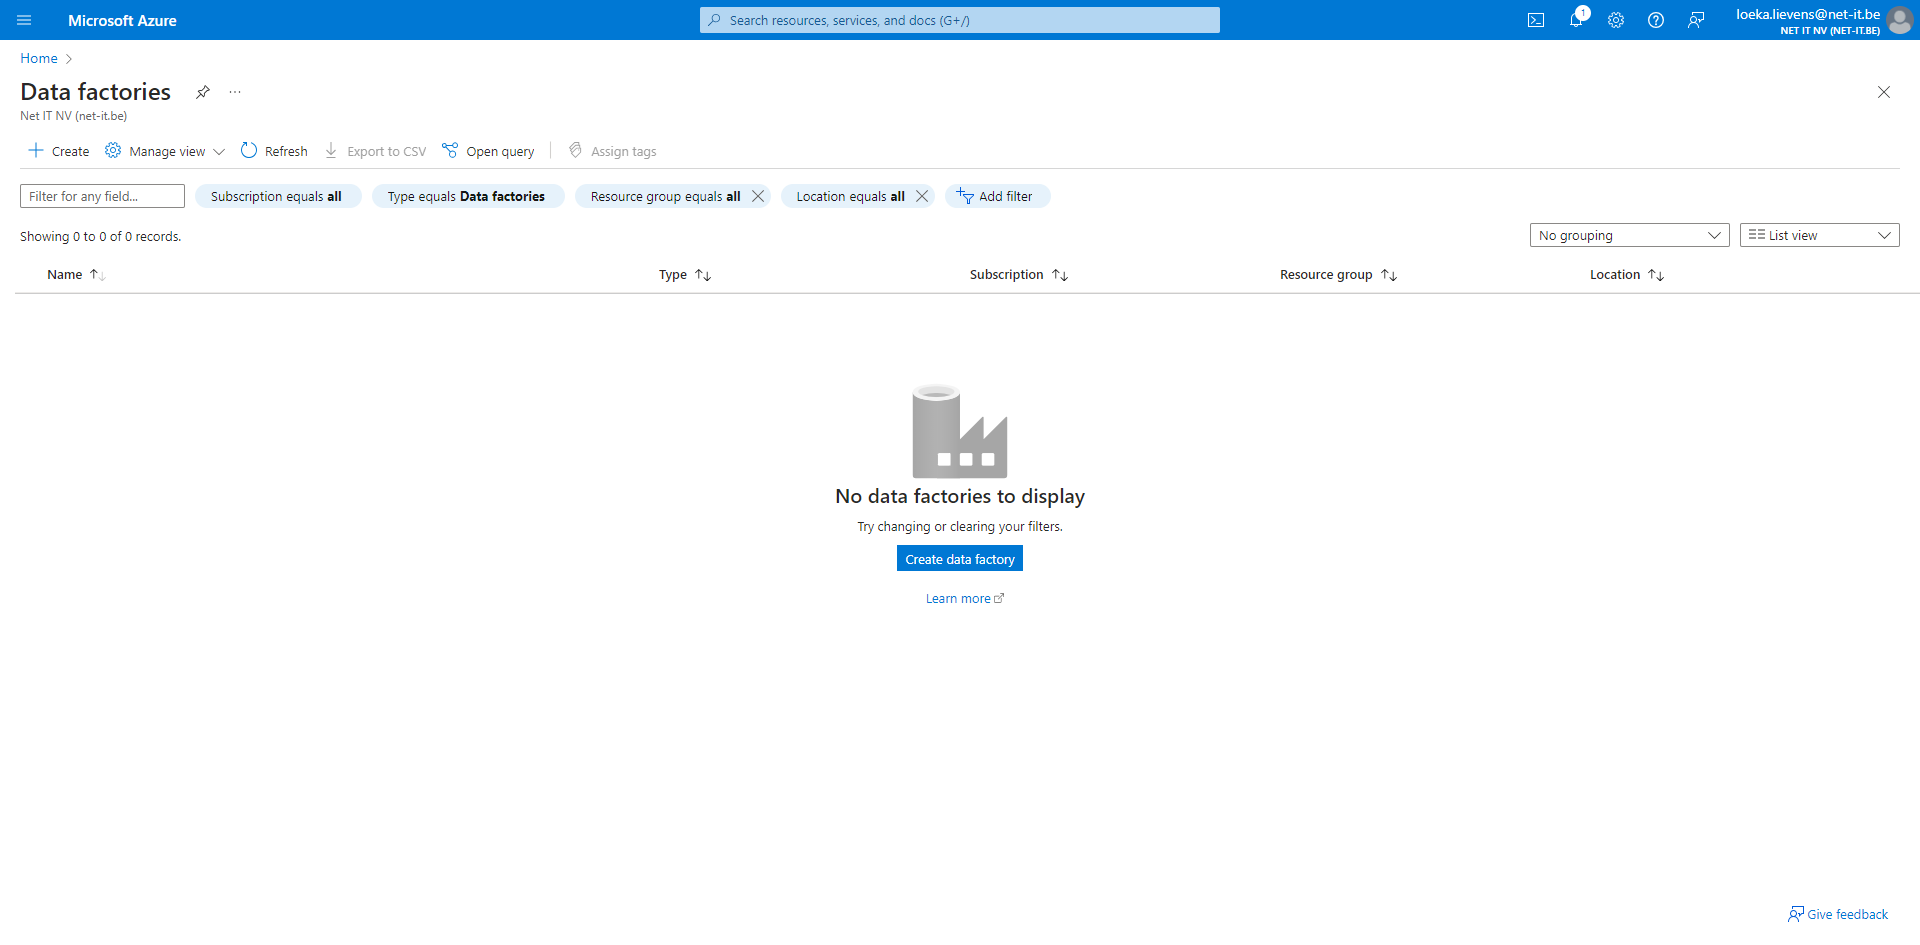
\includegraphics[width=0.6\textwidth]{./graphics/adf/initial.png}
    \footnote{Aanmaken van Azure Data Factory}
\end{center}

Door in Microsoft Azure naar Data Factories te navigeren kunnen we een nieuwe data factory gaan aanmaken.

\begin{center}
    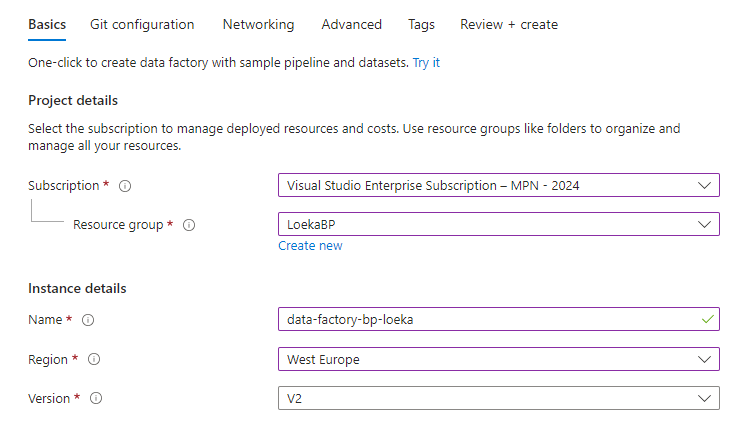
\includegraphics[width=0.6\textwidth]{./graphics/adf/initial_create.png}
    \footnote{Configuratie van Azure Data Factory}
\end{center}

% Resource group en subscription in literatuurstudie
Bij het aanmaken van een data factory moet er een subscription en resource group gekozen worden. Er kan een nieuwe resource group aangemaakt worden of een reeds bestaande gekozen worden. Daarnaast moet er een naam, gewenste regio en versie voor Data Factory gekozen worden. Git configuratie zal later aan bod komen. Data Factory kan nu aangemaakt worden.

\begin{center}
    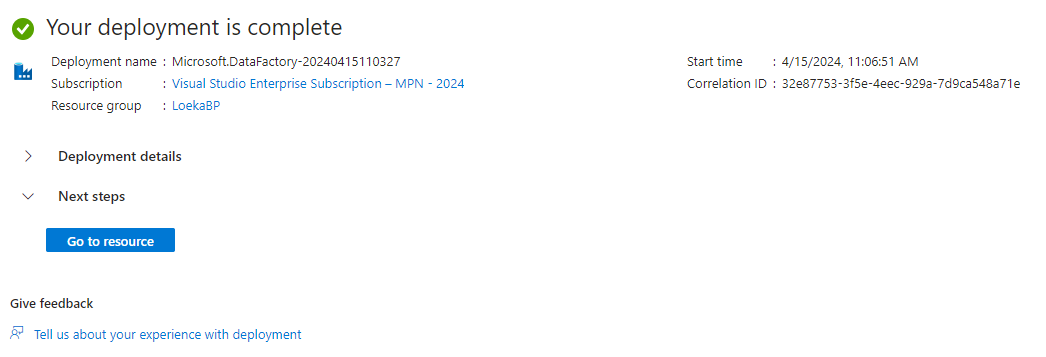
\includegraphics[width=0.6\textwidth]{./graphics/adf/deployment_complete_specific.png}
    \footnote{Deployment complete van Azure Data Factory}
\end{center}

Wanneer de resource is aangemaakt kan Azure Data Factory opgestart worden.

\subsubsection{Collaboration en source control}

Binnen Azure Data Factory kan er op 2 manieren samen gewerkt worden. 

\begin{center}
    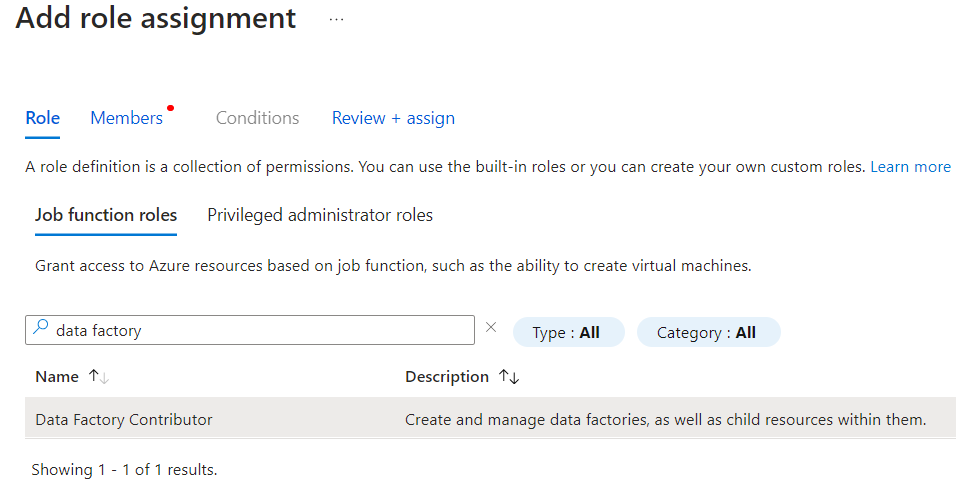
\includegraphics[width=0.6\textwidth]{./graphics/adf/adf_contributor.png}
    \footnote{Toewijzen van Data Factory Contributor Role}
\end{center}

Door de bij de resource group van de data factory de Data Factory Contributor role toe te wijzen kan men toegang geven tot volgende zaken:
\begin{itemize}
    \item Het aanmaken, wijzigen en verwijderen van data factories en child resources
    \item Deployment van Resource Manager templates
    \item Het managen van App Insight alerts voor Data Factory
    \item Het aanmaken van support tickets
\end{itemize}

Daarnaast kan er ook samen gewerkt worden via source control. Azure Data Factory laat het toe om een Git repository te configureren via Azure Repos of GitHub. 

\begin{center}
    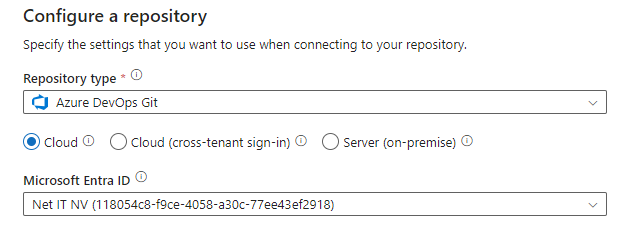
\includegraphics[width=0.6\textwidth]{./graphics/adf/setup_repository_2_specific.png}
    \footnote{Configuratie van Git in Azure Data Factory}
\end{center}

We kiezen voor Azure DevOps doordat er binnen Net IT hiermee gewerkt wordt.

\begin{center}
    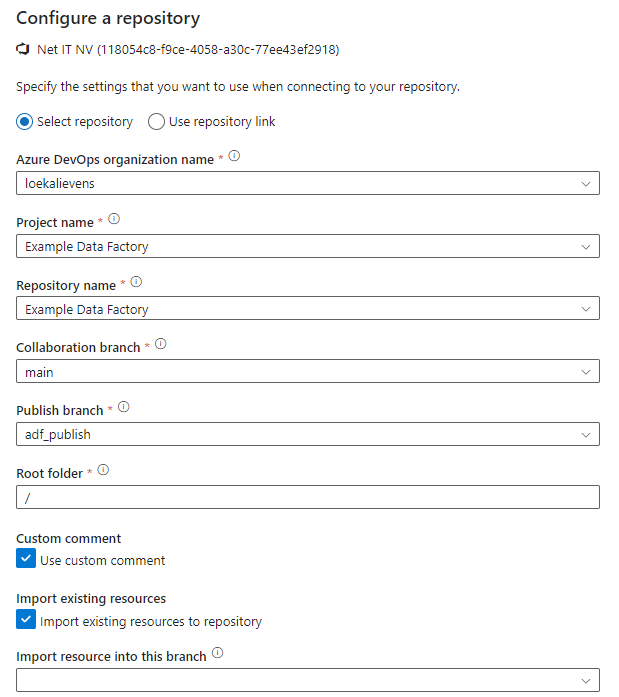
\includegraphics[width=0.6\textwidth]{./graphics/adf/setup_repository_3_specific.png}
    \footnote{Configuratie van Azure DevOps in Azure Data Factory}
\end{center}

De collaboration branch is de enigste branch waarbij de publish knop zichtbaar zal zijn. Door te werken met feature branches en hiermee pull requests te maken op de collaboration branch kan er dus samen gewerkt worden. De publish branch is de branch waar alle ARM templates van de gepubliceerde factory opgeslaan wordt.

\subsubsection{Ophalen van data uit Azure Data Lake}

Het ophalen van data uit Data Lake in Data Flow zal steeds op dezelfde manier gebeuren. 

\begin{center}
    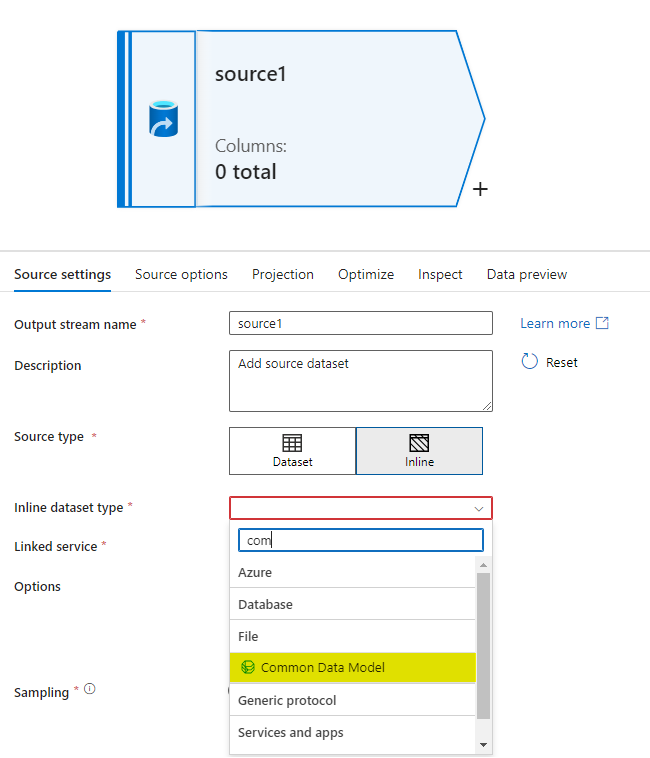
\includegraphics[width=0.6\textwidth]{./graphics/adf/source_table_1_specific.png}
    \footnote{Configuratie van source transformation}
\end{center}

Als source type zal er steeds gekozen worden voor inline. Dit doordat we slechts werken met één enkele dataflow en geen gedeelde datasets nodig hebben. Als inline data set type kiezen we voor Common Data Model.

\begin{center}%
    \centering
    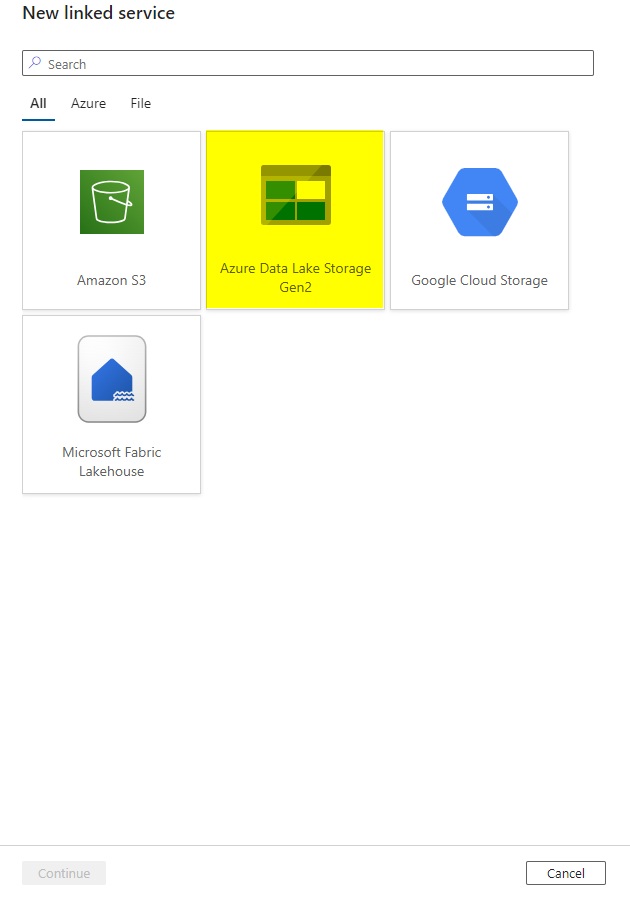
\includegraphics[width=0.4\textwidth]{./graphics/adf/source_table_2_specific}
    \hspace{0.1\textwidth}
    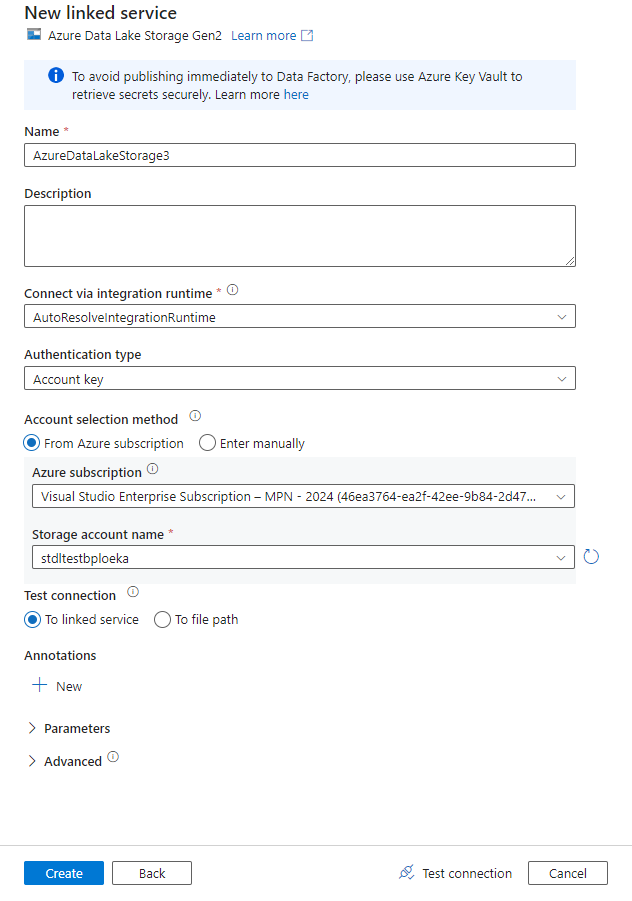
\includegraphics[width=0.4\textwidth]{./graphics/adf/source_table_3_specific}
    \footnote{Configuratie van linked service}
\end{center}

Er zal éénmalig een Linked Service aangemaakt moeten worden. Hierbij kiezen we voor Azure Data Lake Storage Gen2. We kunnen makkelijk gaan koppelen met de juiste data lake door een Azure Subscription en Storage account name aan te duiden. Door op `Test connection` te klikken kunnen we kijken of de connectie met data lake is gelukt. Door op `Create` te klikken hebben we nu een Linked Service die steeds bij elke Source gebruikt kan worden.

\textbf{Let op:} Doordat Git geen secrets opslaat is het aanbevolen om gebruik te maken van Azure Key Vault voor het opslaan van connection strings of passwords.

\begin{center}
    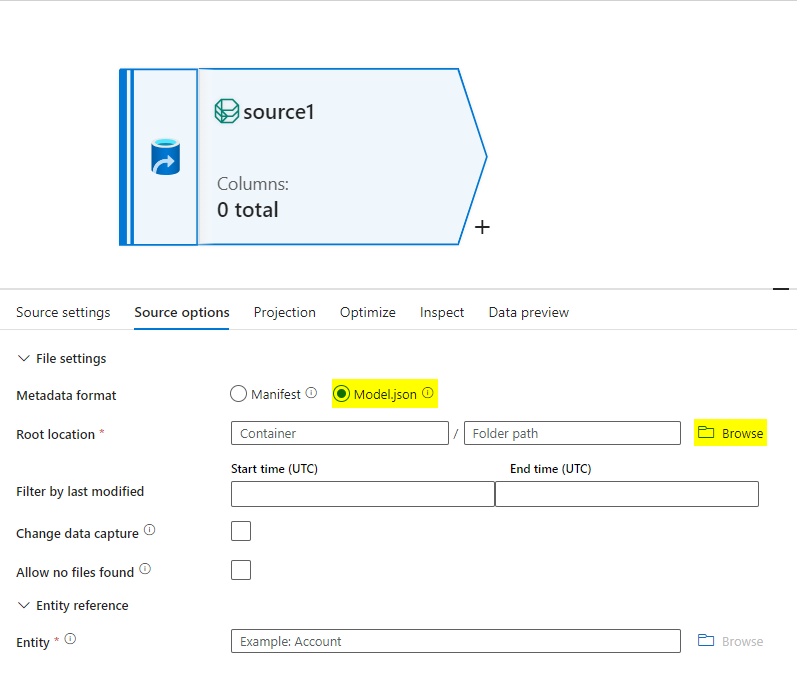
\includegraphics[width=0.6\textwidth]{./graphics/adf/source_table_4_specific.png}
    \footnote{Configuratie van source options}
\end{center}

Door naar `Source options` te gaan kunnen we `Model.json` gaan aanduiden. Door op `Browse` te klikken kunnen we aanduiden waar het Model.json bestand te vinden is in data lake.

\begin{center}
    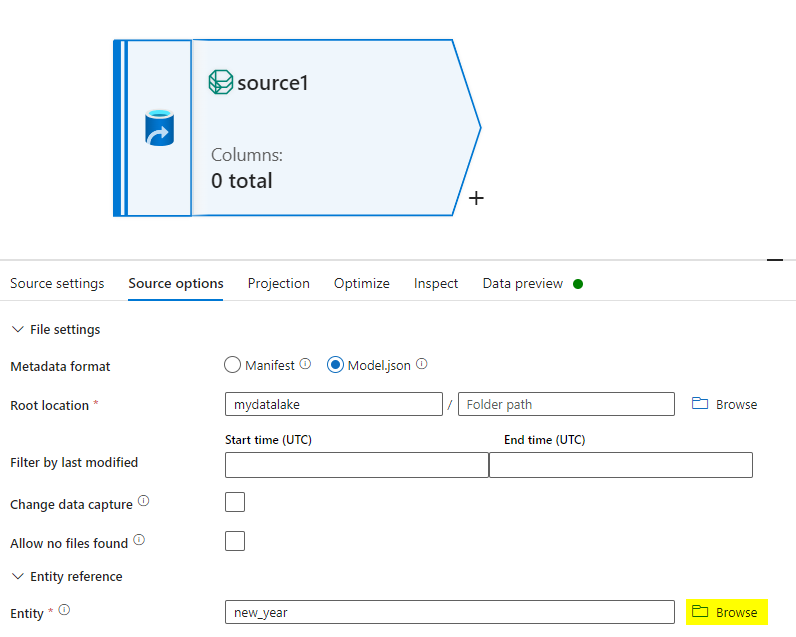
\includegraphics[width=0.6\textwidth]{./graphics/adf/source_table_5_specific.png}
    \footnote{Configuratie van source options}
\end{center}

Naast `Entity` kunnen we nu op `Browse` klikken om de gewenste entity te gaan importeren. Let op: hier voor zal Data flow debug aan moeten staan.

\begin{center}
    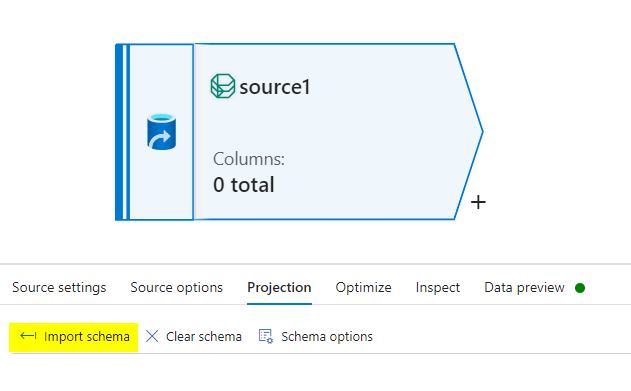
\includegraphics[width=0.6\textwidth]{./graphics/adf/source_table_6_specific.png}
    \footnote{Configuratie van projection}
\end{center}

Door naar `Projection` te gaan kunnen we nu op `Import schema` klikken.

\begin{center}
    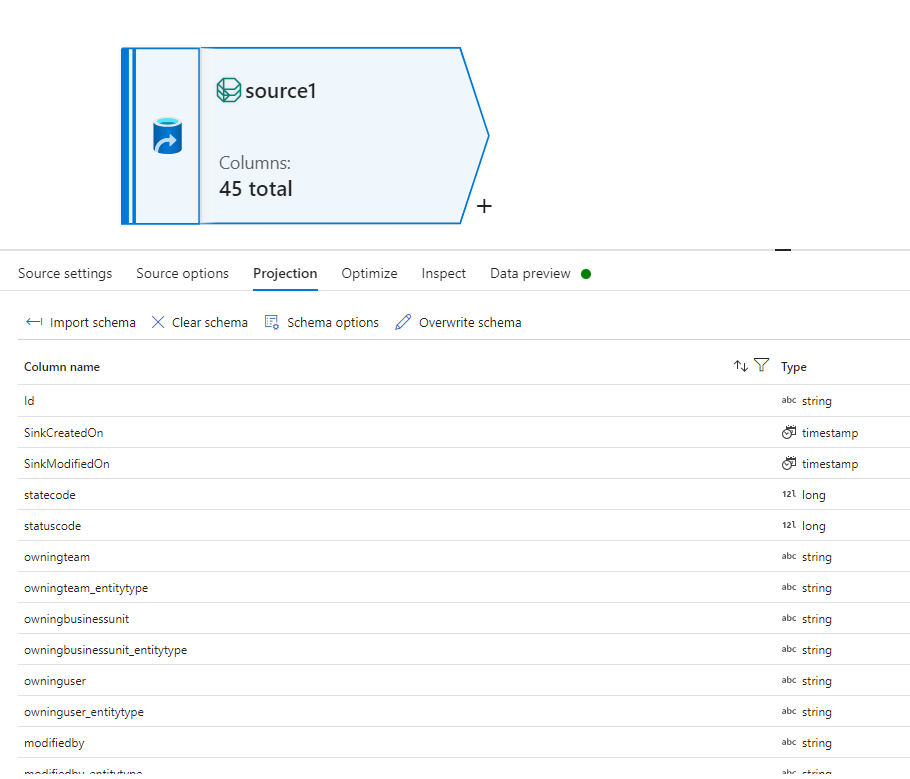
\includegraphics[width=0.6\textwidth]{./graphics/adf/source_table_7_specific.png}
    \footnote{Configuratie van projection}
\end{center}

De foto hierboven toont een voorbeeld van een geïmporteerd schema.

\begin{center}
    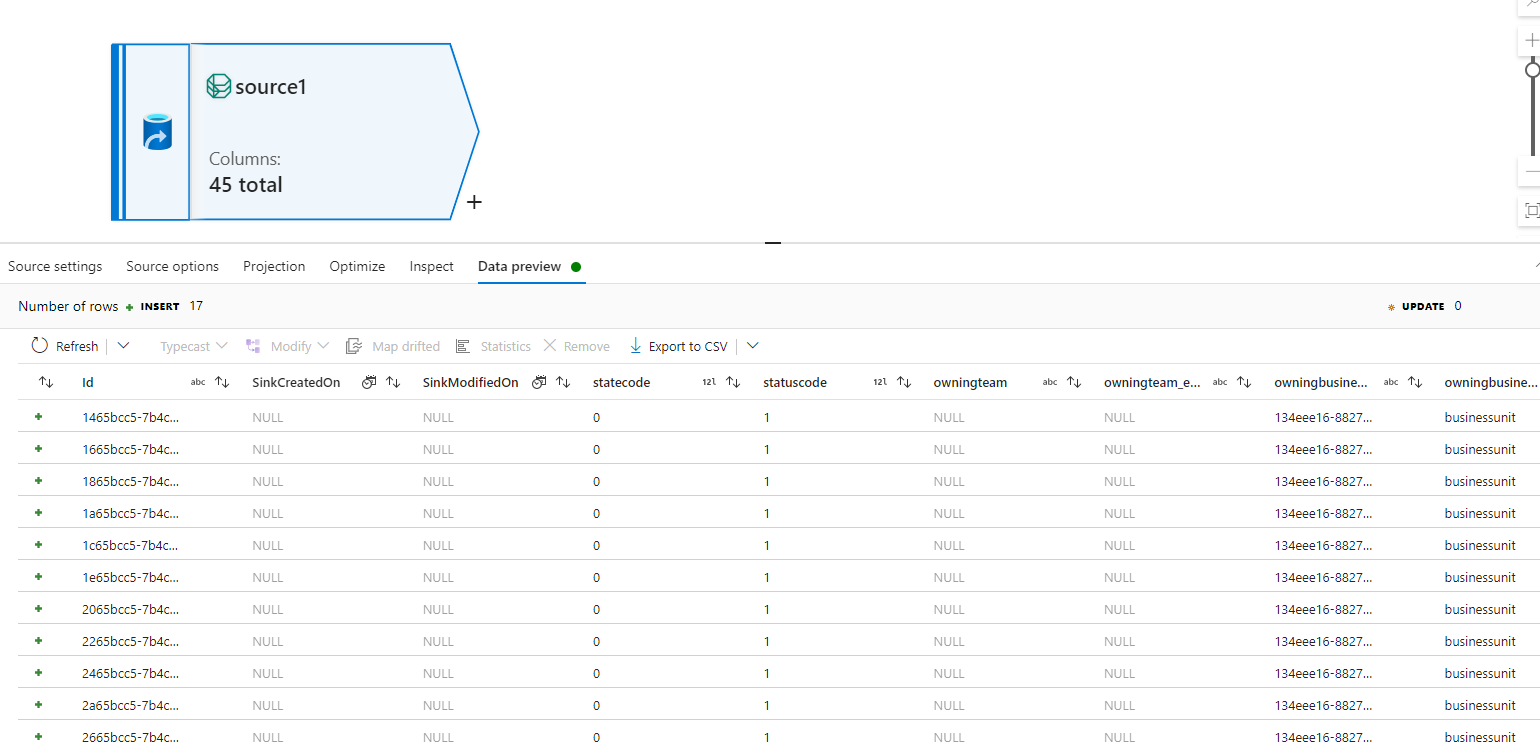
\includegraphics[width=0.6\textwidth]{./graphics/adf/source_table_8_specific.png}
    \footnote{Data preview}
\end{center}

Wanneer we naar `Data preview` gaan kunnen we een preview zien van de data uit de gekozen tabel.

\subsubsection{Belangrijkste transformaties}

Determinatie van welke groepen de premie in hun bestand krijgen

\begin{center}
    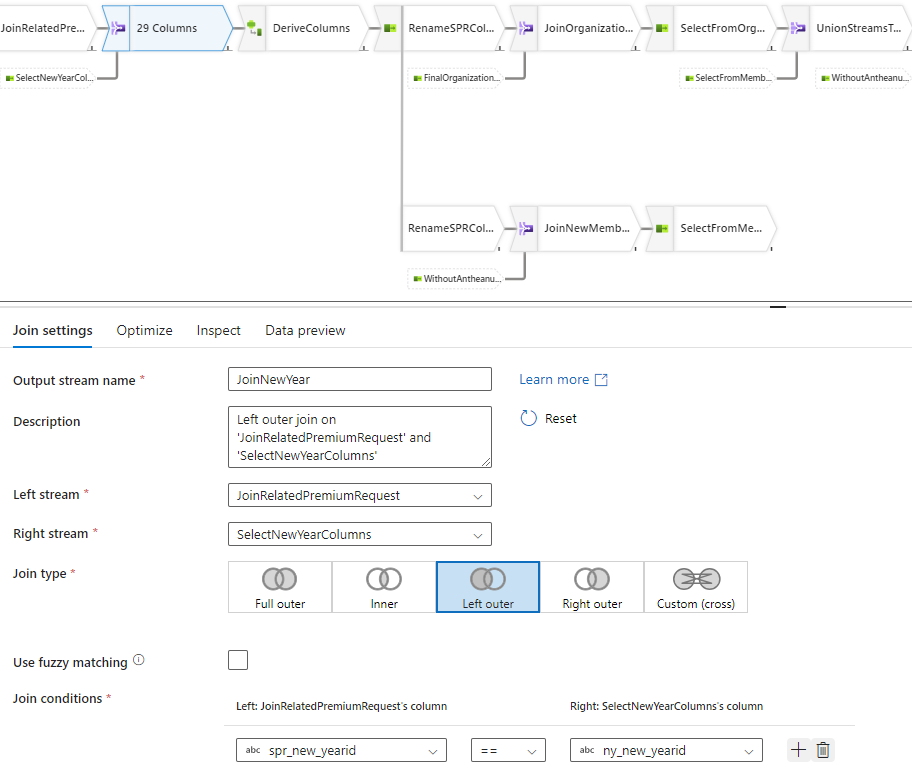
\includegraphics[width=0.6\textwidth]{./graphics/adf/bepalen_groep_1.png}
    \footnote{Join van de tabel `new\_year` op de tabel `new\_syndicalpremiumrequest`}
\end{center}

De tabel `new\_syndicalpremiumrequest` heeft een kolom `spr\_new\_yearid`. Om te gaan bepalen wat het referentiejaar van deze premie is zal dus de tabel `new\_year` op de tabel `new\_syndicalpremiumrequest` gejoind moeten worden aan de hand van dit id.


\begin{center}
    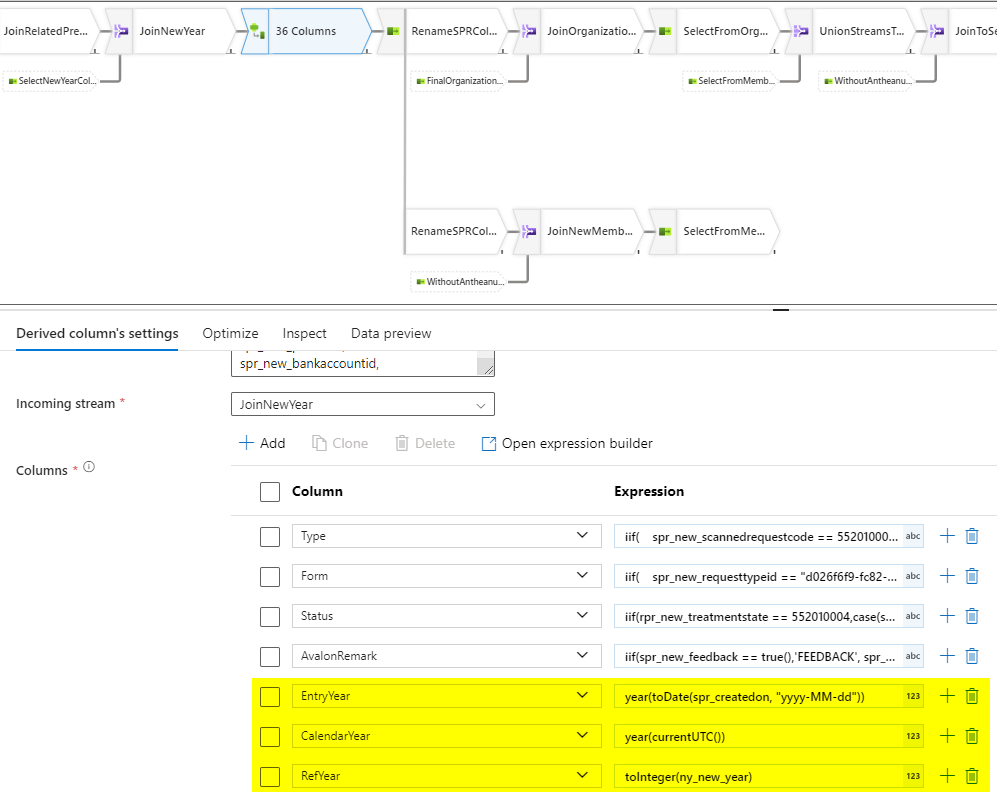
\includegraphics[width=0.6\textwidth]{./graphics/adf/bepalen_groep_2.png}
    \footnote{Derive EntryYear, CalendarYear en RefYear op de tabel `new\_syndicalpremiumrequest`}
\end{center}

Voor het bepalen van de groepen moeten hebben we 3 nieuwe kolommen nodig. Als eerste hebben we het EntryYear nodig, dit is het jaartal van `spr\_createdon`, de datum wanneer de record is aangemaakt. Daarnaast hebben we CalendarYear nodig, dit is het jaartal van de huidige datum. En ten slotte hebben we RefYear nodig, dit is het jaartal van de tabel `new\_year` die net gejoind is geweest.

\begin{center}
    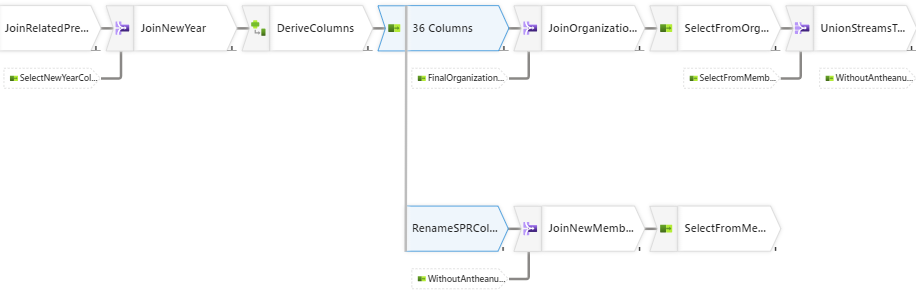
\includegraphics[width=0.6\textwidth]{./graphics/adf/bepalen_groep_3.png}
    \footnote{Hernoemen van `new\_syndicalpremiumrequest` kolommen en splitsing in twee apparte branches}
\end{center}

Vervolgens worden bepaalde kolommen van naam hernoemt. Welke kolommen dit zijn is onbelangrijk voor deze transformatie. Wat wel belangrijk is dat de pipeline zich nu opsplitst in twee apparte branches. Dit doordat er 2 inner joins zullen gebeuren.

\begin{center}
    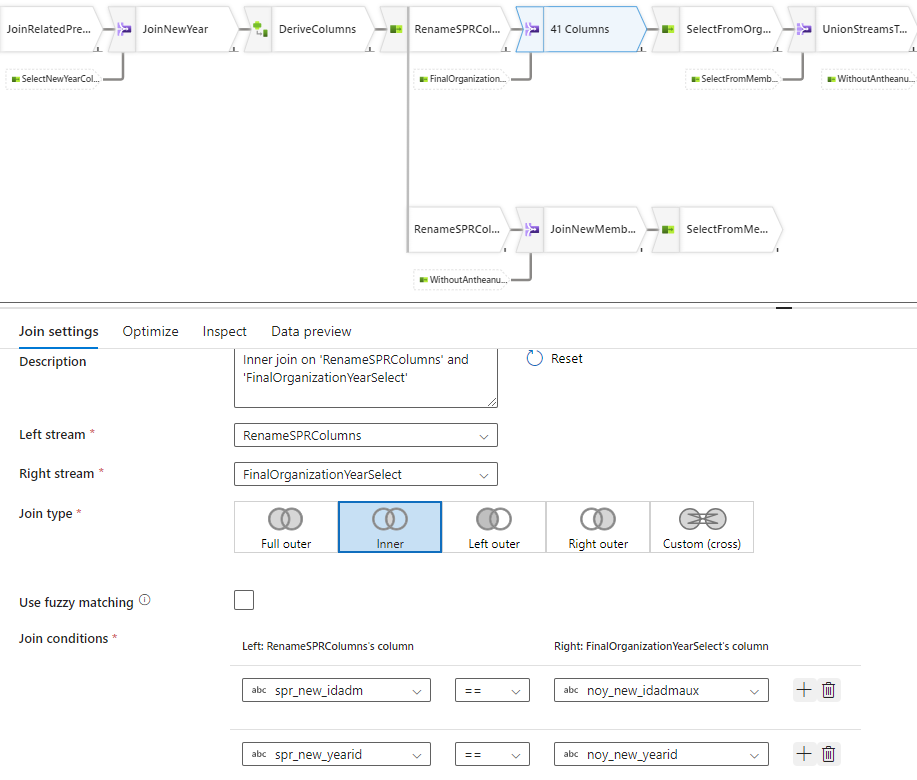
\includegraphics[width=0.6\textwidth]{./graphics/adf/bepalen_groep_4.png}
    \footnote{Inner join van `new\_organizationyear` op de tabel `new\_syndicalpremiumrequest`}
\end{center}

Er gebeurt nu een inner join van de tabel `new\_organizationyear` op de tabel `new\_syndicalpremiumrequest`. Hierbij wordt er aan de hand van IDADM en het id van het referentiejaar gejoind.

\begin{center}
    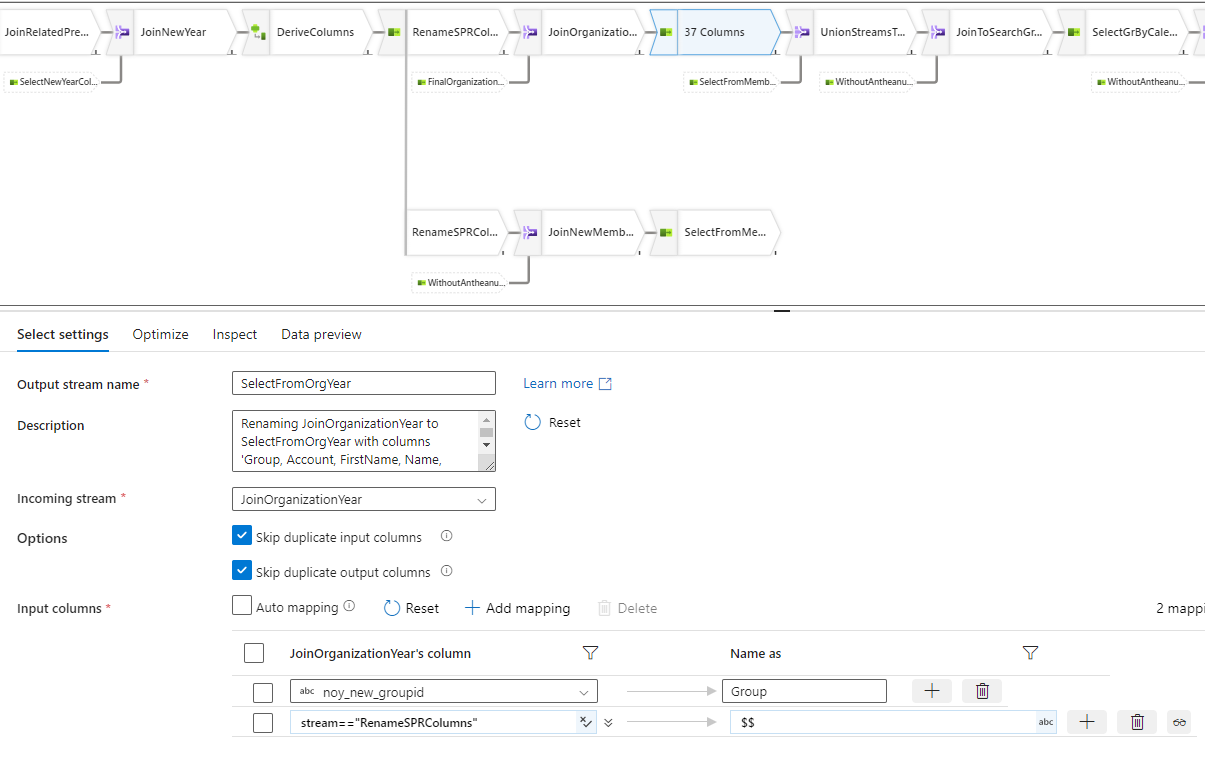
\includegraphics[width=0.6\textwidth]{./graphics/adf/bepalen_groep_5.png}
    \footnote{Selecteren en hernoemen van kolommen op de tabel `new\_syndicalpremiumrequest`}
\end{center}

Vervolgens worden alle kolommen die er voor de join waren geselecteerd. Daarnaast wordt er één kolom `noy\_new\_groupid` geselecteerd en hernoemd naar `Group`.

\begin{center}
    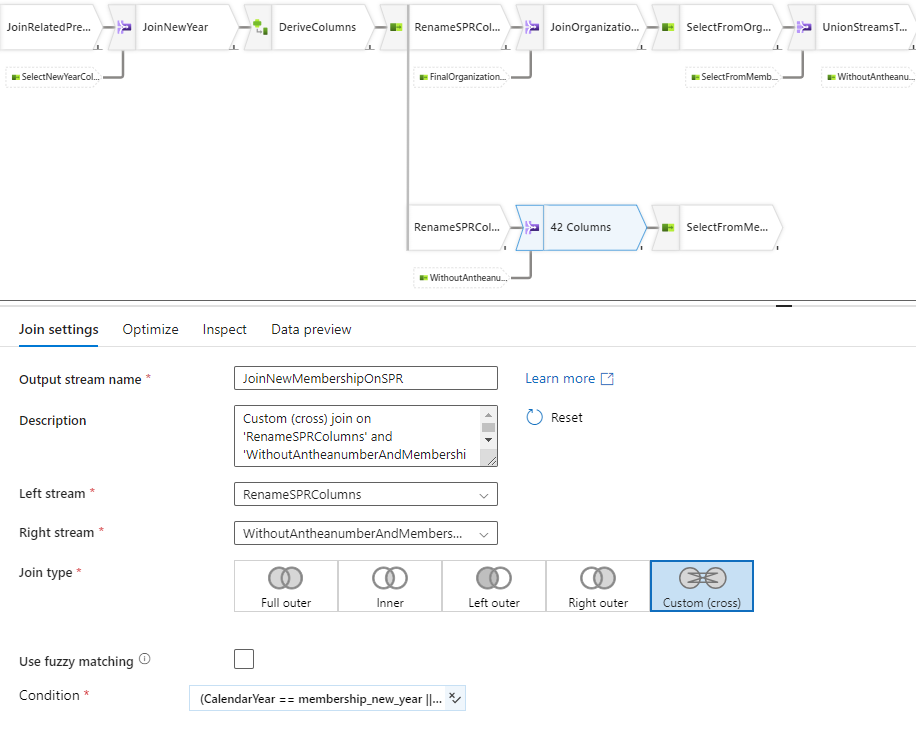
\includegraphics[width=0.6\textwidth]{./graphics/adf/bepalen_groep_6.png}
    \footnote{Custom (cross) join van `new\_membership` op de tabel `new\_syndicalpremiumrequest`}
\end{center}

Bij de tweede branch wordt de tabel `new\_membership` gejoind op de tabel `new\_syndicalpremiumrequest`. Er wordt gebruik gemaakt van een custom (cross) join doordat er OR condities worden gebruikt. 

\begin{center}
    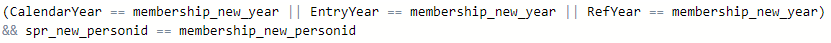
\includegraphics[width=0.6\textwidth]{./graphics/adf/bepalen_groep_7.png}
    \footnote{Conditie van de custom (cross) join van `new\_membership` op de tabel `new\_syndicalpremiumrequest`}
\end{center}

In de conditie van de custom (cross) join wordt er vergeleken of CalendarYear, EntryYear of RefYear overeenkomt met het jaartal van de membership. Daarnaast wordt er ook gekeken of personid overeen komt.

\begin{center}
    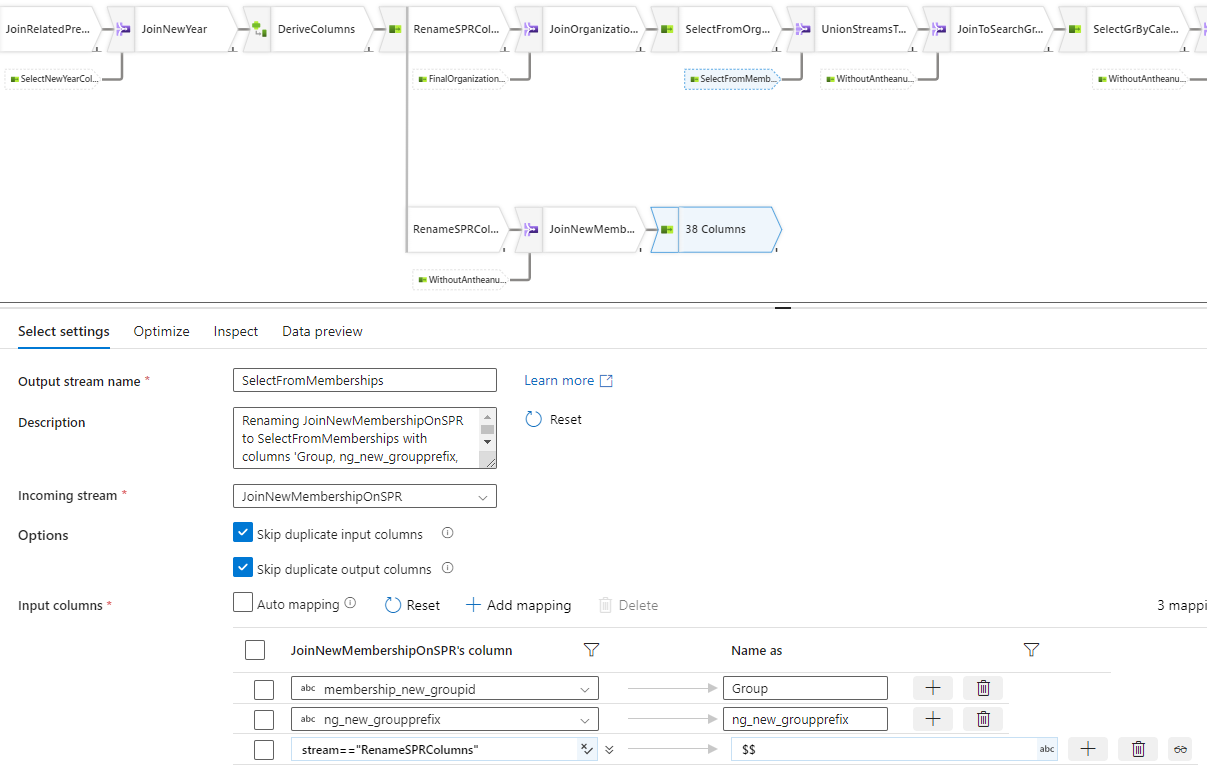
\includegraphics[width=0.6\textwidth]{./graphics/adf/bepalen_groep_8.png}
    \footnote{Selecteren en hernoemen van kolommen op de tabel `new\_syndicalpremiumrequest`}
\end{center}

Ook na deze join worden alle kolommen die er voor de join waren geselecteerd. Daarnaast wordt er 1 kolom `membership\_new\_groupid` geselecteerd en hernoemd naar `Group`. Ten slotte wordt de kolom `ng\_new\_groupprefix` geselecteerd maar dit heeft te maken met een andere transformatie.

\begin{center}
    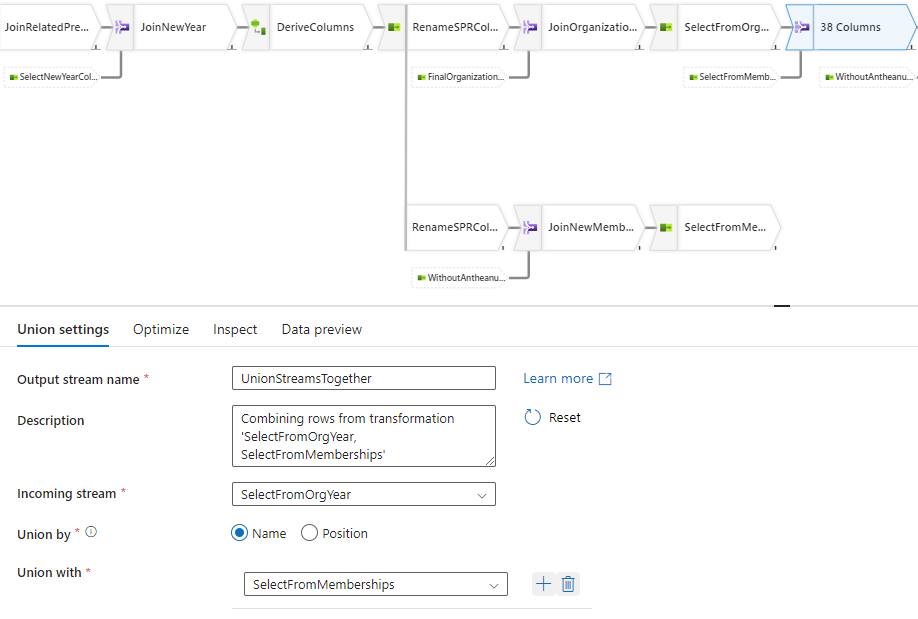
\includegraphics[width=0.6\textwidth]{./graphics/adf/bepalen_groep_9.png}
    \footnote{Union van twee branches}
\end{center}

Beide branches hebben nu dezelfde kolommen met een extra kolom `Group`. Daarnaast heeft de onderste branch nog één extra kolom `ng\_new\_groupprefix`. De beide branches worden nu samen gevoegd met behulp van een union. De bovenste branch die de kolom `ng\_new\_groupprefix` niet heeft zal voor deze kolom de waarde `NULL` krijgen in de records komende van deze branch. 

% TODO group by uitleggen

\subsection{Azure Databricks}

\subsubsection{Opzet van resources}

\begin{center}
    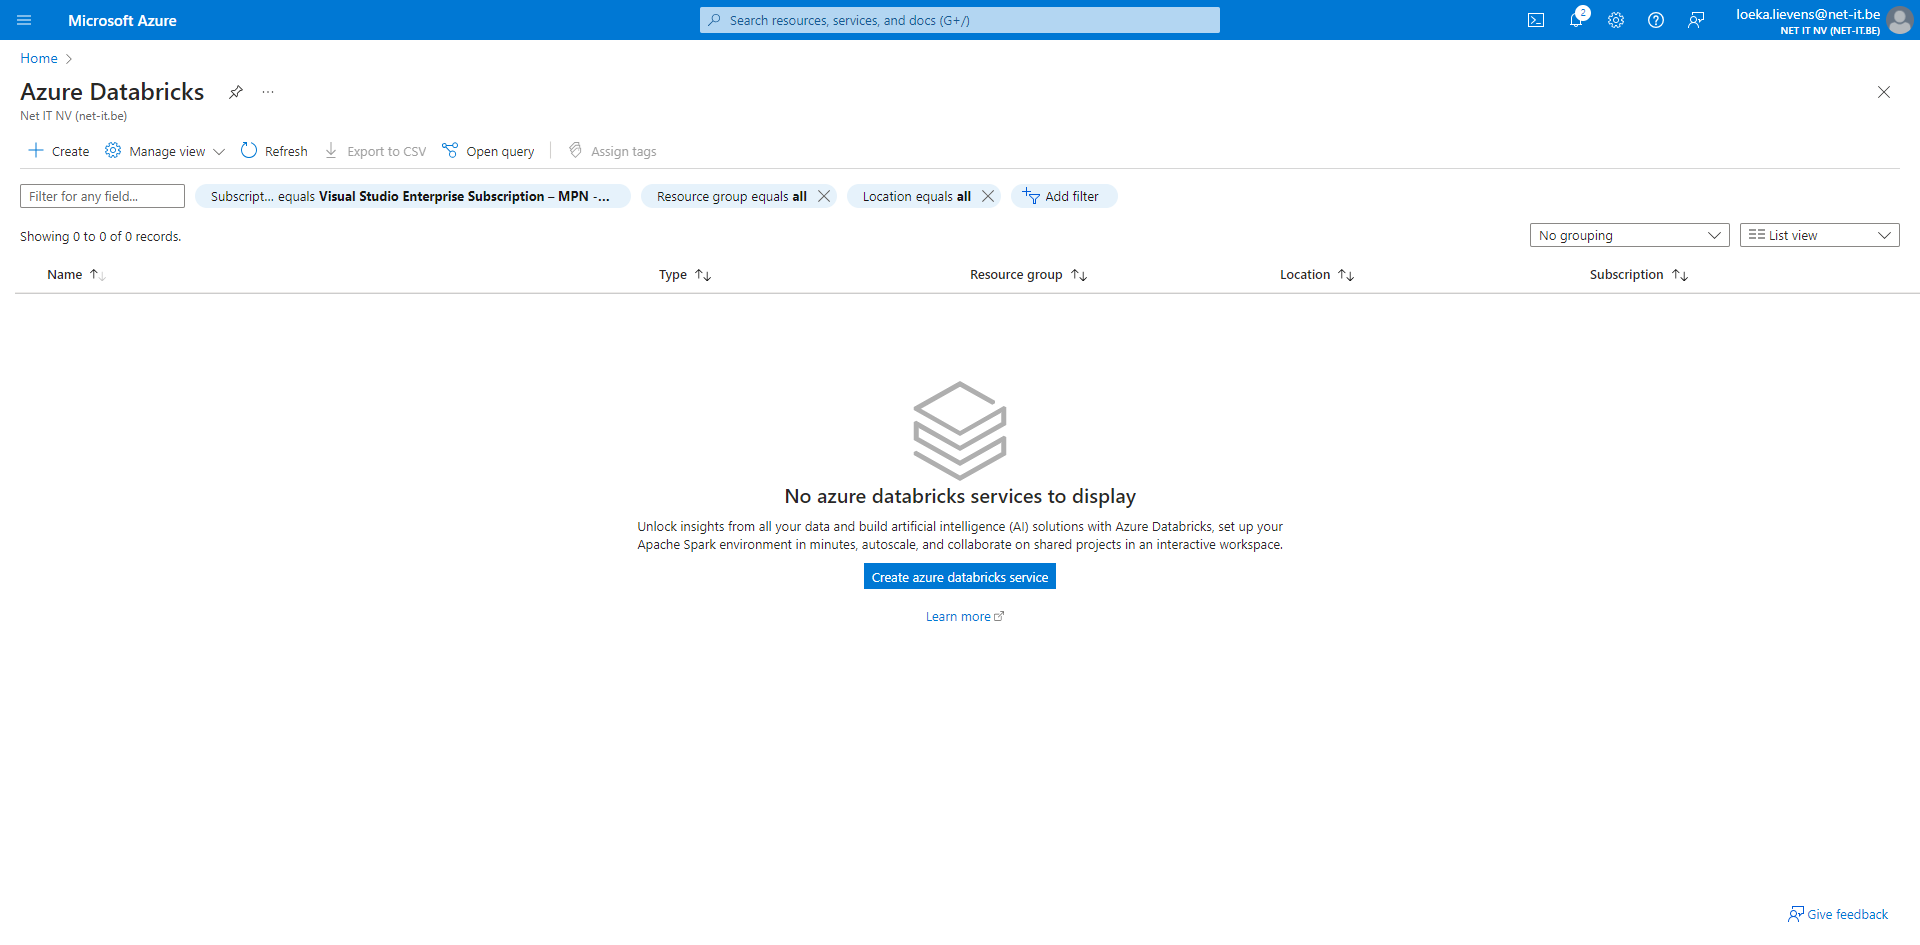
\includegraphics[width=0.9\textwidth]{./graphics/databricks/initial_1.png}
    \footnote{Aanmaken van Azure Databricks}
\end{center}

Door in Microsoft Azure naar Databricks te navigeren kunnen we een nieuwe Azure Databricks workspace gaan aanmaken.

\begin{center}
    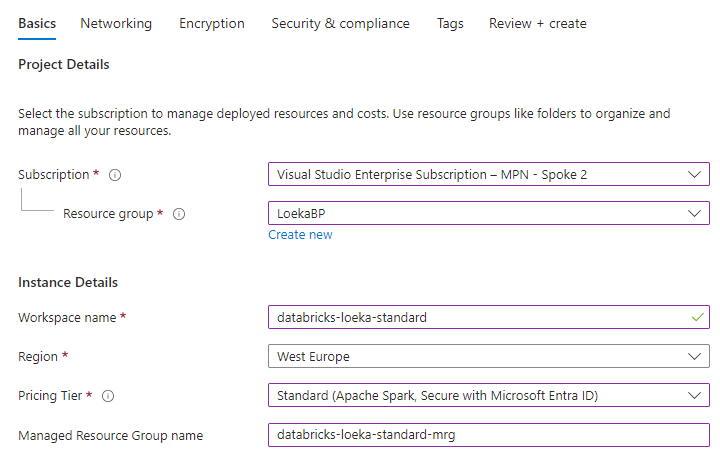
\includegraphics[width=0.6\textwidth]{./graphics/databricks/initial_2.png}
    \footnote{Configuratie van Azure Databricks}
\end{center}

Bij het aanmaken van databricks moet er een subscription en resource group gekozen worden. Er kan een nieuwe resource group aangemaakt worden of een reeds bestaande gekozen worden. Daarnaast moet er een naam, gewenste regio en pricing tier gekozen worden. Als pricing tier kiezen we hier voor Standard doordat we geen gebruik gaan maken van Premium features. Ten slotte kan er ook een Managed Resource Group name gekozen worden. Deze resource group houdt alle resource bij die databricks nodig heeft, zoals bijvoorbeeld virtual machines, storage accounts en virtual networks.

\begin{center}
    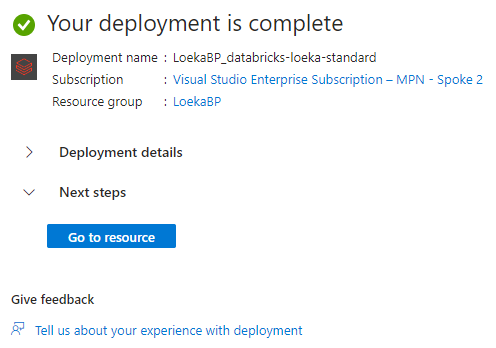
\includegraphics[width=0.6\textwidth]{./graphics/databricks/initial_3.png}
    \footnote{Deployment complete van Azure Databricks}
\end{center}

Wanneer de resource is aangemaakt kan Azure Databricks opgestart worden.

\begin{center}
    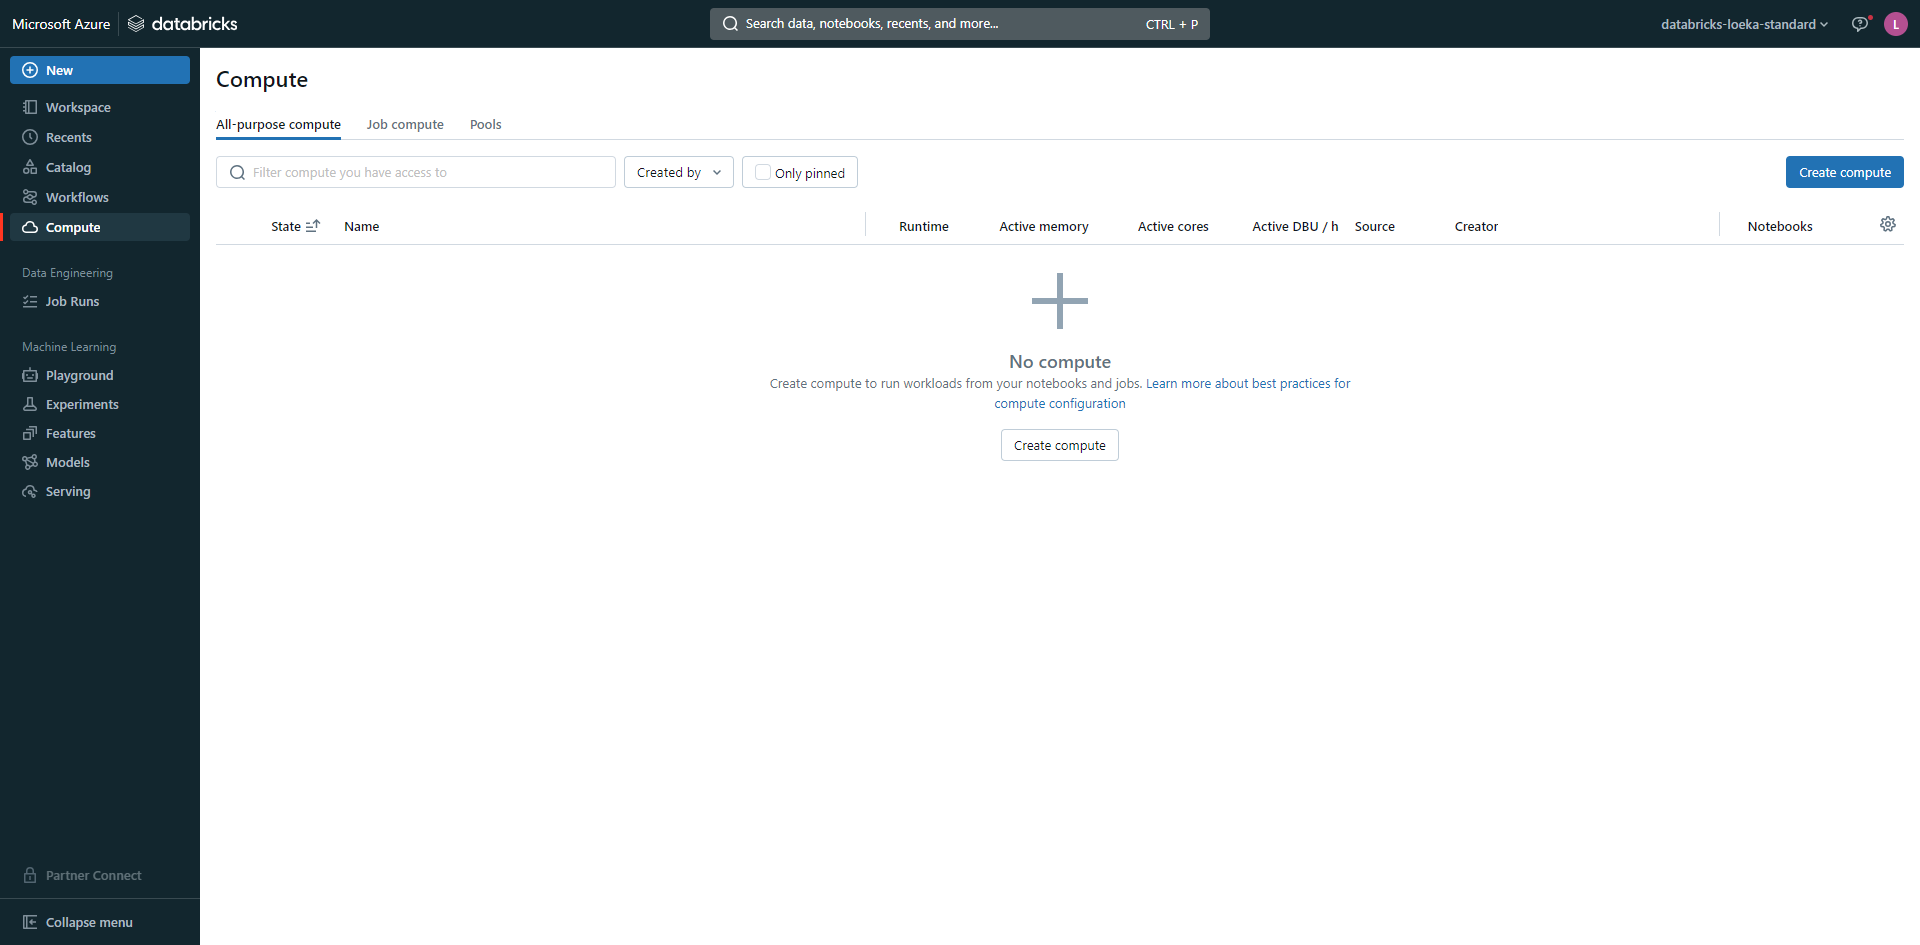
\includegraphics[width=0.9\textwidth]{./graphics/databricks/initial_4.png}
    \footnote{Aanmaken van compute resource}
\end{center}

Voor we notebooks en jobs gaan kunnen uitvoeren zullen we eerst een compute resource moeten gaan aanmaken.

\begin{center}
    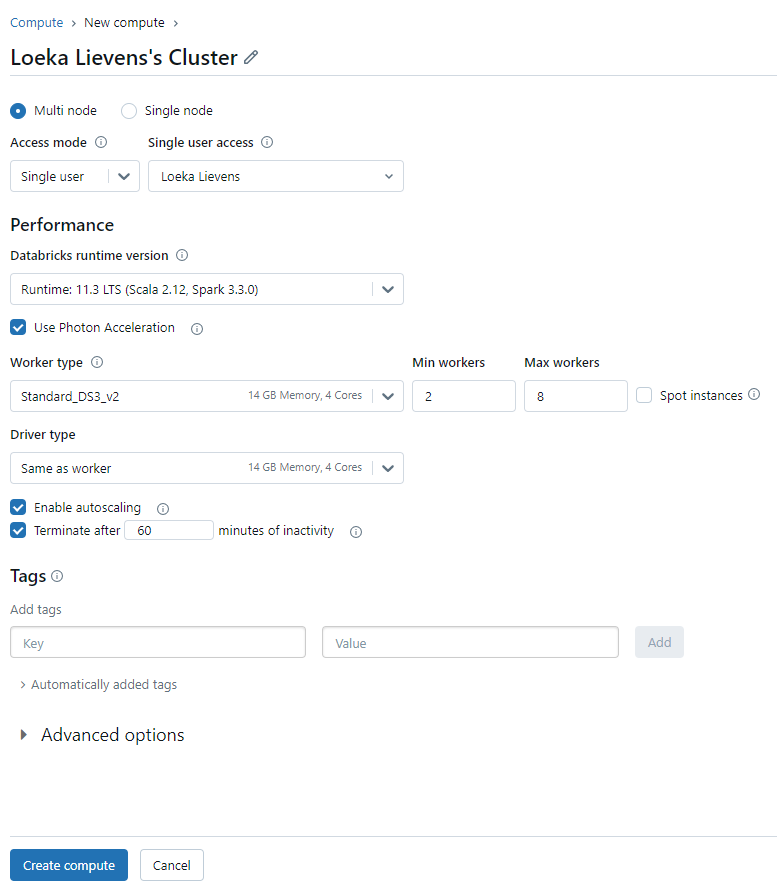
\includegraphics[width=0.6\textwidth]{./graphics/databricks/initial_5.png}
    \footnote{Configuratie van compute resource}
\end{center}

De databricks runtime version moet op 11.3 LTS gezet worden zodat we Apache Spark 3.3.0 kunnen gebruiken. Dit omdat we gebruik gaan maken van `spark-cdm-connector`. Ook hebben we ingesteld dat de cluster zichzelf zal uitschakelen na 60 minuten om onnodige kosten te voorkomen.

\begin{center}
    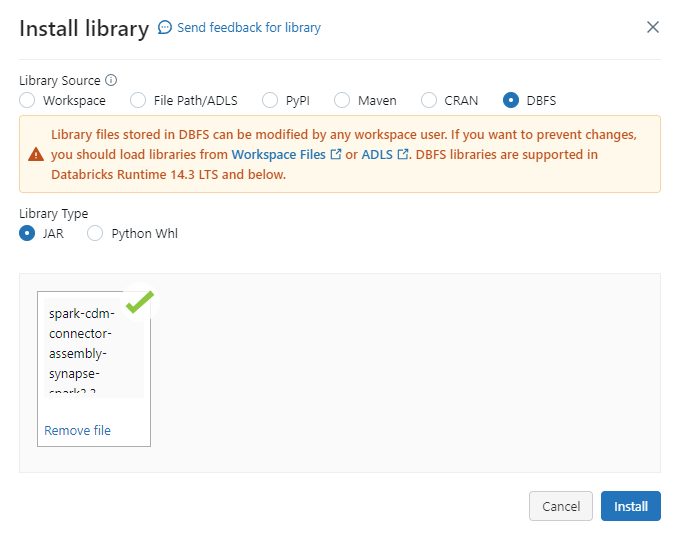
\includegraphics[width=0.9\textwidth]{./graphics/databricks/initial_6.png}
    \footnote{Installatie van `spark-cdm-connector`}
\end{center}

Ten slotte moet de \href{https://github.com/Azure/spark-cdm-connector/releases/tag/spark3.3-1.19.5}{jar file} van `spark-cdm-connector` geïnstalleerd worden in het aangemaakte compute resource om gebruik te kunnen maken van het Common Data Model in onze pipeline.

\subsection{Collaboration en source control}

Databricks folders is een visuele Git client binnen Azure Databricks om gebruik te kunnen maken van source control.

\begin{center}
    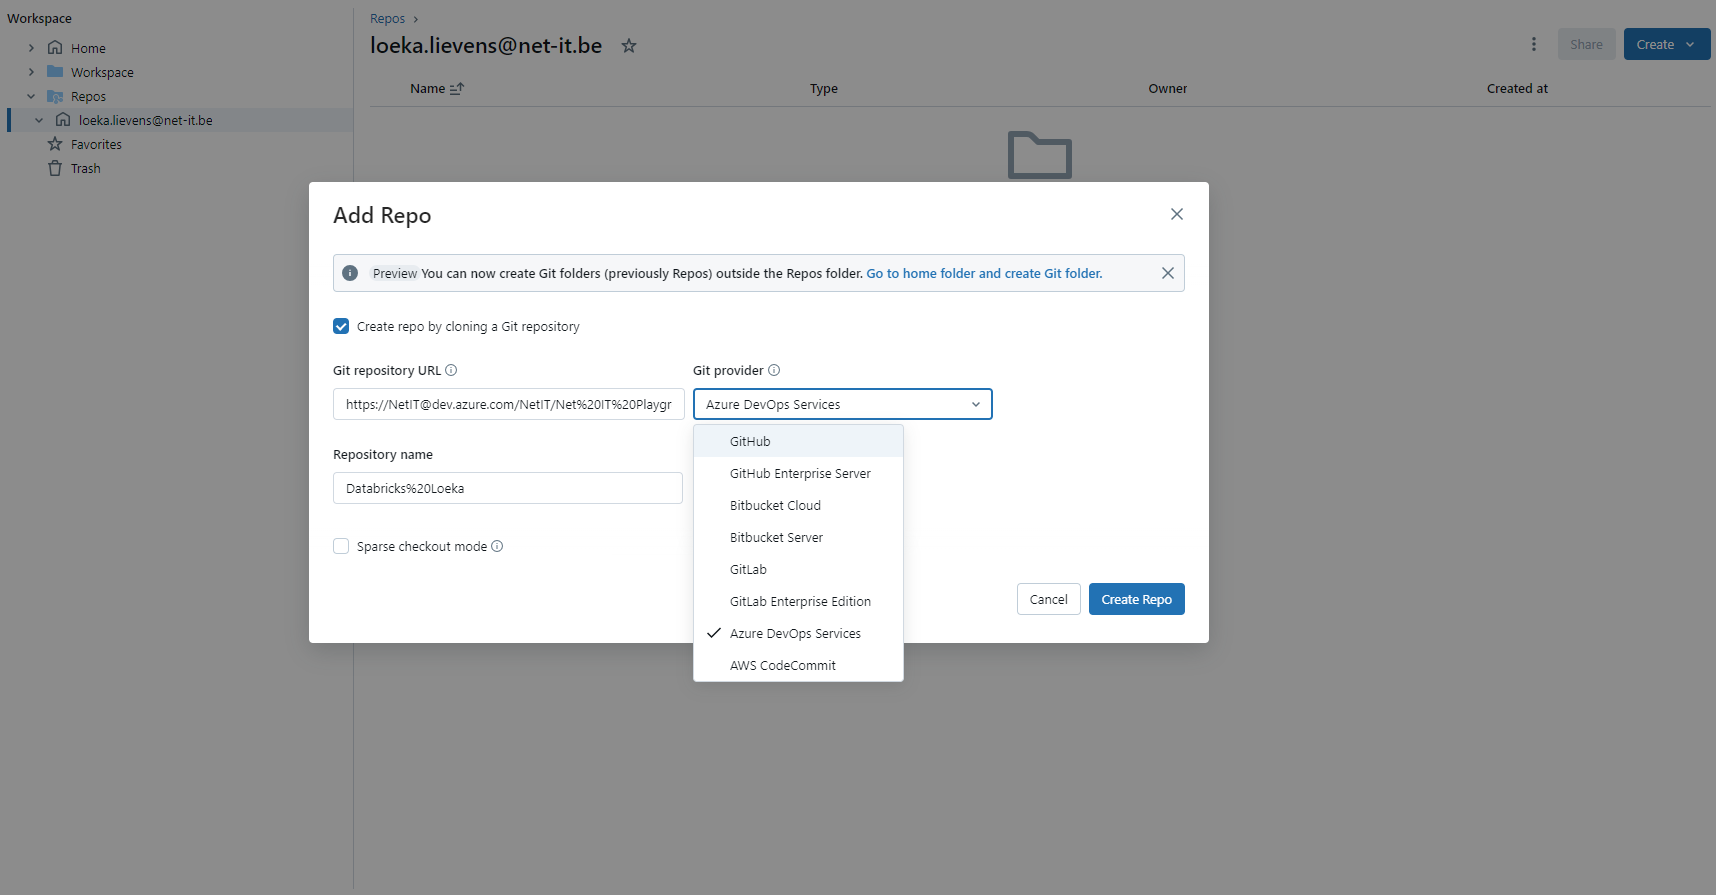
\includegraphics[width=0.9\textwidth]{./graphics/databricks/git_1.png}
    \footnote{Clone Git repository in Databricks folders}
\end{center}

Het geeft de optie om verschillende Git providers te gaan gebruiken. Doordat er binnen Net IT gewerkt wordt met Azure DevOps Services zal hier voor gekozen worden.

\begin{center}
    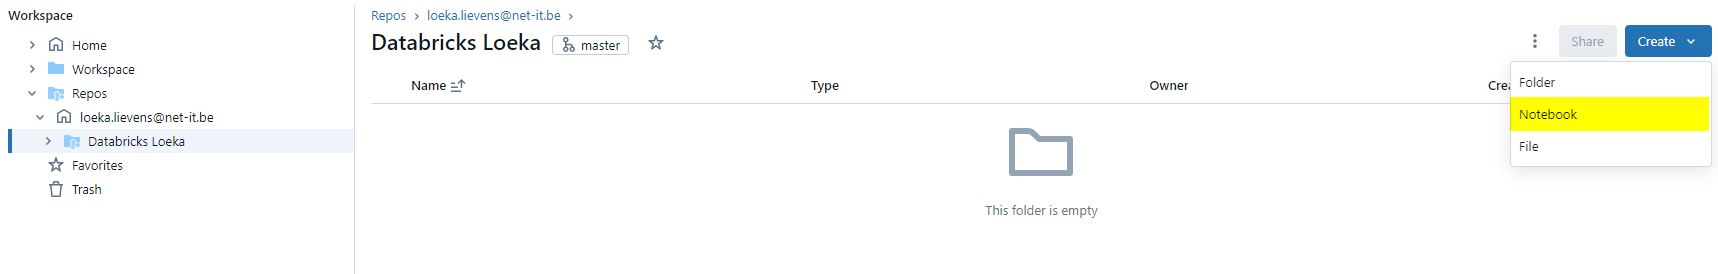
\includegraphics[width=0.9\textwidth]{./graphics/databricks/git_2.png}
    \footnote{Aanmaken van een notebook in databricks}
\end{center}

Ter illustratie zal er een voorbeeld notebook aangemaakt worden.

\begin{center}
    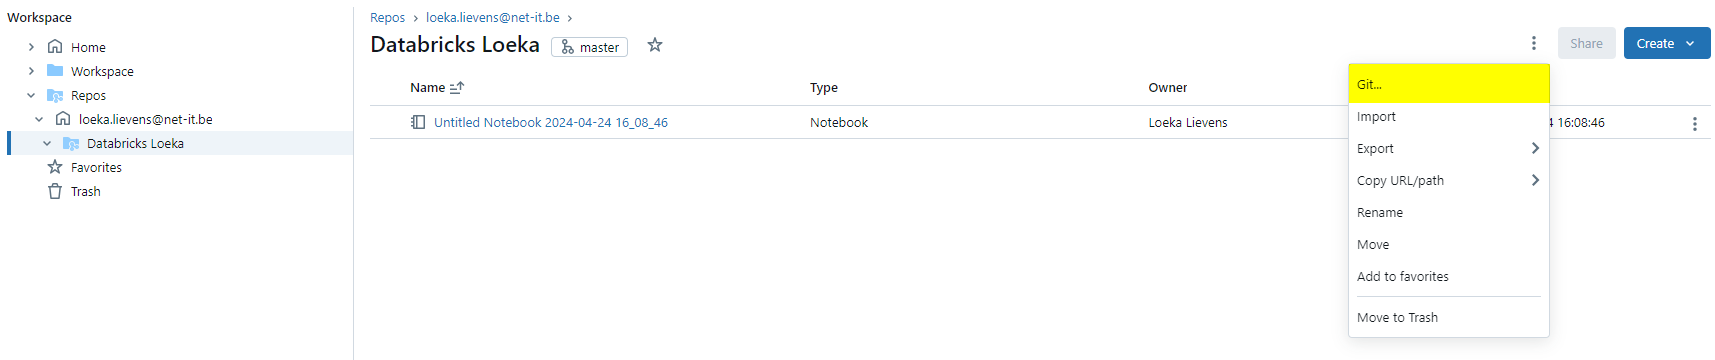
\includegraphics[width=0.9\textwidth]{./graphics/databricks/git_3.png}
    \footnote{Commit en push in Databricks}
\end{center}

\begin{center}
    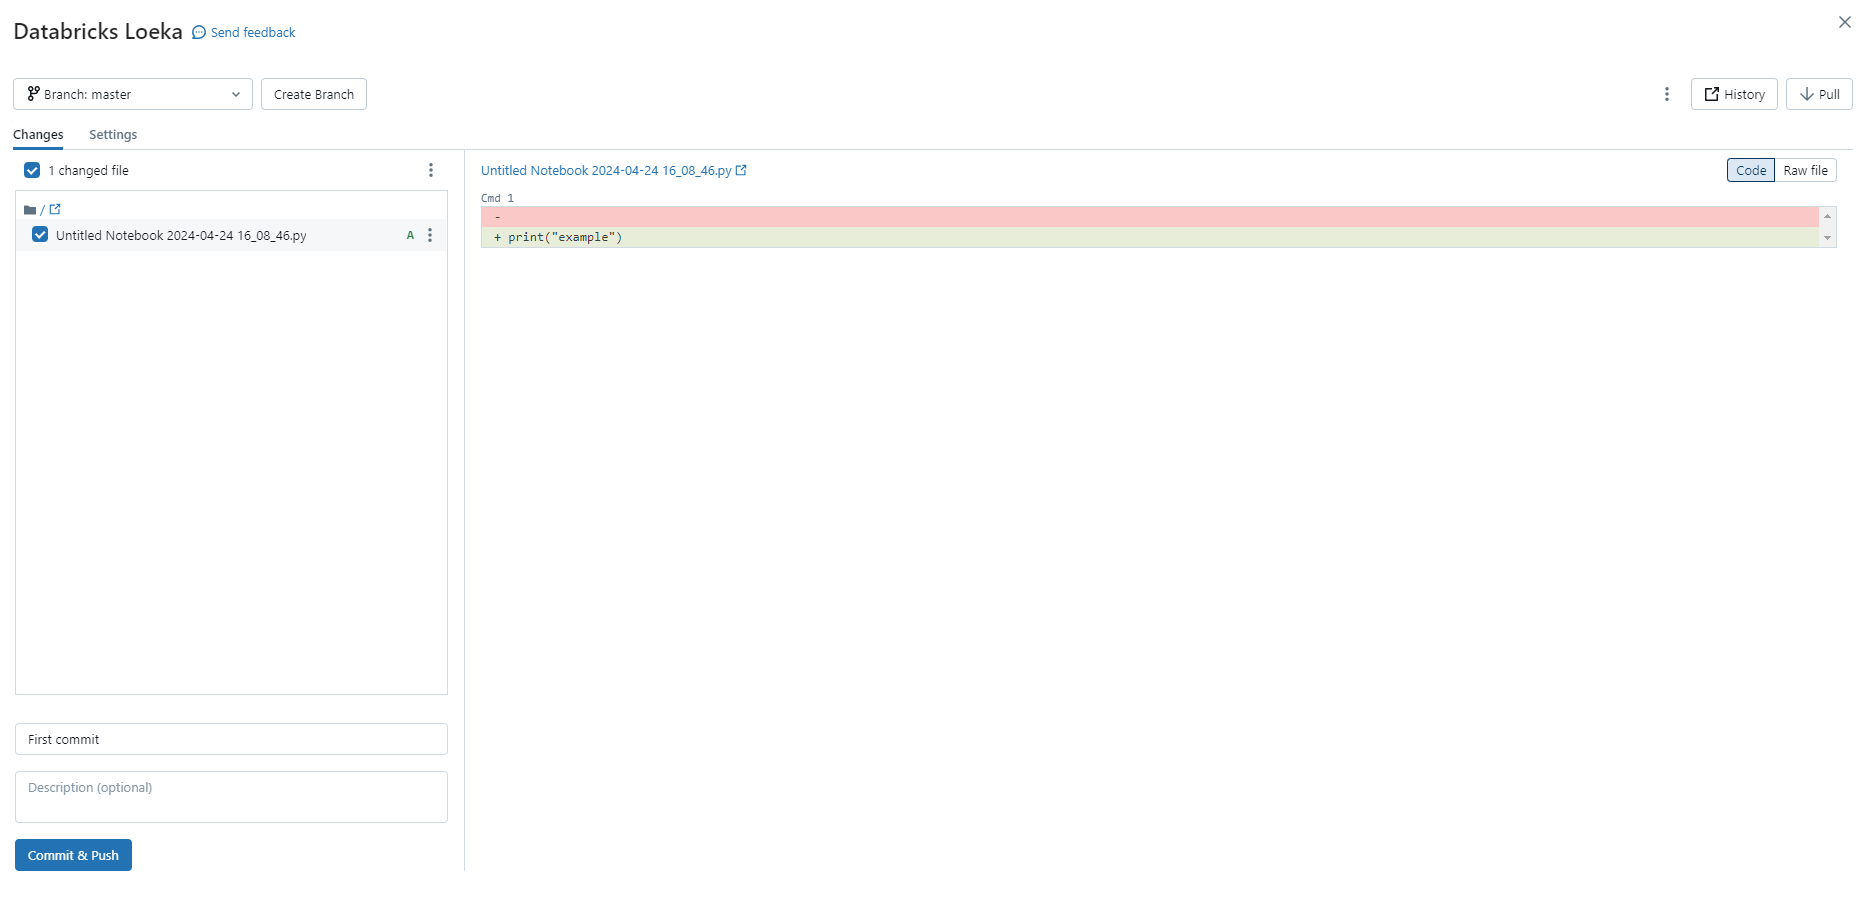
\includegraphics[width=0.9\textwidth]{./graphics/databricks/git_4.png}
    \footnote{Commit en push in Databricks}
\end{center}

Deze notebook kan dan gecommit worden naar Git.

% Einde nieuw

%\begin{center}
%    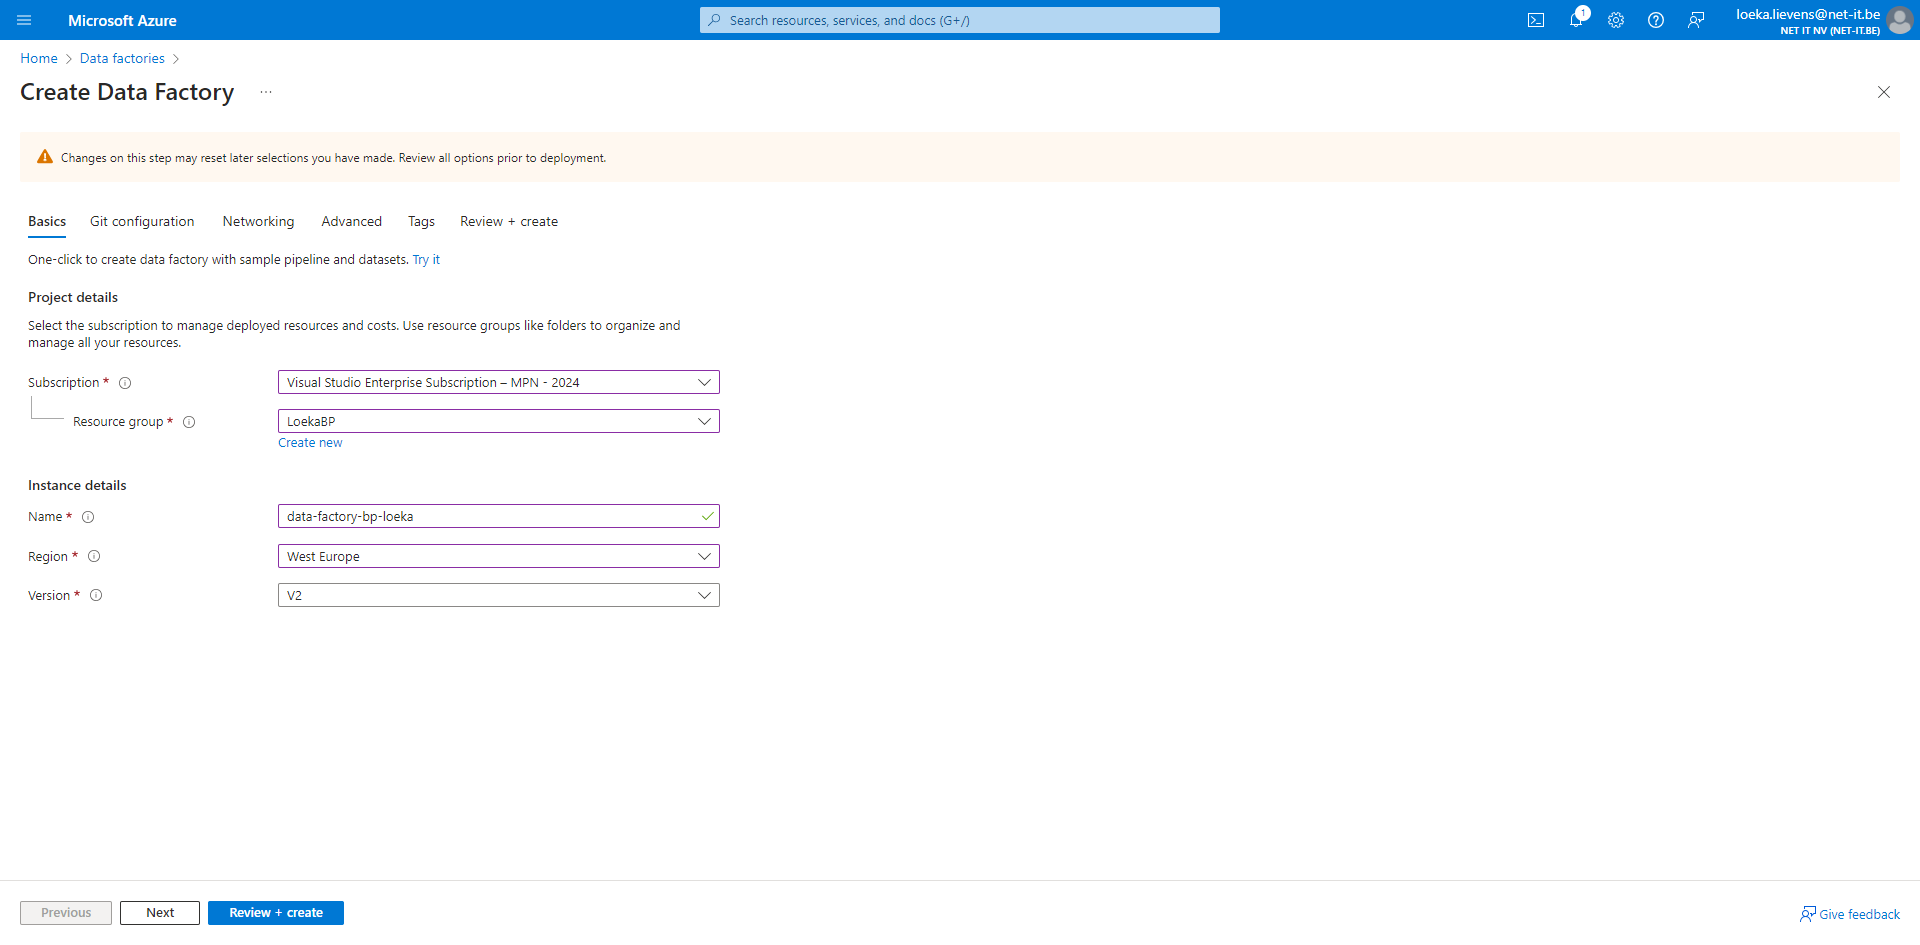
\includegraphics[width=1\textwidth]{./graphics/adf/initial_1.png}
%\end{center}
%
%Selecteer een gewenste subsscription en resource group. Er kan gekozen worden voor een resource group die er al bestaat of om een nieuwe aan te maken. Hier na kan er een naam en gewenste regio gekozen worden. De version laten we staan op V2.
%
%\begin{center}
%    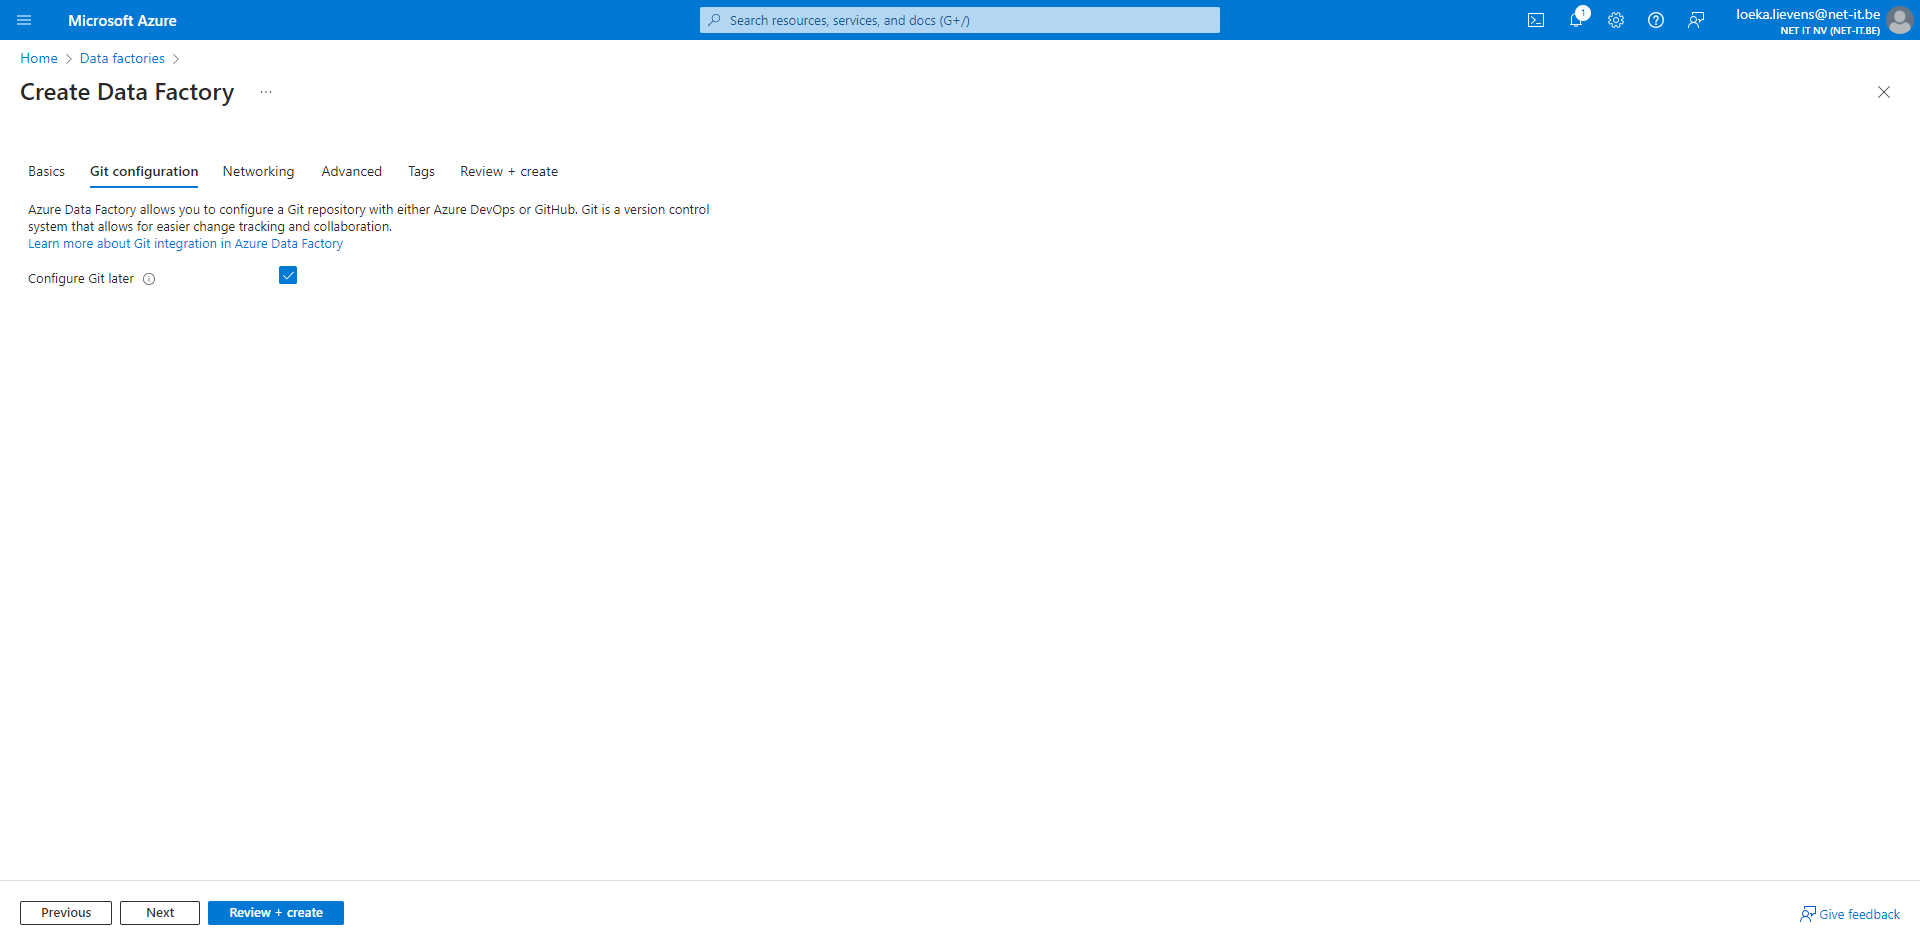
\includegraphics[width=1\textwidth]{./graphics/adf/initial_2.png}
%\end{center}
%
%Door bij de vorige stap op next te klikken kunnen we er voor kiezen om een Git configuratie te gaan toevoegen. Dit zullen we pas later gaan doen. Klik nu op `Review + create` om de data factory aan te maken.
%
%\begin{center}
%    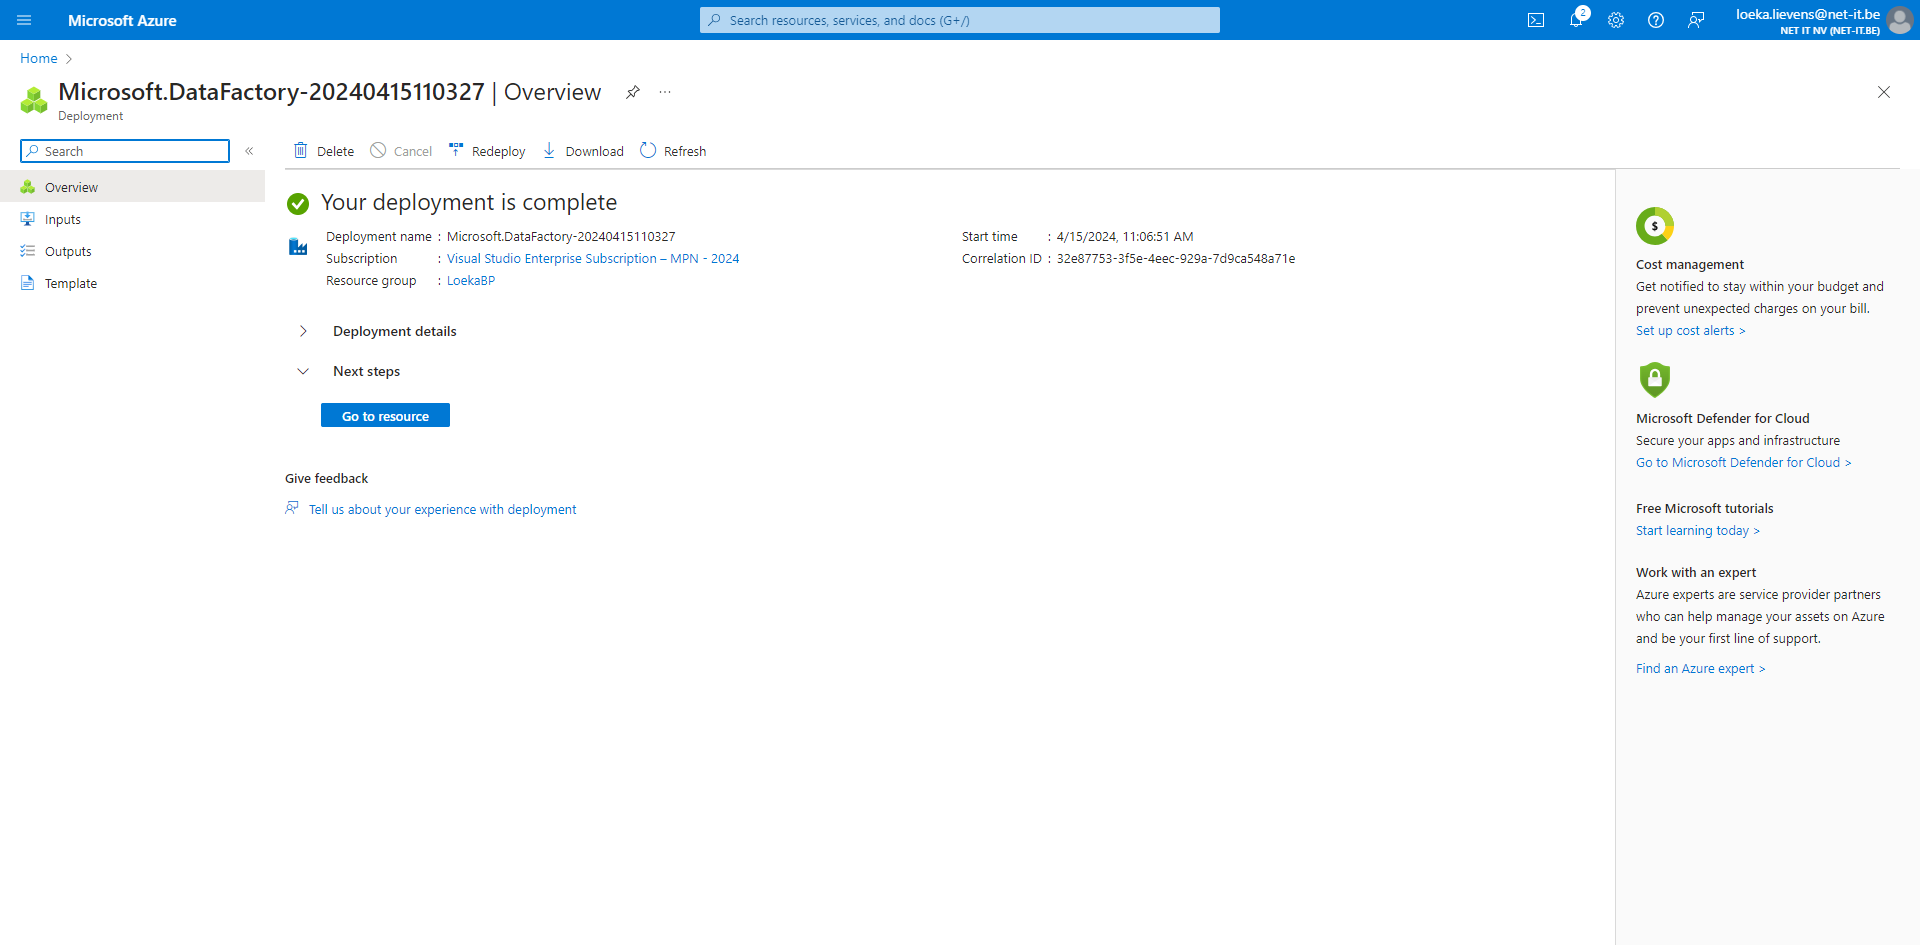
\includegraphics[width=1\textwidth]{./graphics/adf/deployment_complete.png}
%\end{center}
%
%Wanneer onze deployment complete is kunnen we naar onze resource gaan door op `Go to resource` te klikken.
%
%\begin{center}
%    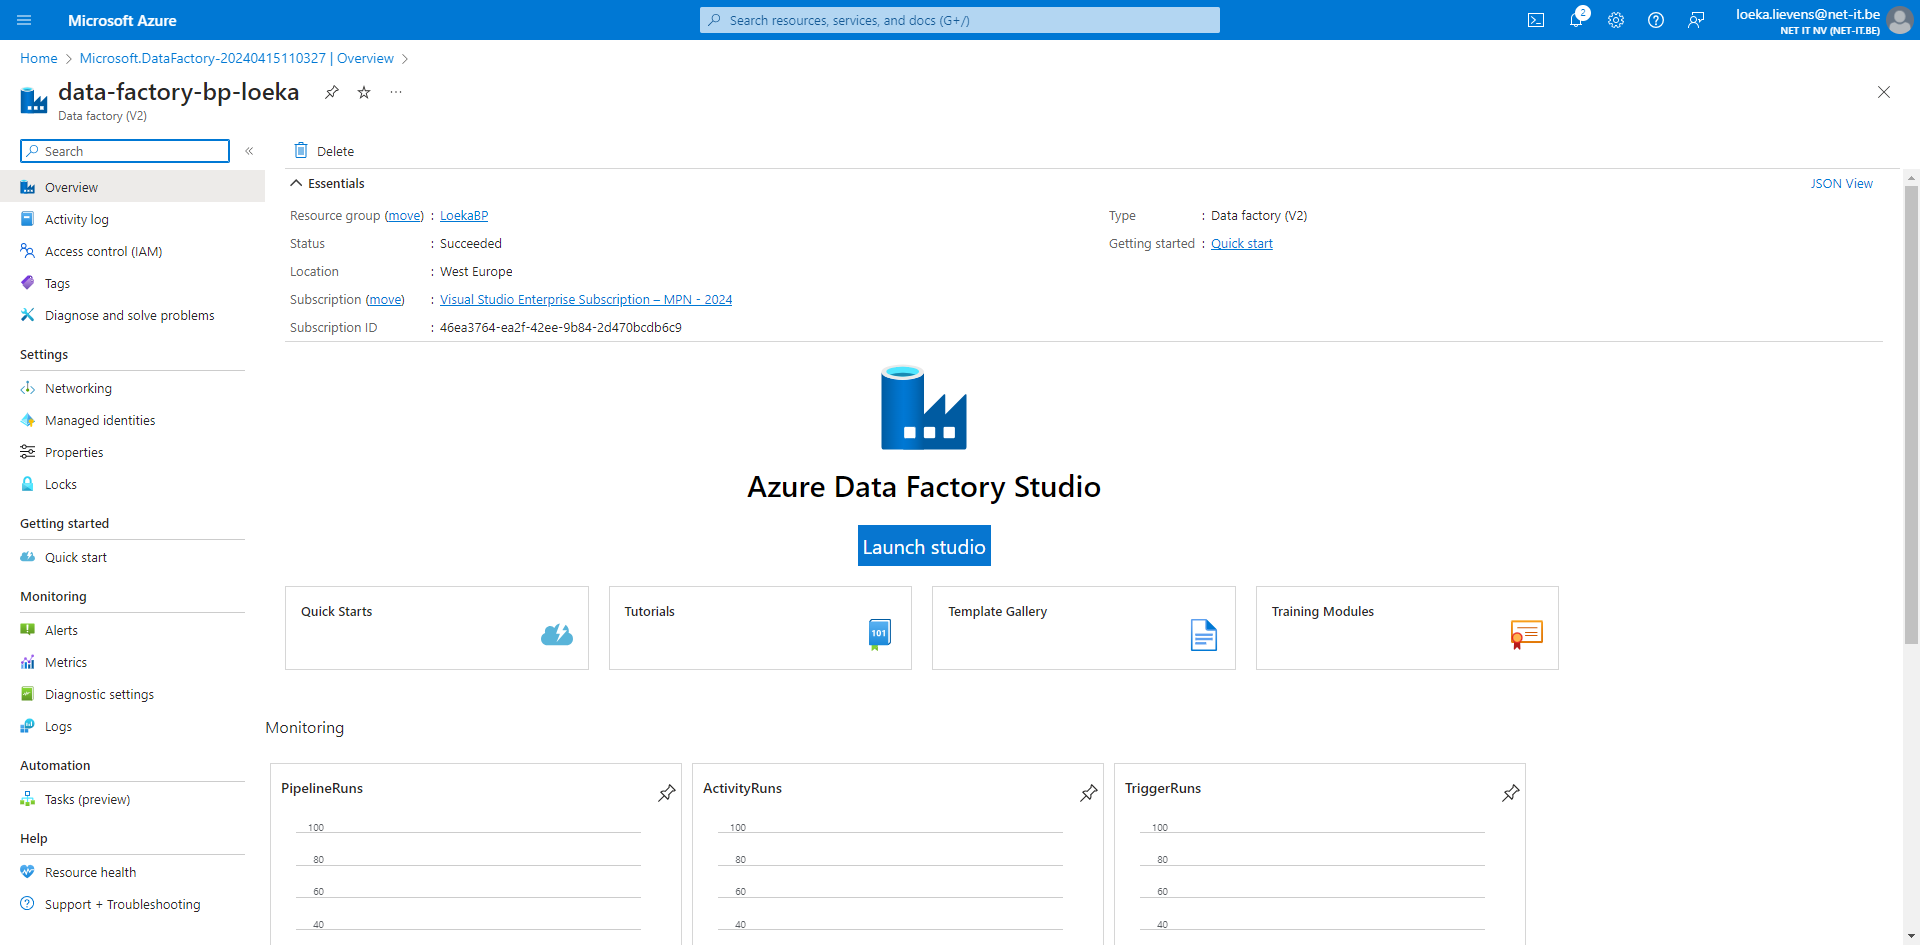
\includegraphics[width=1\textwidth]{./graphics/adf/launch_adf.png}
%\end{center}
%
%Klik nu op `Launch studio` om naar Azure Data Factory Studio te gaan.
%
%\subsubsection{Koppeling met Git}
%
%\begin{center}
%    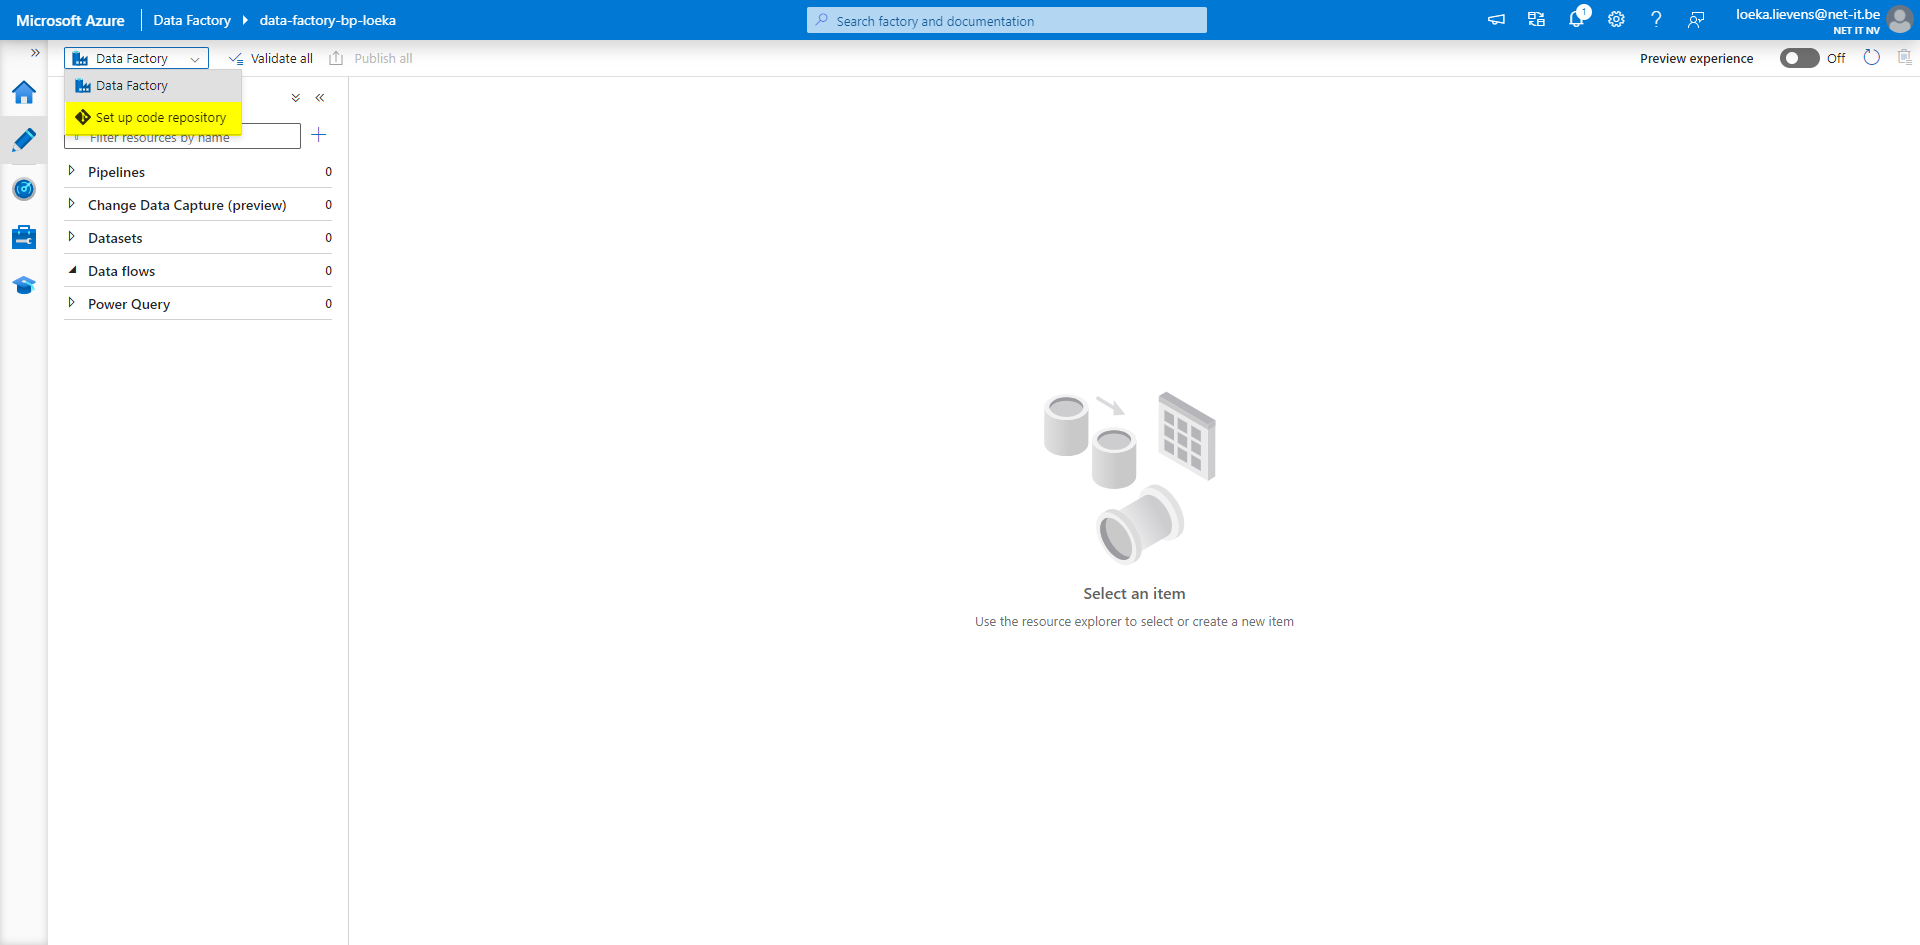
\includegraphics[width=1\textwidth]{./graphics/adf/setup_repository.png}
%\end{center}
%
%Voor we onze ETL gaan implementeren zullen we eerst onze data factory koppelen met Git.
%
%\begin{center}
%    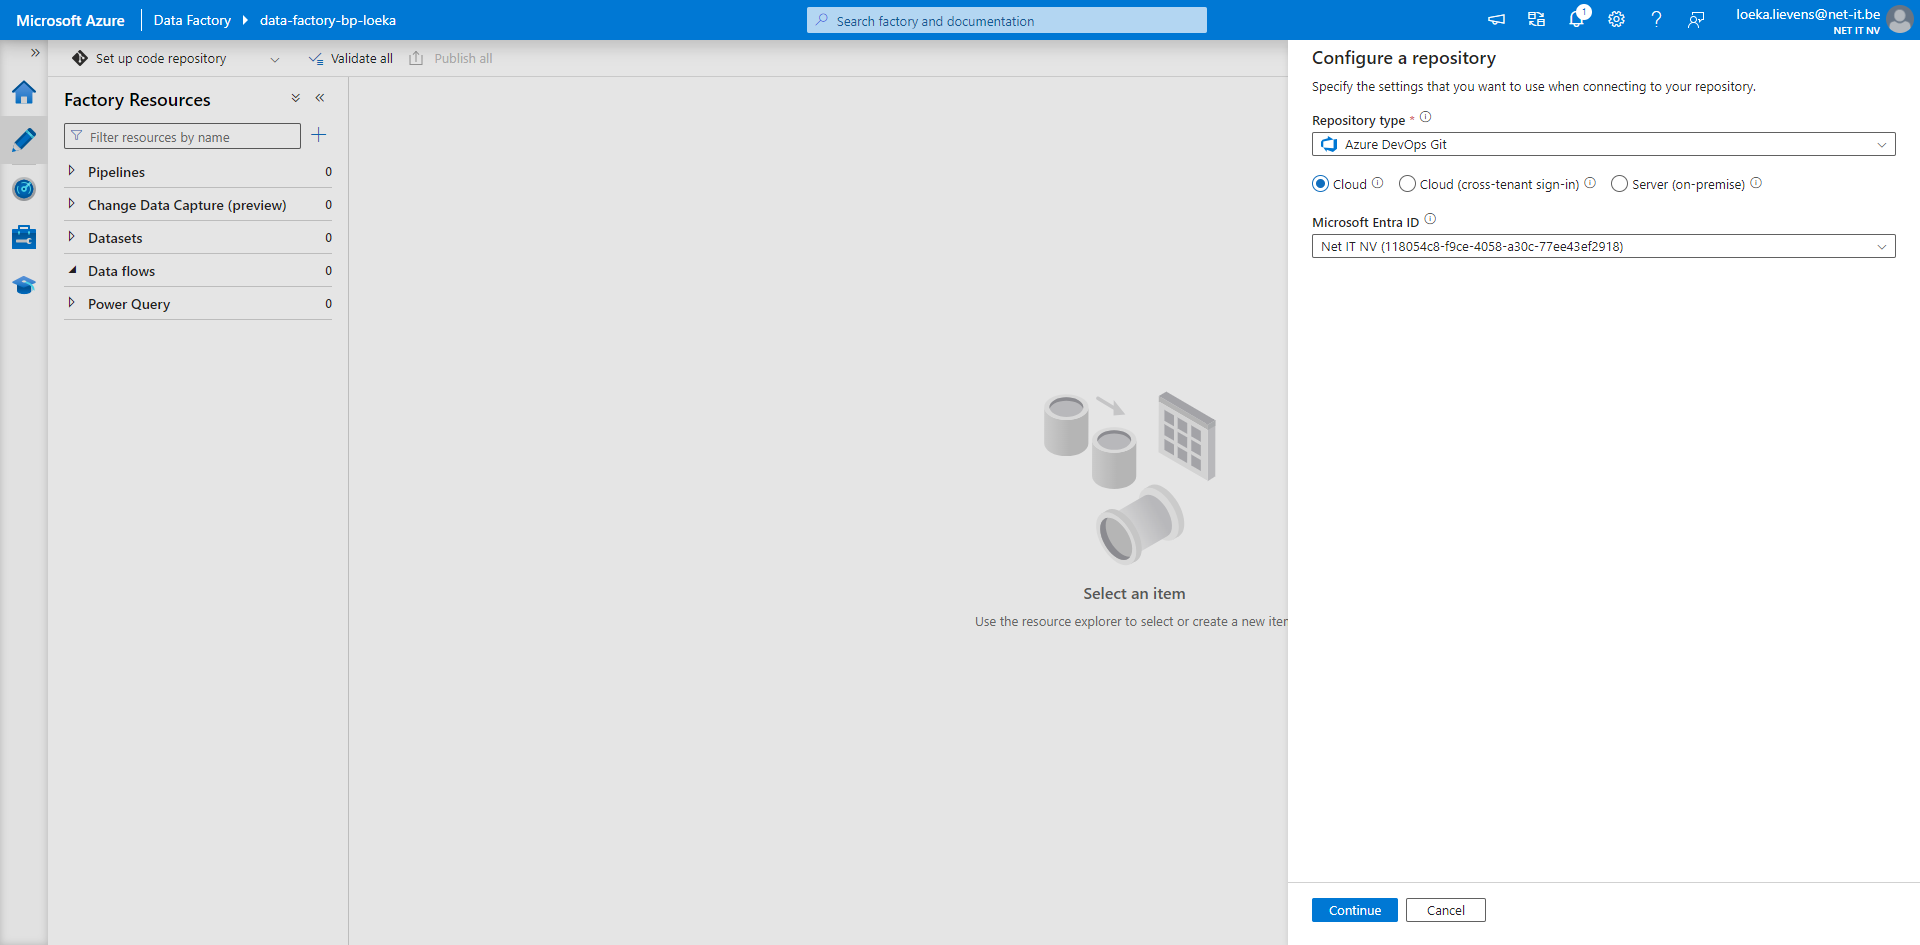
\includegraphics[width=1\textwidth]{./graphics/adf/setup_repository_2.png}
%\end{center}
%
%\begin{center}
%    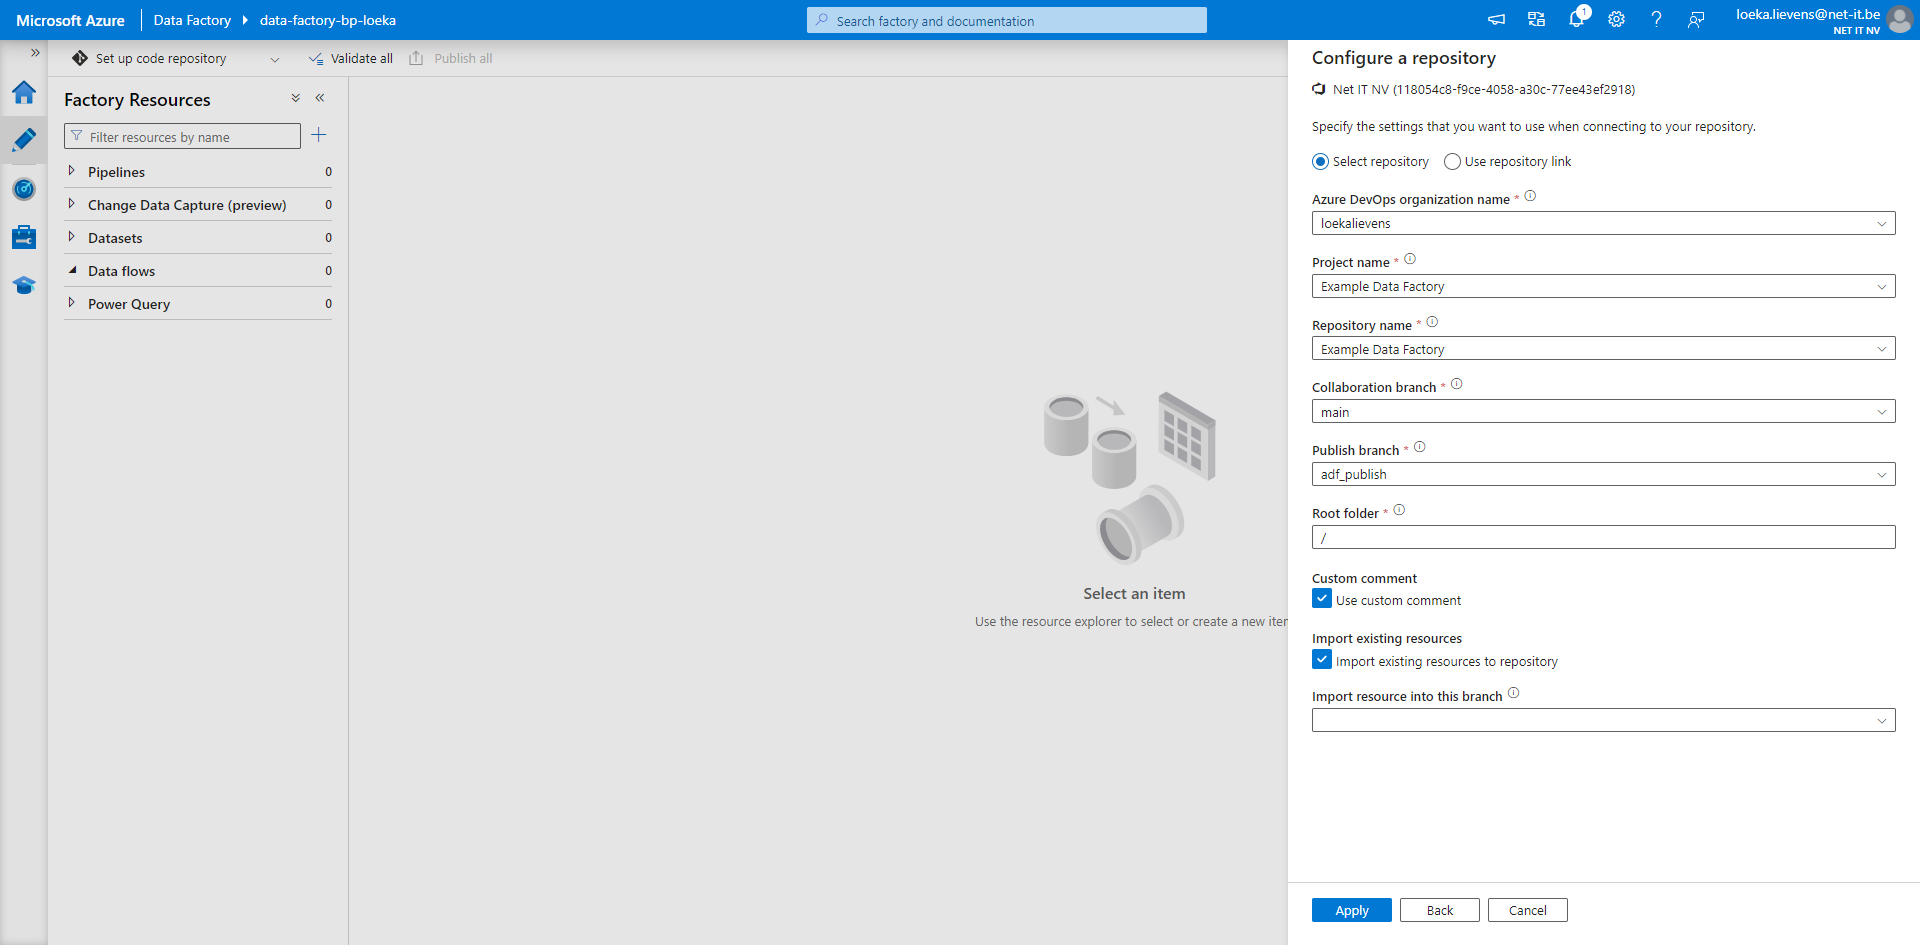
\includegraphics[width=1\textwidth]{./graphics/adf/setup_repository_3.png}
%\end{center}
%
%Binnen Net IT wordt er gewerkt met Azure DevOps Git.
%
%\subsubsection{Het toevoegen van een source}
%
%Telkens wanneer we een source tabel zullen gaan toevoegen zal dit op dezelfde manier gebeuren.
%
%\begin{center}
%    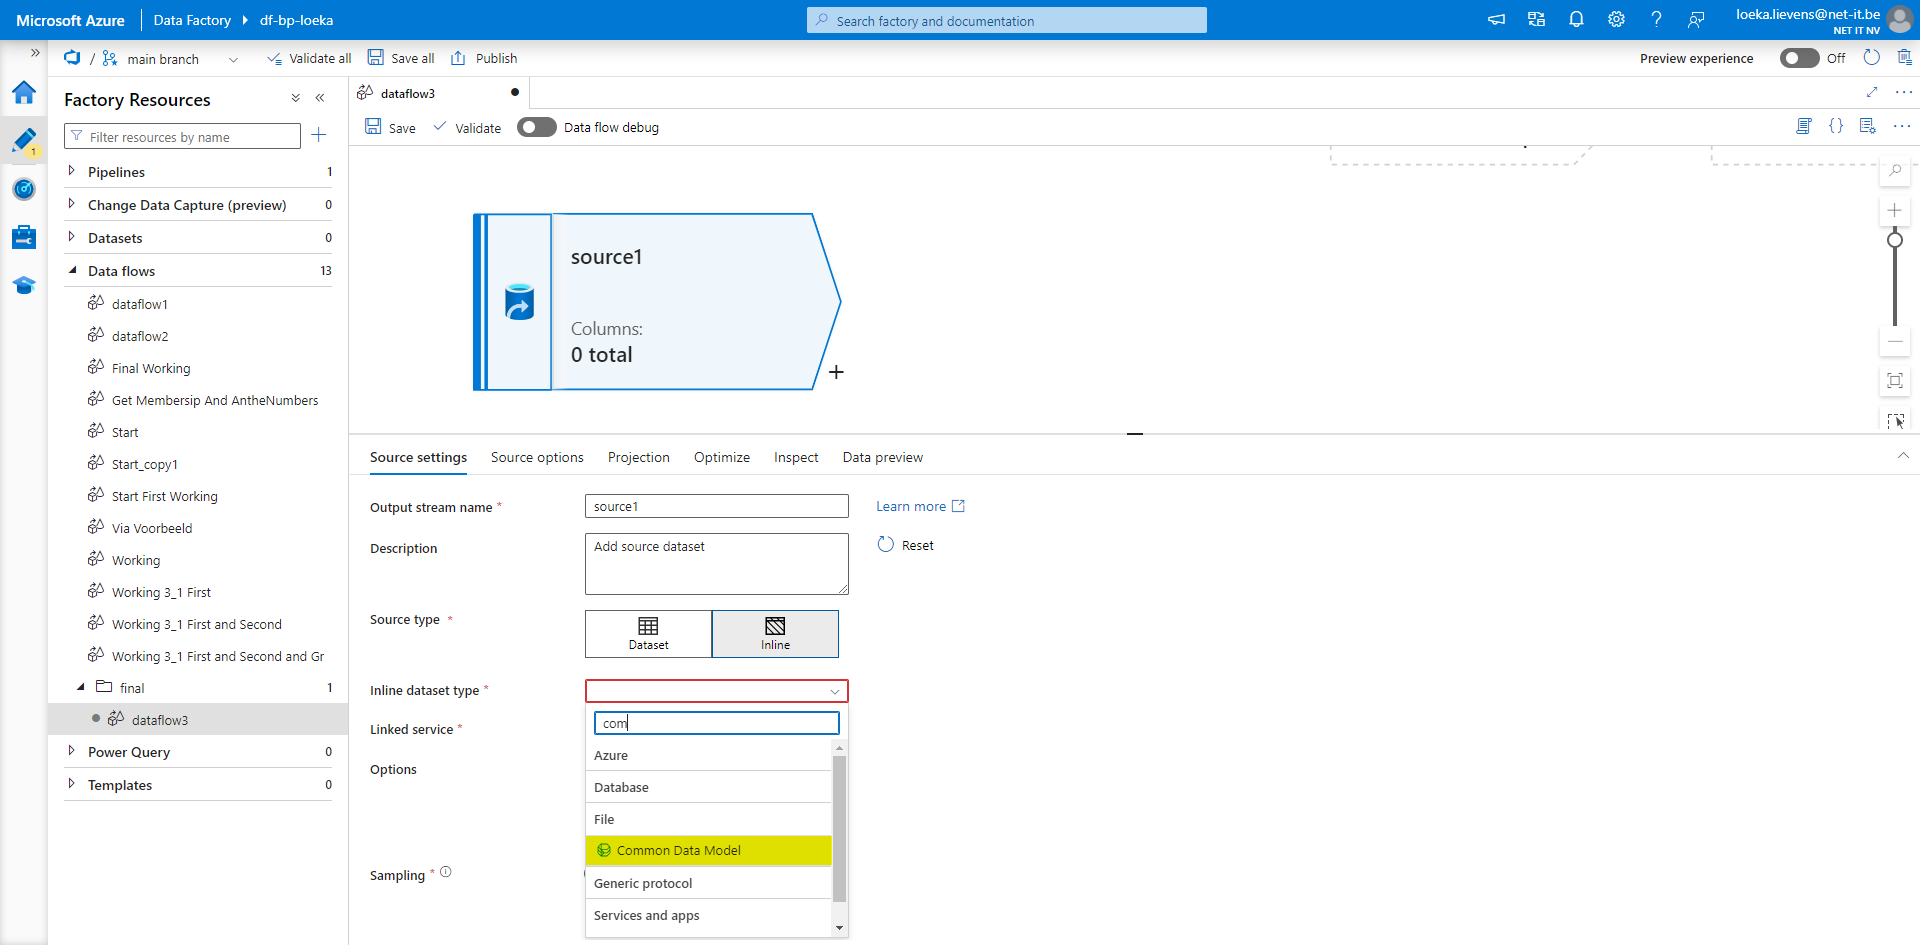
\includegraphics[width=1\textwidth]{./graphics/adf/source_table_1.png}
%\end{center}
%
%Als source type zal er steeds gekozen worden voor inline. Dit doordat we slechts één enkele dataflow zullen gaan aanmaken en geen gedeelde datasets nodig hebben. Als type voor de linked service kiezen we voor Common Data Model.
%
%\begin{center}
%    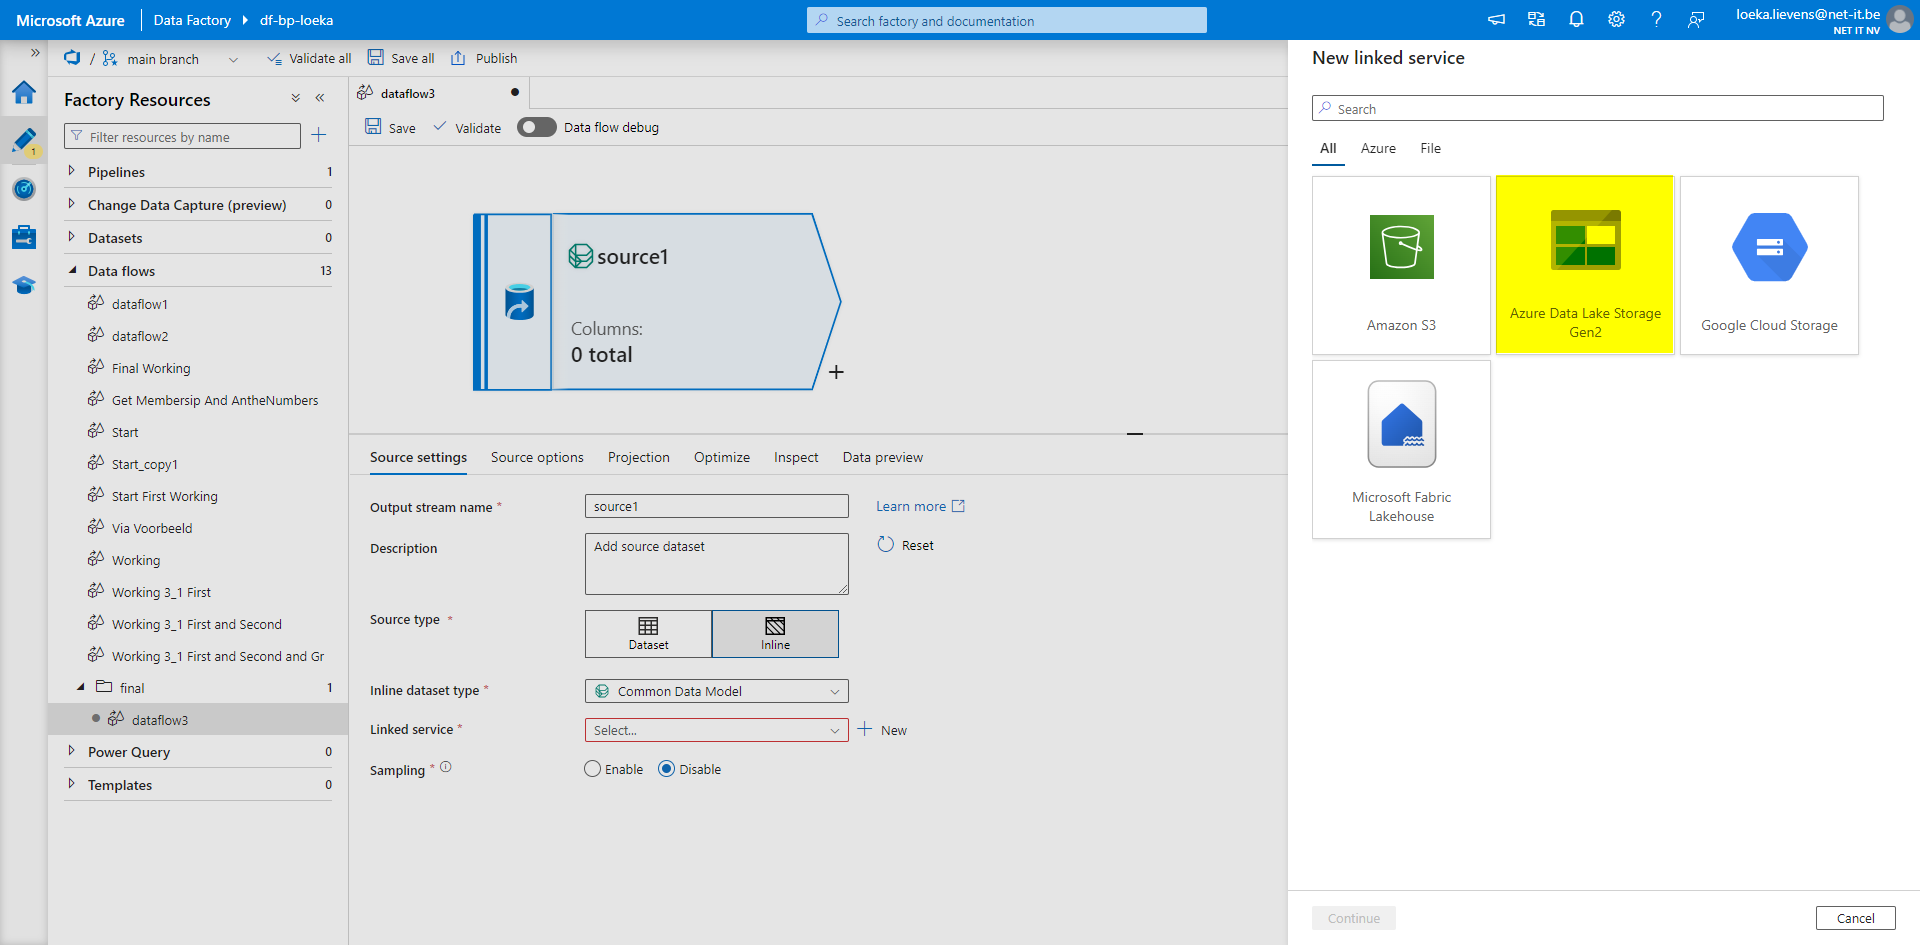
\includegraphics[width=1\textwidth]{./graphics/adf/source_table_2.png}
%\end{center}
%
%Er zal éénmalig een Linked Service aangemaakt moeten worden. Hierbij kiezen we voor Azure Data Lake Storage Gen2.
%
%\begin{center}
%    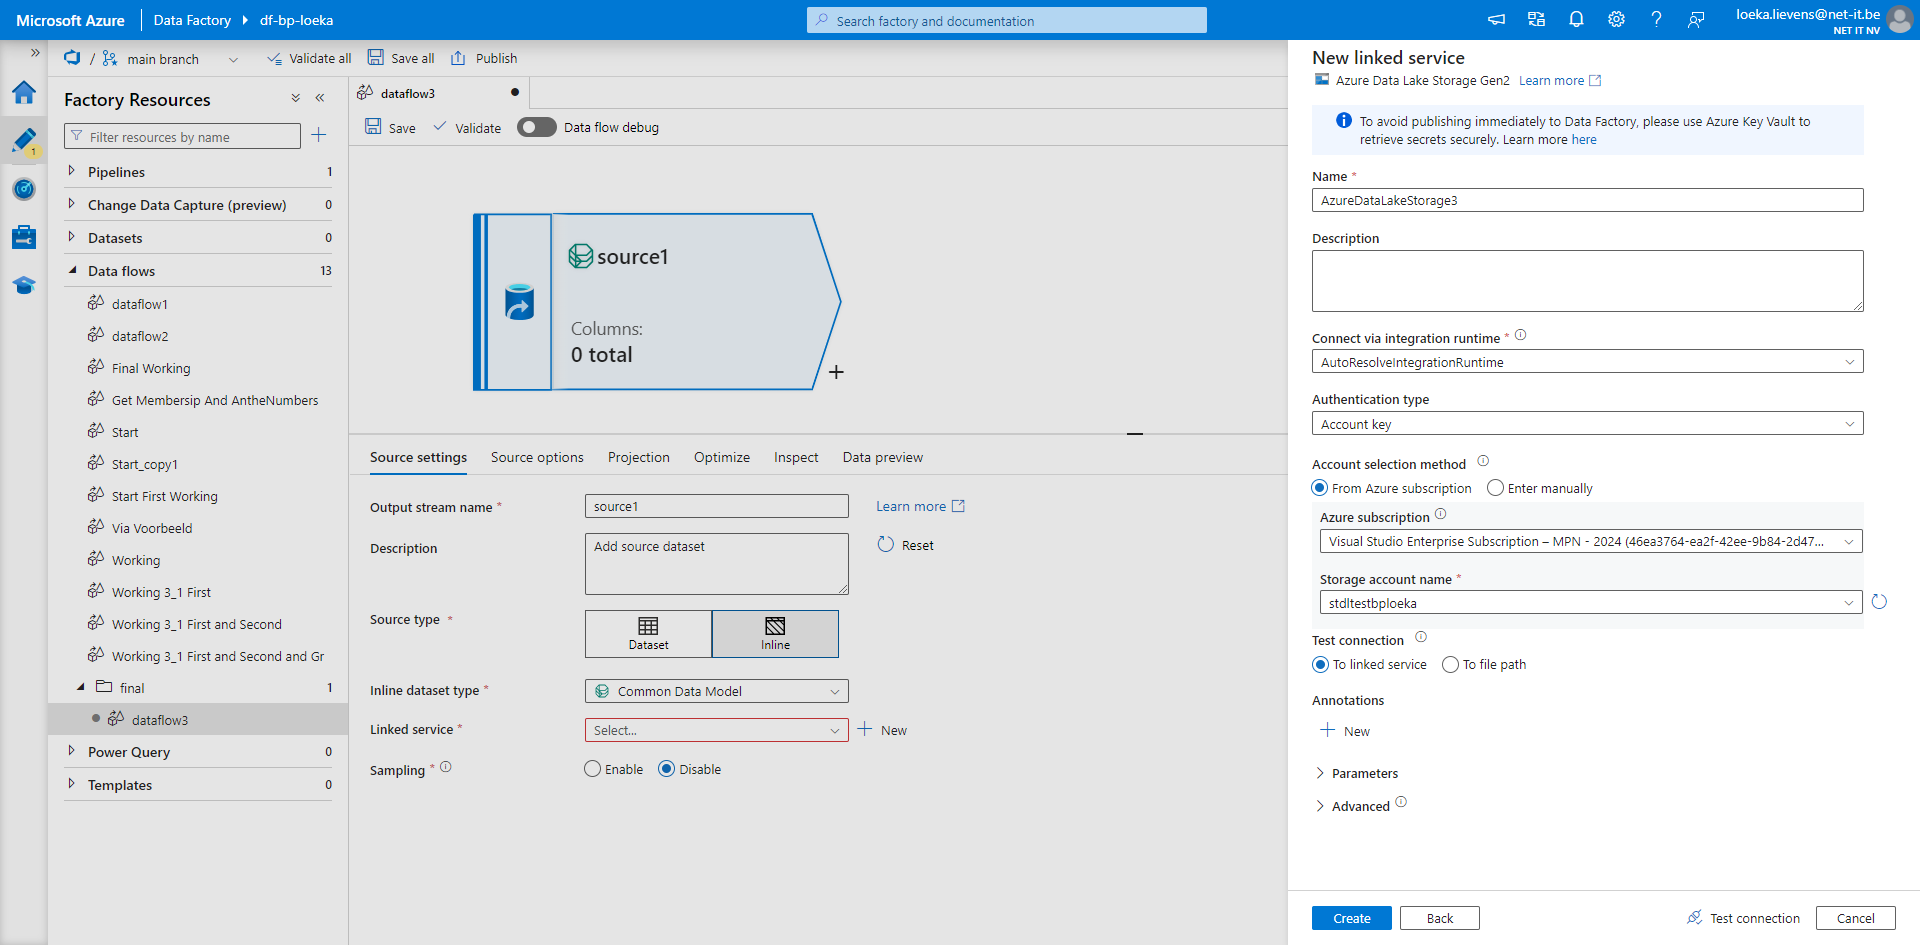
\includegraphics[width=1\textwidth]{./graphics/adf/source_table_3.png}
%\end{center}
%
%We kunnen makkelijk gaan koppelen met de juiste data lake door een Azure Subscription en Storage account name aan te duiden. Door op `Test connection` te klikken kunnen we kijken of de connectie met data lake is gelukt. Door op `Create` te klikken hebben we nu een Linked Service die steeds bij elke Source gebruikt kan worden.
%
%\begin{center}
%    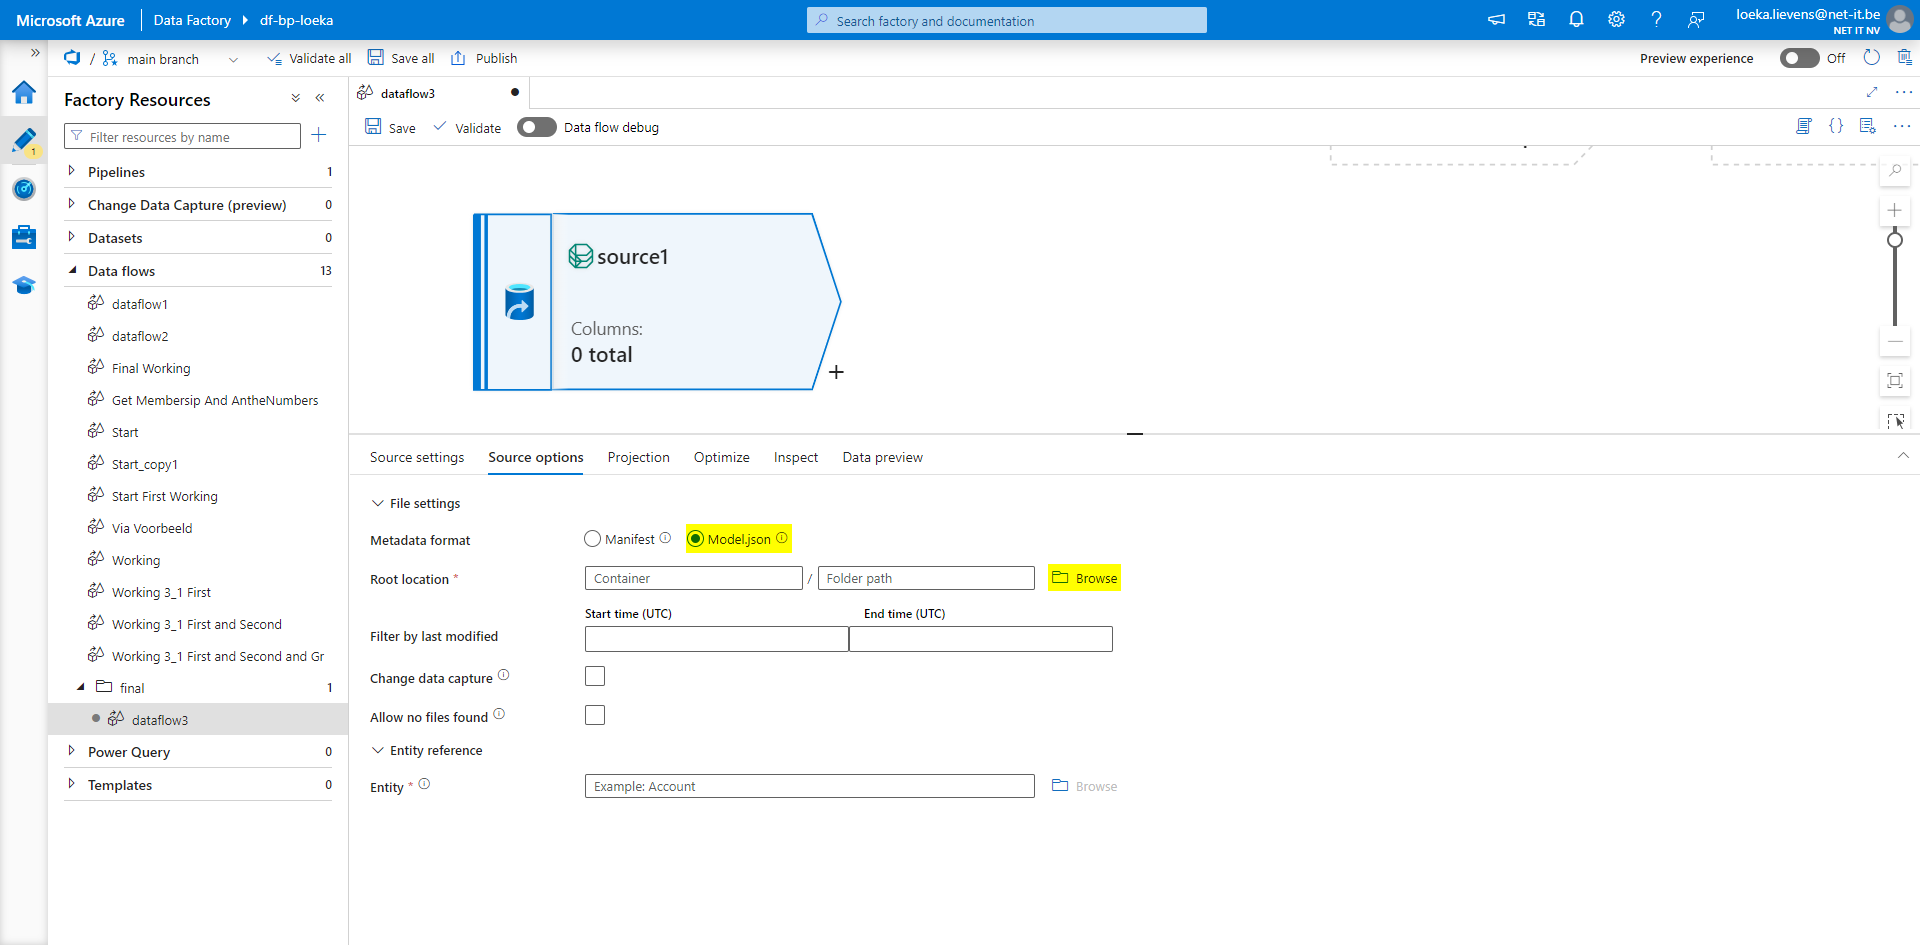
\includegraphics[width=1\textwidth]{./graphics/adf/source_table_4.png}
%\end{center}
%
%Door naar `Source options` te gaan kunnen we `Model.json` gaan aanduiden. Door op `Browse` te klikken kunnen we aanduiden waar het Model.json bestand te vinden is in data lake.
%
%\begin{center}
%    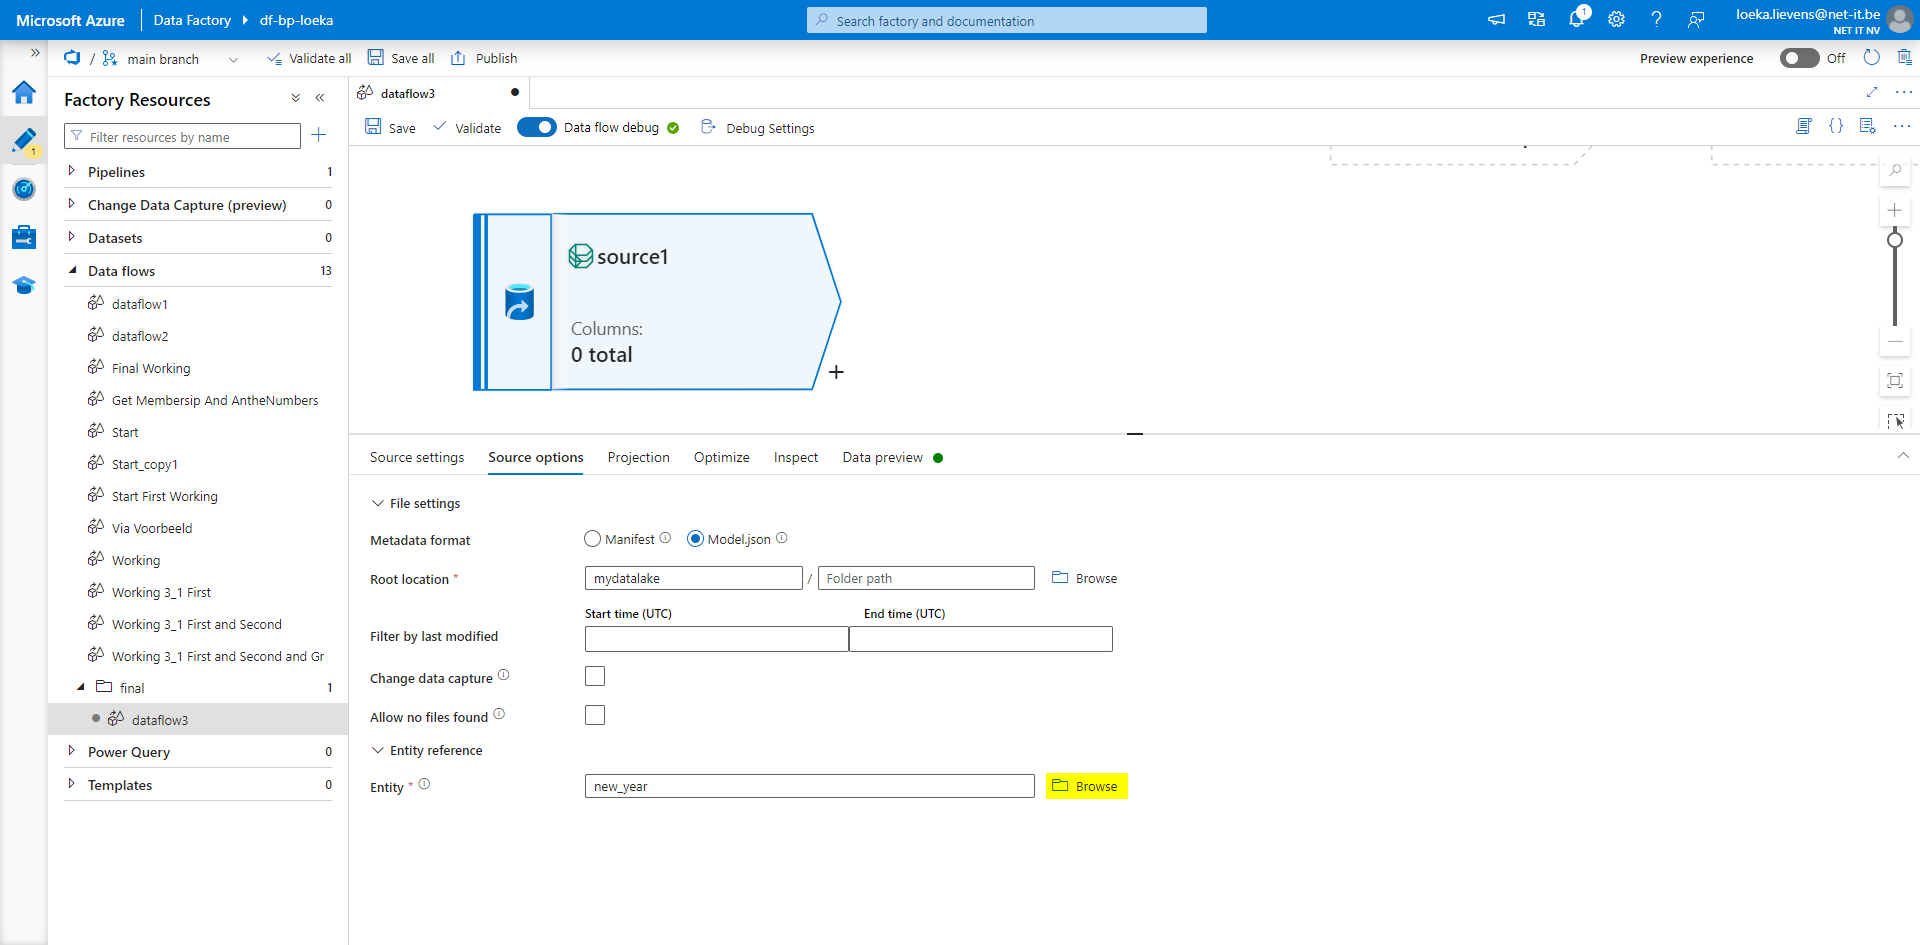
\includegraphics[width=1\textwidth]{./graphics/adf/source_table_5.png}
%\end{center}
%
%Naast `Entity` kunnen we nu op `Browse` klikken om de gewenste entity te gaan importeren. Let op: hier voor zal Data flow debug aan moeten staan.
%
%\begin{center}
%    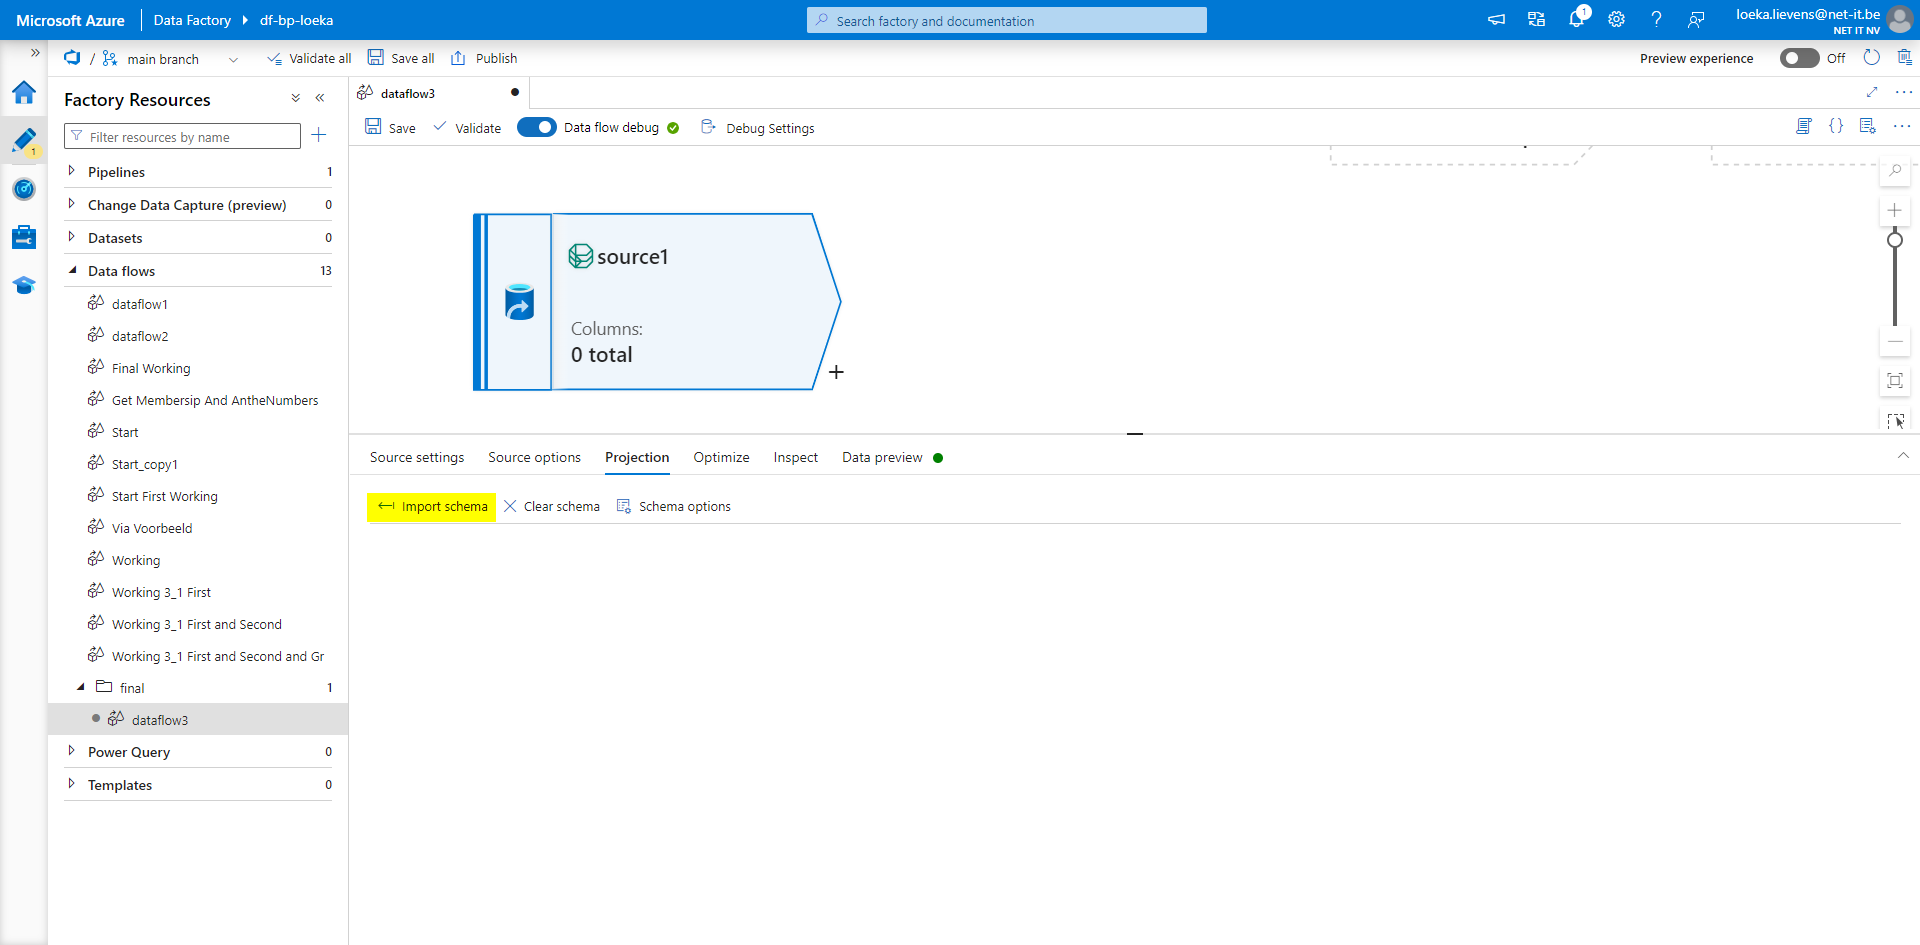
\includegraphics[width=1\textwidth]{./graphics/adf/source_table_6.png}
%\end{center}
%
%Door naar `Projection` te gaan kunnen we nu op `Import schema` klikken.
%
%\begin{center}
%    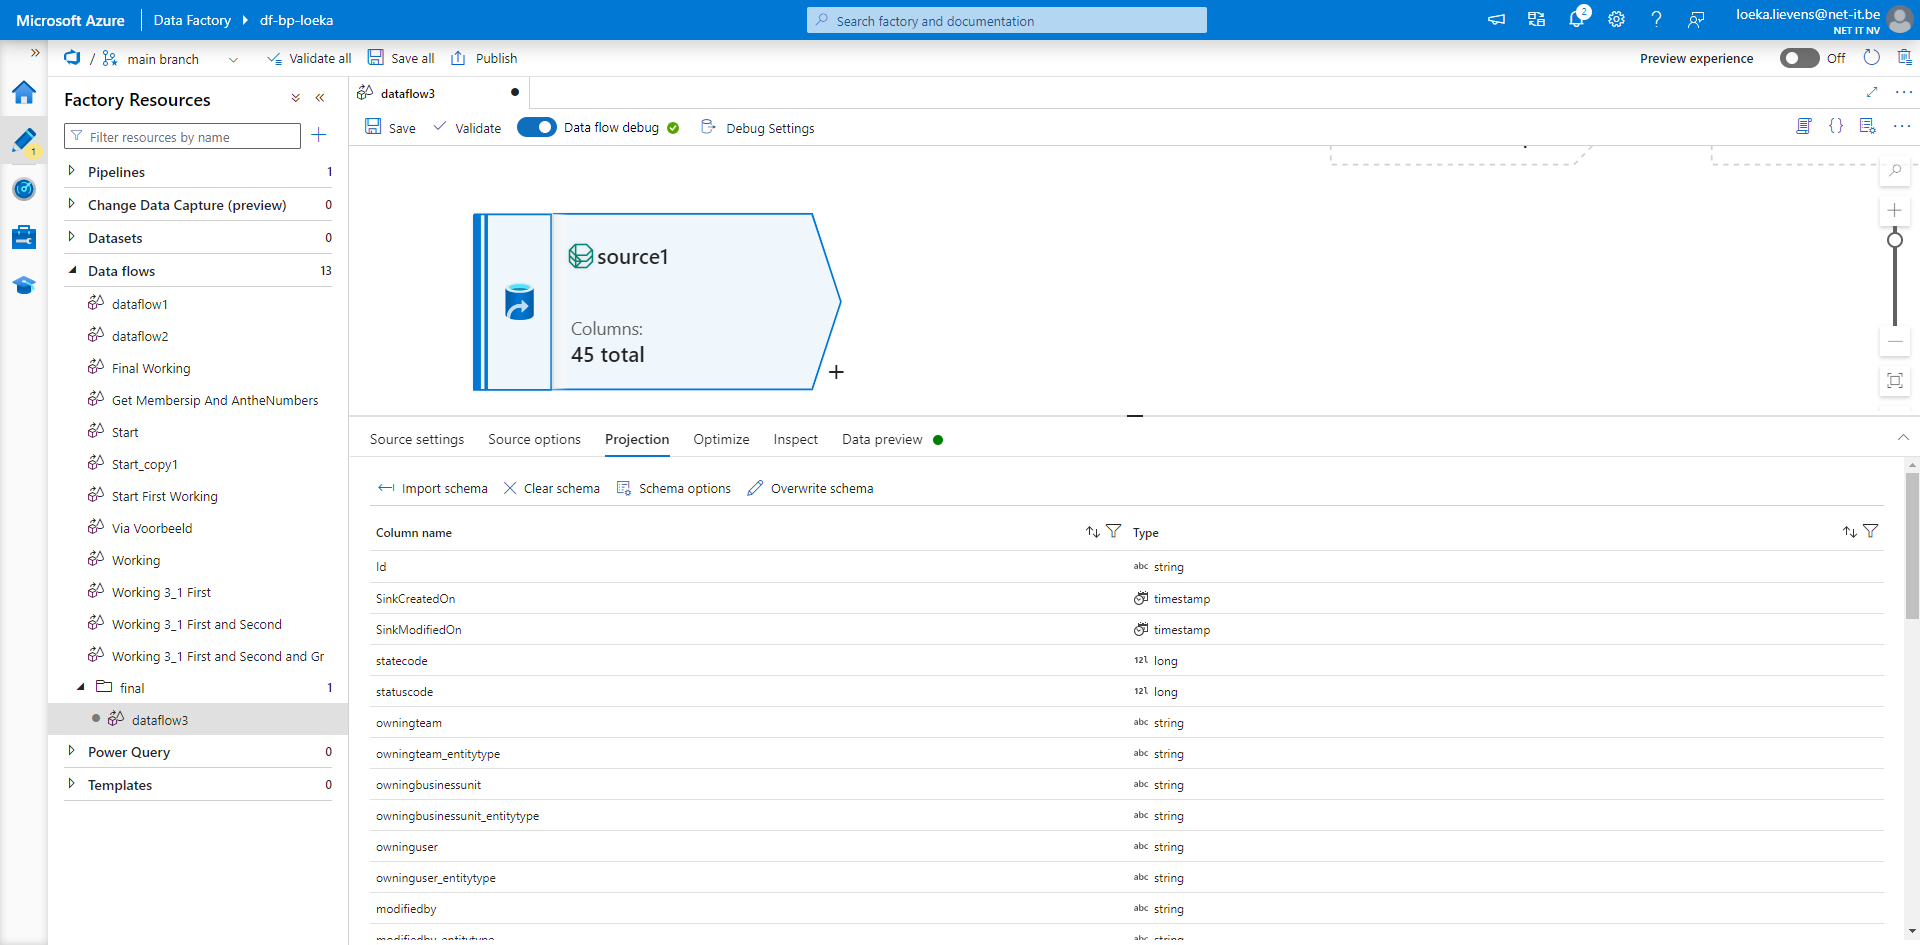
\includegraphics[width=1\textwidth]{./graphics/adf/source_table_7.png}
%\end{center}
%
%De foto hierboven toont een voorbeeld van een geïmporteerd schema.
%
%\begin{center}
%    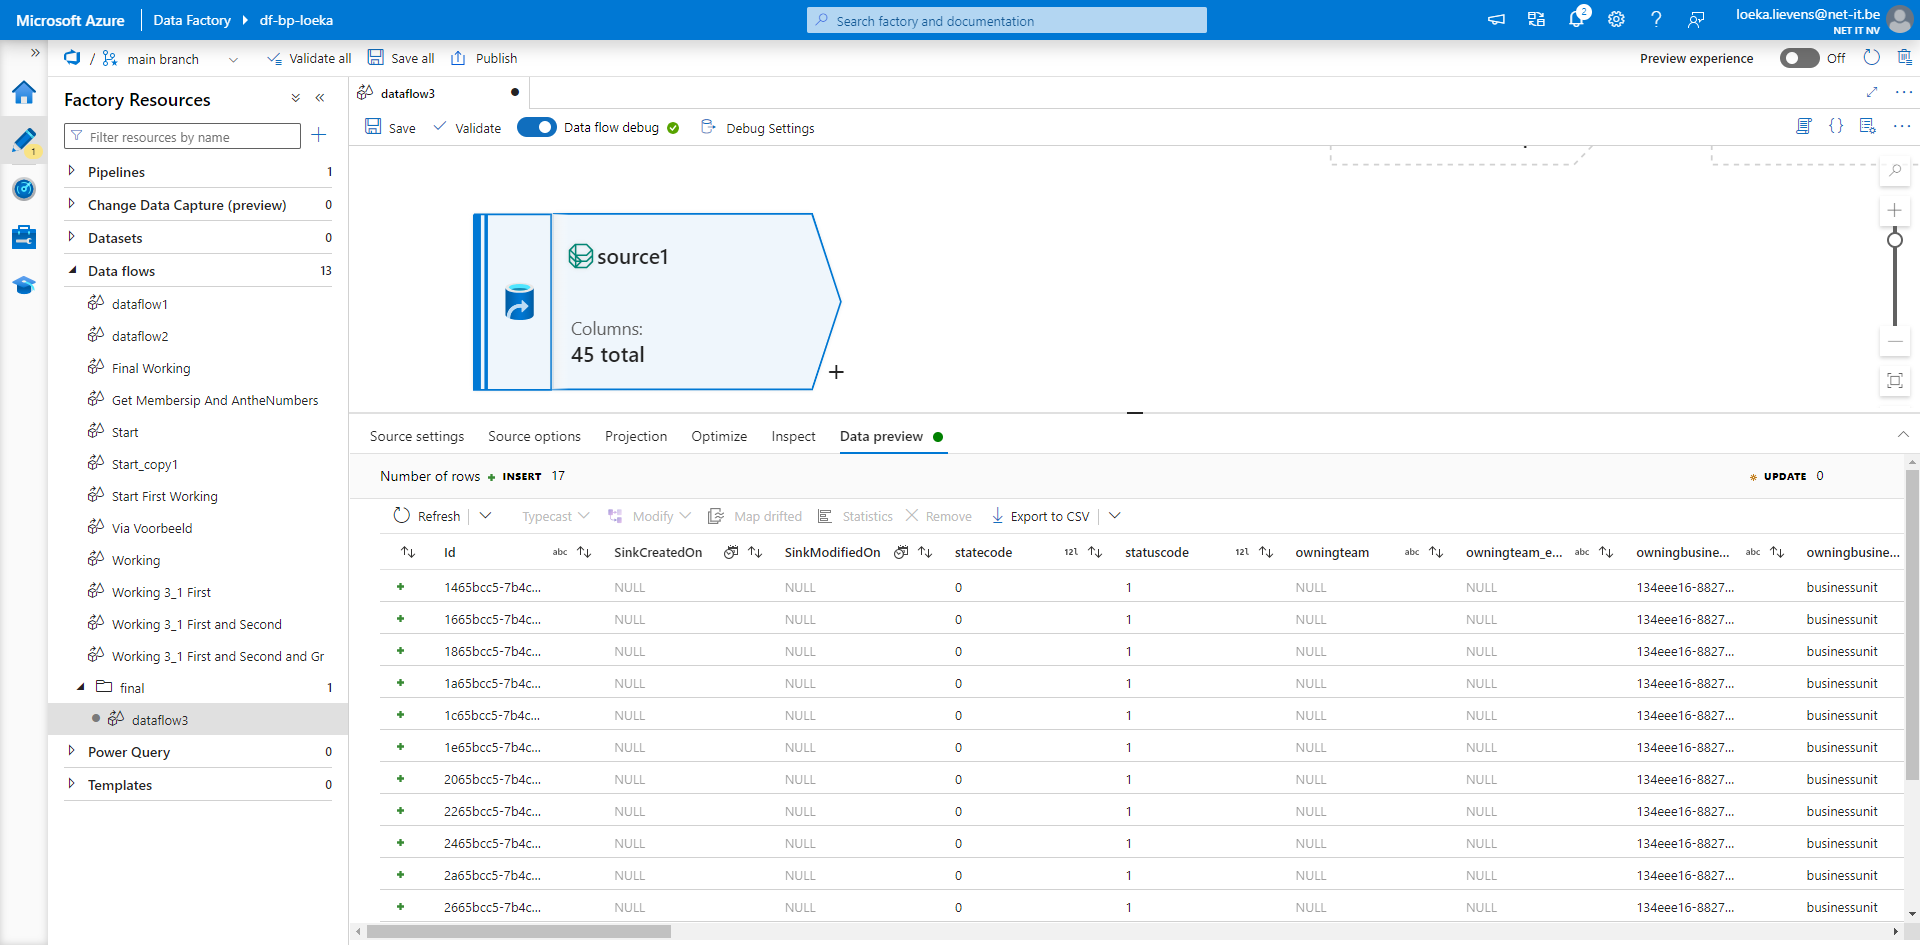
\includegraphics[width=1\textwidth]{./graphics/adf/source_table_8.png}
%\end{center}
%
%Wanneer we naar `Data preview` gaan kunnen we een preview zien van de data uit de gekozen tabel.
%
%\subsubsection{Implementatie ETL}
%
%\begin{center}
%    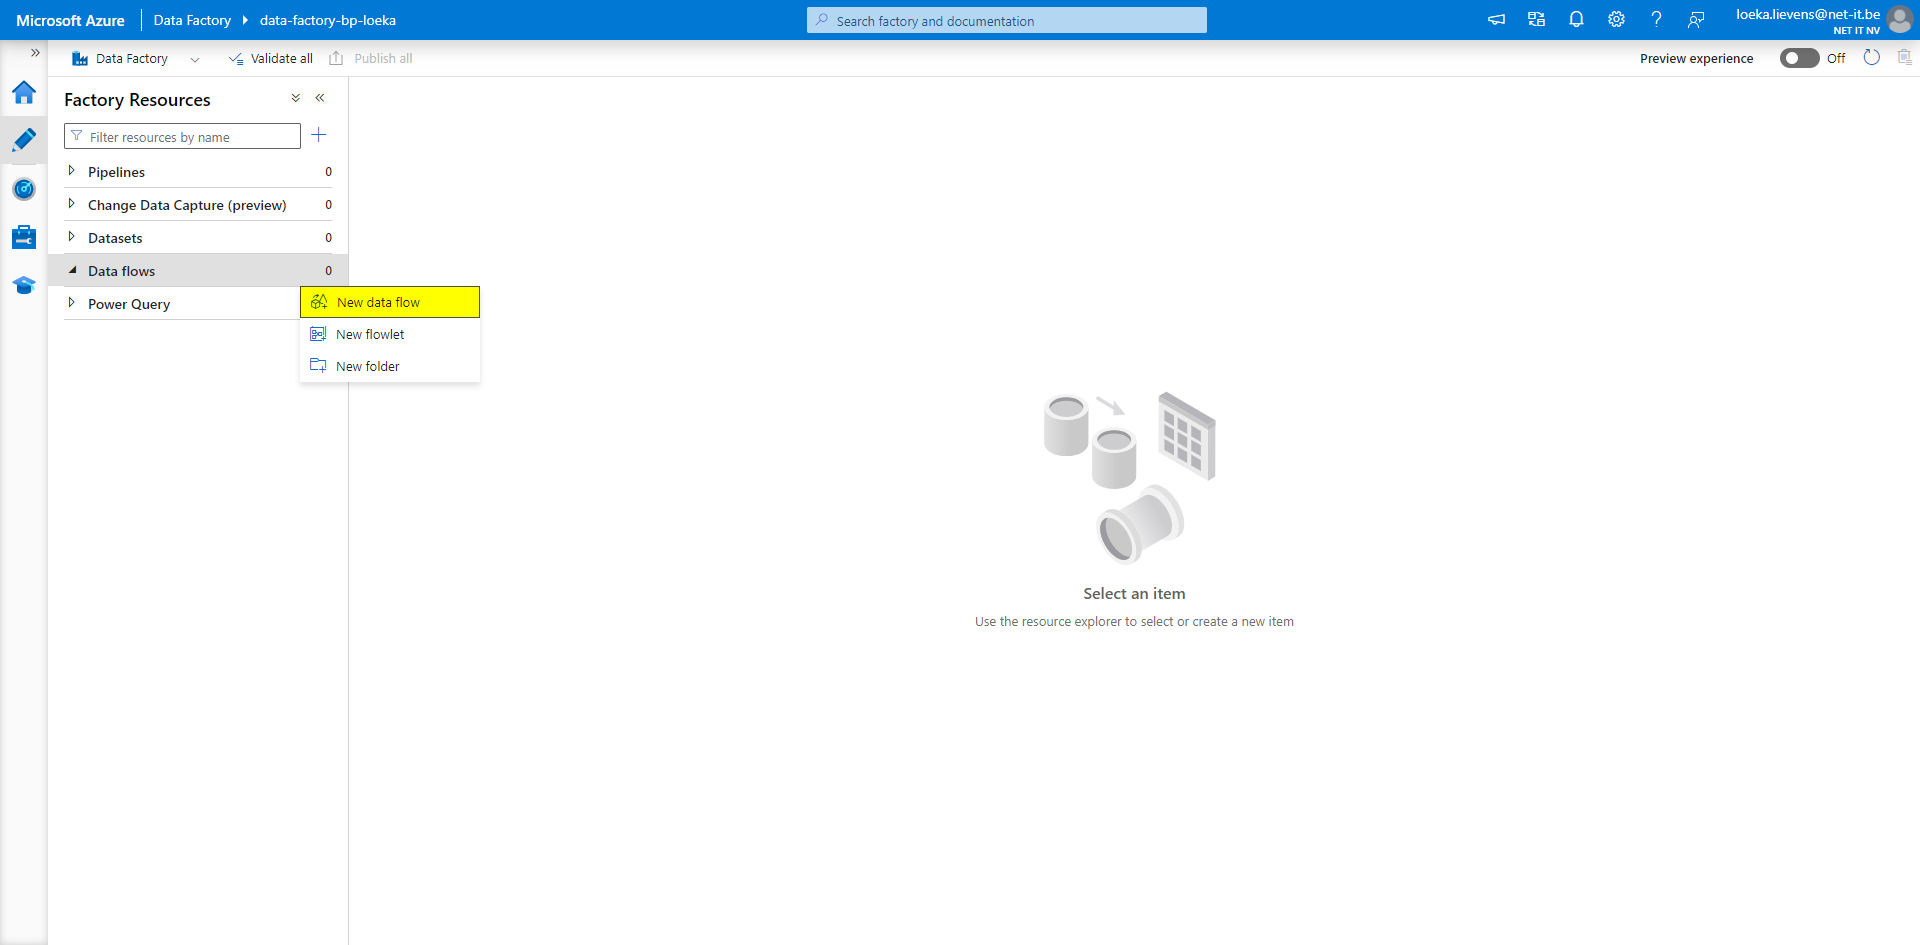
\includegraphics[width=1\textwidth]{./graphics/adf/dataflow.png}
%\end{center}
%
%Voor het implementeren van onze ETL gaan we een nieuwe dataflow gaan aanmaken.
%
%\paragraph{\texttt{Tabel new\_person}}
%
%\begin{center}
%    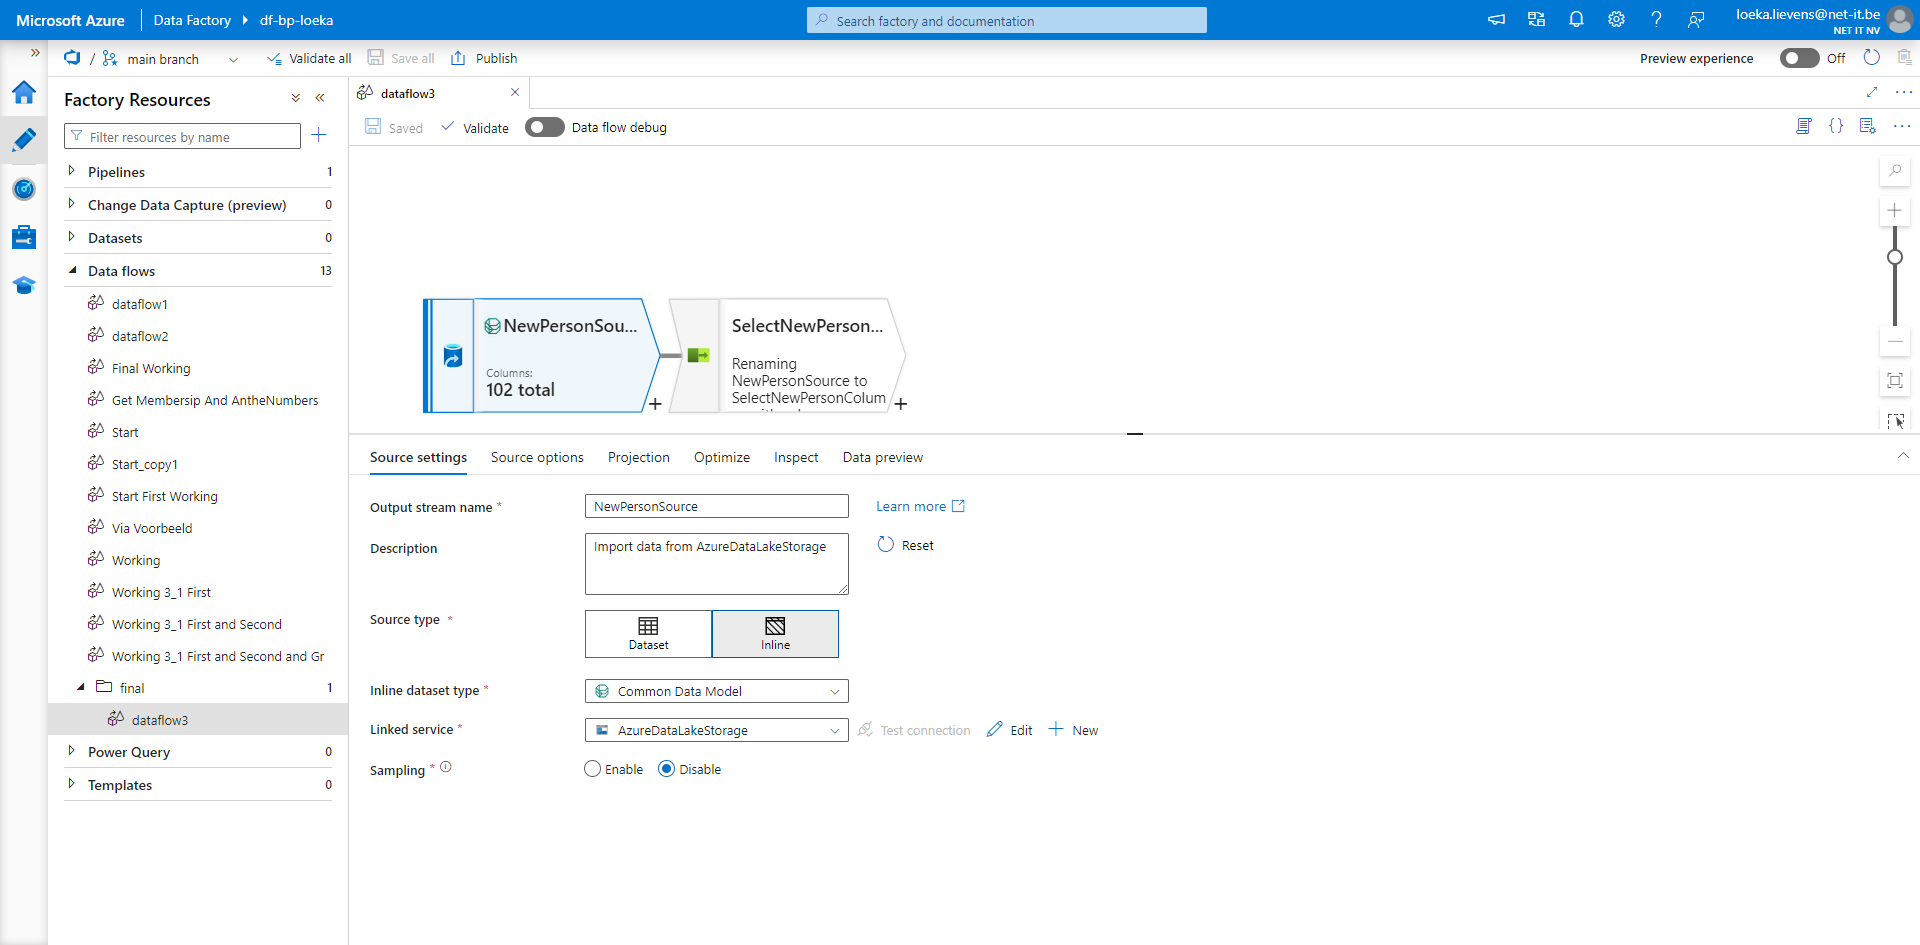
\includegraphics[width=1\textwidth]{./graphics/adf/new_person_source.png}
%\end{center}
%
%\texttt{Er wordt een source toegevoegd voor de tabel new\_person.}
%
%\begin{center}
%    \includegraphics[width=1\textwidth]{./graphics/adf/new_person_select.png}
%\end{center}
%
%\texttt{De nodige kolommen worden geselecteerd en hernoemt met de prefix `p\_`.}
%
%\paragraph{\texttt{Tabel new\_bankaccount}}
%
%\begin{center}
%    \includegraphics[width=1\textwidth]{./graphics/adf/new_bankaccount_source.png}
%\end{center}
%
%\texttt{Er wordt een source toegevoegd voor de tabel new\_bankaccount.}
%
%\begin{center}
%    \includegraphics[width=1\textwidth]{./graphics/adf/new_bankaccount_select.png}
%\end{center}
%
%\texttt{De nodige kolommen worden geselecteerd en hernoemt met de prefix `ba\_`.}
%
%\paragraph{\texttt{Tabel new\_year}}
%
%\begin{center}
%    \includegraphics[width=1\textwidth]{./graphics/adf/new_year_source.png}
%\end{center}
%
%\texttt{Er wordt een source toegevoegd voor de tabel new\_year.}
%
%\begin{center}
%    \includegraphics[width=1\textwidth]{./graphics/adf/new_year_select.png}
%\end{center}
%
%\texttt{De nodige kolommen worden geselecteerd en hernoemt met de prefix `ny\_`.}
%
%\paragraph{\texttt{Tabel new\_group}}
%
%\begin{center}
%    \includegraphics[width=1\textwidth]{./graphics/adf/new_group_source.png}
%\end{center}
%
%\texttt{Er wordt een source toegevoegd voor de tabel new\_group.}
%
%\begin{center}
%    \includegraphics[width=1\textwidth]{./graphics/adf/new_group_select.png}
%\end{center}
%
%\texttt{De nodige kolommen worden geselecteerd en hernoemt met de prefix `ng\_`.}
%
%\paragraph{\texttt{Tabel new\_organizationyear}}
%
%\begin{center}
%    \includegraphics[width=1\textwidth]{./graphics/adf/new_organizationyear_source.png}
%\end{center}
%
%\texttt{Er wordt een source toegevoegd voor de tabel new\_organizationyear.}
%
%\begin{center}
%    \includegraphics[width=1\textwidth]{./graphics/adf/new_organizationyear_select.png}
%\end{center}
%
%\texttt{De nodige kolommen worden geselecteerd en hernoemt met de prefix `noy\_`.}
%
%\begin{center}
%    \includegraphics[width=1\textwidth]{./graphics/adf/new_organizationyear_lookup.png}
%\end{center}
%
%\texttt{De tabel new\_group wordt gejoind met een lookup aan de hand van id.}
%
%% TODO: Link naar juiste foto?
%
%\begin{center}
%    \includegraphics[width=1\textwidth]{./graphics/adf/new_organizationyear_final.png}
%\end{center}
%
%\texttt{We selecteren alle kolommen behalve de kolom met naam ng\_id aangezien deze steeds hetzelfde zal zijn als noy\_new\_groupid.}
%
%\paragraph{\texttt{Tabel new\_membership}}
%
%\begin{center}
%    \includegraphics[width=1\textwidth]{./graphics/adf/new_membership_source.png}
%\end{center}
%
%\texttt{Er wordt een source toegevoegd voor de tabel new\_membership.}
%
%\begin{center}
%    \includegraphics[width=1\textwidth]{./graphics/adf/new_membership_select.png}
%\end{center}
%
%\texttt{De nodige kolommen worden geselecteerd en hernoemt met de prefix `membership\_`.}
%
%\begin{center}
%    \includegraphics[width=1\textwidth]{./graphics/adf/new_membership_filter_1.png}
%\end{center}
%
%\begin{center}
%    \includegraphics[width=1\textwidth]{./graphics/adf/new_membership_filter_2.png}
%\end{center}
%
%\texttt{De membership records worden gefilterd aan de hand van `new\_f30statuscode`, `new\_memberstatuscode` en `new\_aclvbstatuscode`.}
%
%\begin{center}
%    \includegraphics[width=1\textwidth]{./graphics/adf/new_membership_join_1.png}
%\end{center}
%
%\texttt{De tabel new\_group wordt gejoind aan de hand van id.}
%
%\begin{center}
%    \includegraphics[width=1\textwidth]{./graphics/adf/new_membership_join_2.png}
%\end{center}
%
%\texttt{De tabel new\_year wordt gejoind aan de hand van id.}
%
%\begin{center}
%    \includegraphics[width=1\textwidth]{./graphics/adf/new_membership_secondselect_1.png}
%\end{center}
%
%\begin{center}
%    \includegraphics[width=1\textwidth]{./graphics/adf/new_membership_secondselect_2.png}
%\end{center}
%
%\texttt{De kolom `ny\_new\_year` wordt hernoemd naar `membership\_new\_year` en meerdere kolommon worden ongeselecteerd.}
%
%\begin{center}
%    \includegraphics[width=1\textwidth]{./graphics/adf/new_membership_derive.png}
%\end{center}
%
%\texttt{`membership\_new\_year` wordt geparsed naar een integer.}
%
%\begin{center}
%    \includegraphics[width=1\textwidth]{./graphics/adf/new_membership_remove.png}
%\end{center}
%
%\begin{center}
%    \includegraphics[width=1\textwidth]{./graphics/adf/new_membership_remove_2.png}
%\end{center}
%
%Meerdere kolommen worden ongeselecteerd.
%
%\paragraph{\texttt{Tabel new\_syndicalpremiumrequest}}
%
%\begin{center}
%    \includegraphics[width=1\textwidth]{./graphics/adf/spr_source.png}
%\end{center}
%
%\texttt{Er wordt een source toegevoegd voor de tabel new\_syndicalpremiumrequest. Na deze source is er een split, bij het bovenste gaan de kolommen voor de related syndical premium requests geselecteerd worden. Deze zijn belangrijk aangezien dit later gejoind wordt op syndical premium requests.}
%
%\begin{center}
%    \includegraphics[width=1\textwidth]{./graphics/adf/spr_rpr_1.png}
%\end{center}
%
%\begin{center}
%    \includegraphics[width=1\textwidth]{./graphics/adf/spr_rpr_2.png}
%\end{center}
%
%\texttt{De nodige kolommen voor de related syndical premium requests worden geselecteerd en hernoemt met de prefix `rpr\_`.}
%
%\begin{center}
%    \includegraphics[width=1\textwidth]{./graphics/adf/spr_select.png}
%\end{center}
%
%\texttt{De nodige kolommen die gebruikt worden verder in de pipeline worden geselecteerd en hernoemt met de prefix `spr\_`. Ook zijn er kolommen zonder deze prefix, deze zullen later in het export bestand terecht komen.}
%
%\begin{center}
%    \includegraphics[width=1\textwidth]{./graphics/adf/spr_join_person.png}
%\end{center}
%
%\texttt{De tabel new\_person wordt gejoind aan de hand van id.}
%
%\begin{center}
%    \includegraphics[width=1\textwidth]{./graphics/adf/spr_join_bankaccount.png}
%\end{center}
%
%\texttt{De tabel new\_bankaccount wordt gejoind aan de hand van id.}
%
%\begin{center}
%    \includegraphics[width=1\textwidth]{./graphics/adf/spr_join_rpr.png}
%\end{center}
%
%\texttt{De related premium requests worden gejoind aan de hand van id.}
%
%\begin{center}
%    \includegraphics[width=1\textwidth]{./graphics/adf/spr_join_year.png}
%\end{center}
%
%\texttt{De tabel new\_year wordt gejoind aan de hand van id.}
%
%\begin{center}
%    \includegraphics[width=1\textwidth]{./graphics/adf/spr_derive_1.png}
%\end{center}
%
%Er worden kolommen berekend die later in het export bestand zullen terecht komen.
%
%\begin{center}
%    \includegraphics[width=1\textwidth]{./graphics/adf/spr_derive_2.png}
%\end{center}
%
%\texttt{De kolommen `EntryYear`, `CalendarYear` en `RefYear` zijn belangrijk. Met behulp van deze kolommen wordt er gekeken naar welke groepen een bepaalde premie (new\_syndicalpremiumrequest) zal gestuurd moeten worden.}
%
%\begin{center}
%    \includegraphics[width=1\textwidth]{./graphics/adf/spr_rename_1.png}
%\end{center}
%
%\begin{center}
%    \includegraphics[width=1\textwidth]{./graphics/adf/spr_rename_2.png}
%\end{center}
%
%Ook nu worden er kolommen hernoemd die in het export bestand zullen terecht komen. Daarnaast zijn er ook kolommen die ongeselecteerd worden doordat we deze verder in de pipeline niet meer nodig hebben.

% Voeg hier je eigen hoofdstukken toe die de ``corpus'' van je bachelorproef
% vormen. De structuur en titels hangen af van je eigen onderzoek. Je kan bv.
% elke fase in je onderzoek in een apart hoofdstuk bespreken.

%\input{...}
%\input{...}
%...

%%=============================================================================
%% Conclusie
%%=============================================================================

\chapter{Conclusie}%
\label{ch:conclusie}

% TODO: Trek een duidelijke conclusie, in de vorm van een antwoord op de
% onderzoeksvra(a)g(en). Wat was jouw bijdrage aan het onderzoeksdomein en
% hoe biedt dit meerwaarde aan het vakgebied/doelgroep? 
% Reflecteer kritisch over het resultaat. In Engelse teksten wordt deze sectie
% ``Discussion'' genoemd. Had je deze uitkomst verwacht? Zijn er zaken die nog
% niet duidelijk zijn?
% Heeft het onderzoek geleid tot nieuwe vragen die uitnodigen tot verder 
%onderzoek?

In dit onderzoek werd onderzocht welke optie tussen Azure Data Factory en Azure Databricks het beste was voor het implementeren van een ETL.

\section{Aan de hand van vergelijkingscriteria}

% Kostprijs - Performantie

Als we gaan kijken naar kostprijs en performantie zien we dat Azure Data Factory consistentere resultaten heeft gepaard met iets hogere kosten. Daarnaast zien we dat Databricks performanter is dan Data Factory wanneer een hoger aantal Cores gebruikt word. Wanneer we kijken naar de cluster startup tijden zien we dat deze bij Databricks hoger liggen dan bij Data Factory. Wanneer er dus gewerkt wordt met een pipeline die vaker uitgevoerd moet worden, waardoor het cluster ingeschakeld kan blijven, zal dit dus resulteren in snellere uitvoeringstijden dan bij Azure Data Factory. Op vlak van kostprijs en performantie is het dus moeilijk om te zeggen welke optie de beste is. Afhankelijk van use case zal dit enorm hard verschillen.\\


% Mogelijkheid tot debuggen

Debuggen in Azure Databricks is beter dan bij Azure Data Factory. De tabel die getoond wordt is makkelijker te gebruiken en toon de data gestructureerd weer. In Data Factory werd de volledige kolom naam vaak niet volledig getoond en was het moeilijker om de kolom breder te maken. Daarnaast kon deze tabel ook niet gefilterd worden of konden hier geen visualisaties voor gemaakt worden. In Databricks was dit wel het geval waardoor het implementeren van de pipeline hier makkelijker werd.\\

% Source control - Infrastructure as Code

Zowel Azure Data Factory als Azure Databricks hebben beide de mogelijkheid om source control te gebruiken. Bij Azure Data Factory kan ook de infrastructuur opgeslaan worden in source control. Dit gebeurd in de vorm van Azure Resource Manager (ARM) templates. Bij Databricks gaat dit iets moeilijker, de opzet van een Databricks omgeving kan in ARM templates aangemaakt worden maar specifieke dingen zoals bijvoorbeeld clusters kunnen hier niet mee gecreëerd worden. Hiervoor zal er dus gebruik gemaakt moeten worden van Terraform of Databricks Asset Bundles (DABs). Het zal dus iets moeilijker zijn om Infrastructure as Code (IaC) te gebruiken in Databricks waardoor op dit vlak Data Factory aan te raden valt.

\section{Eigen ervaring}

Persoonlijk gaat mijn voorkeur naar Azure Databricks. Azure Data Factory was makkelijker om te gaan gebruiken maar doordat de uitgewerkte pipeline zeer complex was werd dit vaak minder overzichtelijk dan in Azure Databricks. Door mijn eigen kennis en ervaring in SQL vond ik bij het implementeren van de pipeline in Azure Databricks fouten in Azure Data Factory. Persoonlijk lijkt mij Databricks dus voor een developer een betere keus dan Data Factory. Voor iemand met minder programmeerervaring zou ik voor Azure Data Factory gaan hanteren.

%---------- Bijlagen -----------------------------------------------------------

\appendix

\chapter{Onderzoeksvoorstel}

Het onderwerp van deze bachelorproef is gebaseerd op een onderzoeksvoorstel dat vooraf werd beoordeeld door de promotor. Dat voorstel is opgenomen in deze bijlage.

%% TODO: 
%\section*{Samenvatting}

% Kopieer en plak hier de samenvatting (abstract) van je onderzoeksvoorstel.

% Verwijzing naar het bestand met de inhoud van het onderzoeksvoorstel
%---------- Inleiding ---------------------------------------------------------

\section{Introductie}%
\label{sec:introductie}

Het implementeren van ETL's en ELT's speelt een kritieke rol in de development binnen Net IT. Net IT is een bedrijf gespecialiseerd in Customer Relationship Management (CRM). Een CRM-systeem is een applicatie om voeling te houden met klanten en om processen te stroomlijnen en meer winst te genereren. Doordat Net IT een Microsoft Partner is zullen ze CRM-toepassingen implementeren met Microsoft Dynamics 365 en intelligente bedrijfstoepassingen met Microsoft Power Platform. Binnen Microsoft 365 Dynamics Customer Engagement worden er CSV bestanden geëxporteerd naar Azure Data Lake. Deze data wordt minstens dagelijks opgekuist, aangevuld en opgesplitst om naar de klant te kunnen doorsturen via SFTP of e-mail. Momenteel wordt dit gedaan door ETL's en ELT's te implementeren in Azure Data Factory, gebruik makend van de UI tools die aangeboden worden. Doordat dit niet de enige mogelijkheid is om dit te implementeren zal er gekeken worden naar de verschillende opties die er zijn. Aangezien Net IT een Microsoft Partner is zal er vooral gekeken worden binnen Microsoft Azure. Deze verschillende mogelijkheden zullen vergeleken worden op basis van performantie, kostprijs (voor dezelfde performantie), complexiteit, moeilijkheidsgraad in opzet en configuratie van de resources, verschil in implementatietijd en mogelijkheden van de tool. De methode die gebruikt zal worden is een gemengde aanpak gebaseerd op literatuuronderzoek en het opstellen van proof-of-concepts voor de gegeven use case van Net IT. Dit zal resulteren in een gedetailleerd vergelijkingsrapport, inclusief aanbeveling voor de meest geschikte aanpak voor het implementeren van ETL's of ELT's voor de gegeven use case.

\section{State-of-the-art}%
\label{sec:state-of-the-art}

Als data engineer krijgt men data in veel verschillende vormen. Het is dus noodzakelijk om deze data klaar te maken voor business analytics.~\autocite{Kromer2022} Hiervoor maakt men gebruik van ETL's en ELT's. Dit zijn processen die organisaties gebruiken voor het verzamelen en samenvoegen van data uit meerdere bronnen. Bij ETL's wordt de data getransformeerd voor het naar de doelopslagplaats geladen wordt, terwijl dit bij ELT's pas achteraf gebeurd. Daardoor staat ETL voor Extract, Transform and Load en ELT voor Extract, Load and Transform.~\autocite{Bartley2023} 

In Azure zijn er meerdere mogelijkheden voor het implementeren van ETL's en ELT's. Één van deze mogelijkheden is Azure Data Factory. Zoals te zien in de enquête van~\textcite{Sreemathy2021} is dit de meest populaire data integratie service die aangeboden wordt door de cloud providers. Binnen Azure Data Factory kan er gebruik gemaakt worden van Mapping Data Flows, dit is een codevrije manier waarmee ETL's opgebouwd kunnen worden. De logica achter de ETL kan hierna makkelijk getest worden op live data en samples.~\autocite{Kromer2022a} 

Daarnaast biedt Azure ook Azure Databricks aan. Het verschil hierbij is dat de ETL's worden geïmplementeerd via code terwijl dat bij Azure Data Factory via de UI tools kan gebeurt. Azure Databricks is gebaseerd op het Apache Spark open source project. Het grote voordeel is dat het platform het toelaat om makkelijker te kunnen samen werken. Daarnaast is Apache Spark niet enkel gelimiteerd tot het maken van ETL's maar kan het ook gebruikt worden voor real-time analytics, machine learning, graph processing, etc.~\autocite{Etaati2019}

Azure is niet de enigste cloud provider die ETL tools aanbiedt. Zo heeft AWS bijvoorbeeld AWS Glue~\autocite{Khan2024} en Google Cloud heeft Google Data Fusion.~\autocite{Jaiswal2022}

\section{Methodologie}%
\label{sec:methodologie}

\begin{center}
    \includegraphics[width=0.2\textwidth]{graphics/methodologie.png}    
\end{center}

De eerste fase is het literatuuronderzoek. Hierbij wordt er gekeken naar welke mogelijkheden er zijn voor het implementeren van ETL's en ELT's. Er zal vooral gefocust worden op de mogelijkheden binnen Azure maar ook andere opties zullen bekeken worden. Dit zal gedaan worden met behulp van academische onderzoekstools zoals Google Scholar en andere relevante databanken en bronnen. Ook de documentatie van Azure, casestudies van bedrijven die gebruik maken van Azure en blogs van experts op dit vakgebied zullen hier zeker bij van pas komen. Deze fase zal ook zeker in samenwerkingen met Net IT gebeuren zodat de huidige gebruikte technologieën voor het implementeren van ETL's en ELT's zeker niet uitgesloten worden. Dit onderdeel zal naar verwachting vier weken in beslag nemen. 

In de tweede fase zullen de resultaten van het literatuuronderzoek samengevat worden in een long list. Dit onderdeel zal naar verwachting twee weken duren.

In de derde fase zullen de meest interessante opties uit de long list samengevat worden in een short list. Hierbij zal gekeken worden naar wat het interessantst is voor Net IT. Doordat dit een kleine fase is zal dit bij de tijd van de tweede fase horen.

In de vierde fase zullen er vergelijkingscriteria opgesteld worden voor de gegeven use case door Net IT. Het is belangrijk om te weten wat er moet vergeleken worden. Belangrijk om op te merken is dat niet alles even meetbaar zal zijn. Er zal dus goed gekeken worden naar hoe de vergelijkingscriteria gemeten kunnen worden. Dit onderdeel zal naar verwachting één week duren.

In de vijfde fase zal er op basis van de short list en vergelijkingscriteria een proof-of-concept uitgewerkt worden voor elke mogelijkheid dat er binnen Azure is. Er zal een situatie (gegeven door Net IT) opgezet worden met dummy data in een data lake. Het doel is dat er op basis van deze data export bestanden zullen gemaakt worden. Dit zal de langste fase zijn en zal dus vier weken in beslag nemen.

De zesde en laatste fase, die naar verwachting één week zal duren, is de evaluatie van de opties die we hebben onderzocht. Het doel is om te tonen welke optie het beste is. Daardoor zal het resultaat van deze analyse een gedetailleerd vergelijkingsrapport zijn en een aanbeveling voor welke optie het beste is.


%---------- Verwachte resultaten ----------------------------------------------
\section{Verwacht resultaat, conclusie}%
\label{sec:verwachte_resultaten}

Het resultaat zal een gedetailleerd vergelijkingsrapport zijn, inclusief aanbevelingen voor de meest geschikte aanpak voor het implementeren van ETL's of ELT's voor de gegeven use case. Daarnaast zal er ook een resultaat per vergelijkingscriteria zijn zodat Net IT zelf ook een dieper inzicht krijgt in bijvoorbeeld operationele implicaties, kostenstructuur, etc.


%%---------- Andere bijlagen --------------------------------------------------
% TODO: Voeg hier eventuele andere bijlagen toe. Bv. als je deze BP voor de
% tweede keer indient, een overzicht van de verbeteringen t.o.v. het origineel.
%\input{...}

%%---------- Backmatter, referentielijst ---------------------------------------

\backmatter{}

\setlength\bibitemsep{2pt} %% Add Some space between the bibliograpy entries
\printbibliography[heading=bibintoc]

\end{document}
